\documentclass[12pt]{article}

\usepackage{style}

\usepackage{wrapfig,lipsum,booktabs}
\usepackage{enumitem}

\begin{document}
\begin{titlepage}
\begin{center}
\includegraphics[width=8cm, height=4cm]{MSU}
\end{center}
\begin{center}
Московский государственный университет имени М.В. Ломоносова\\
\vspace{0.1 cm}
Факультет вычислительной математики и кибернетики\\
\vspace{0.1 cm}
Кафедра математических методов прогнозирования

\vspace{3cm}
{\Large Кузнецов Михаил Константинович }\\
\vspace{1cm}

{\bf\LARGE Оценка важности признаков}\\ \vspace{0.5cm}
{\bf\Large Feature importance estimation}\\ 
\vspace{2cm}
КУРСОВАЯ РАБОТА

\end{center}
\vspace{2cm}
\begin{flushright}

{\bf Научный руководитель:}\\
д.ф.-м.н., профессор\\ 
А.\,Г. Дьяконов

\end{flushright}

\vspace{4.5cm}

\centerline {Москва, 2021}

\end{titlepage}

\newpage
\begin{flushleft}
\textbf{\LargeСодержание}
\end{flushleft}
\vspace{-2.2cm}
\tableofcontents

% \newpage
% \begin{abstract}
%     Задача определения важности признаков моделей может помочь в различных ситуациях: тестирование, исправление ошибок моделей, мониторинг метрик, система принятия решений, восстановление сигналов.
    
%     В работе рассматриваются три основные вида важности признаков: filter, embedded и wrapper. Проводятся эксперименты могающие определить слабые и сильные стороны тех или иных методов.
%     % исследуется разные стороны понятия важности признаков
    
%     % Целью работы является проверка работоспособности концепции, в том числе совместимости модуля любопытства с различными по структуре современными алгоритмами глубокого обучения с подкреплением, как в рамках on-policy (A2C, PPO), так и off-policy (QR-DQN) подхода.
% \end{abstract}

\newpage
\section{Введение}
Как показывает практика, для решения сложных задач необходимы сложные модели. Иногда нам важно не только как хорошо решена задача с точки зрения качества, но и умение объяснить полученные ответы. Например, в следующих ситуациях <<хорошие>> объяснения играют большую роль: вынос приговора в суде, задача скоринга в банках, назначение лечения врачом. Для данных примеров уместно применение \emph{локальных методов} определения оценки важности признаков \cite{quant_shap},~\citep{deepshap},~\citep{CXplain}--\cite{breakDown},~\citep{shap_perm},~\citep{PRoFILE}: для конкретного объекта находится насколько один признак дает больший вклад в предсказание, в отличие от другого. Простое обобщение локальных методов на все данные, например усреднение, часто приводит к <<плохим>> результатам (см. раздел \ref{art_imortance}, Lime). \emph{Глобальные методы} ~\cite{mcr},~\citep{stat_int_imp}--\cite{mdi_randomized},~\citep{context_imp},~\citep{FIR}, напротив, стараются найти важность для всех данных. Такая информация бывает полезна в диагностировании систем. Представим, что мы анализируем важности признаков на протяжении какого-то времени. Большой скачок важности признака может стать сигналом об изменениях в данных. В случае поступления некорректных новых данных, время, когда произошел скачок, поможет найти причины сбоя.



\section{Обзор литературы}
Существует три наиболее известные категории методов оценки \emph{важности признаков} (feature importance): filter, embedded, wrapper.

\emph{Фильтр-методы} (filter) не учитывают модель, например, коэффициенты корреляции, взаимная информация. Работают достаточно быстро.

\emph{Встроенные методы} (embedded) используют внутреннее представление модели. Примерами могут служить веса модели, information gain в деревьях. Существенным недостатком является ограниченность их применения, выигрышем --- более конкретное представление о степени взаимодействия признаков.

\emph{Оберточные методы} (wrapper) --- наиболее общий способ определения важности, так как он зависит не от устройства модели (model-agnostic), а только от ее ответов. Shapley values находят значимость исходя из индивидуального вклада признака, входящего в подмножество исходных.

\emph{Смешанные методы} (mixed) --- смесь вышеперечисленных. В основном, нейросетевые.


\section{Постановка задачи}\label{concepts}
% \begin{wraptable}{r}{0.4\linewidth}
% \centering
% \begin{tabular}{|c|c|}
% \hline
%     Обозначение & Расшифровка \\
% \hline
%     Afghanistan & AF \\
%     Aland Islands & AX \\
%     Albania    &AL  \\
%     Algeria   &DZ \\
%     American Samoa & AS \\
%     Andorra & AD   \\
%     Angola & AO \\
% \hline
% \end{tabular}
%     \caption{Table, floating element}
%     \label{table:ta}
% \end{wraptable}

Пусть $(\mathbf{X}, \mathbf{Y}) = (\mathbf{X}_1, \mathbf{X}_2, ..., \mathbf{X}_p, \mathbf{Y})$ --- случайный вектор, $(x, y) = (x_1, x_2, ..., x_p, y)$ --- его реализация, $\operatorname{IndP} = \{1, 2, ..., p\}$ --- индексы переменных, $2^{\operatorname{IndP}}$ --- множество всех подмножеств IndP. Совокупность упорядоченных $x_i$ формирует эмпирический аналог признака --- $X_i$, а упорядоченных $y$ --- $Y$. Выборка обозначается, как $(x^{(i)}, y^{(i)})_{i=1}^{n}$.Множество значений переменной $Z$ равно $rng(Z)$. $\mathcal{X} = rng({X_1}) \times \, rng({X_2}) \times \, \ldots \times \, rng({X_p})$, $\mathcal{Y} = rng(Y)$. Допустим мы обучаем модель $\mathbf{a}$. Тройка $(\mathbf{X}, \mathbf{Y}, \mathbf{a})$ формирует конкретную ситуацию. Обозначим за $\mathcal{S}$ набор из всевозможных таких троек.

Тогда задача в общем случае выглядит следующим образом: необходимо задать функции $\phi_{i}: \mathcal{S} \to \R, \enspace i=\overline{1, p}$. Назовём ее значение на конкретной тройке \emph{важностью $i$-ого признака}. На практике мы не знаем распределения признаков, поэтому тройка $(\mathbf{X}, \mathbf{Y}, \mathbf{a})$ заменяется на $(X, Y, \mathbf{a})$. 

Естественно, интерес заключается в нахождении важности, которая:
\begin{itemize}[noitemsep]
    \item имеет большие по модулю значения на более релевантных признаках,
    \item быстро считается,
    \item дает дополнительную информацию об устройстве модели,
    \item устойчива к шуму в данных.
\end{itemize}

\section{Методы}
\subsection{Filter методы}
Широко известный пример --- \emph{линейный коэффициент корреляции Пирсона}:
\begin{equation*}
    \rho_{\mathbf{X}_i, \mathbf{Y}}=\frac{\mathbb{E}[\mathbf{X}_i \mathbf{Y}]-\mathbb{E}[\mathbf{X}_i] \mathbb{E}[\mathbf{Y}]}{\sqrt{\mathbb{E}\left[\mathbf{X}_i^{2}\right]-(\mathbb{E}[\mathbf{X}_i])^{2}} \sqrt{\mathbb{E}\left[\mathbf{Y}^{2}\right]-(\mathbb{E}[\mathbf{Y}])^{2}}} = \phi_{i}.
\end{equation*}
Если две переменные сильно коррелируют с $\mathbf{Y}$, но $\mathbf{Y}$ в действительности зависит от одной, стоит воспользоваться ранговым аналогом: вместо значений $\mathbf{X}_i, \mathbf{Y}$ берутся их позиции в упорядоченной версии $\mathbf{X}_{i}^{sorted}, \mathbf{Y}^{sorted}$. Такие коэффициенты измеряют степень только линейной (неранговые) или монотонной (ранговые)  зависимости.

Другой подход, позволяющий уловить нелинейную связь --- \emph{взаимная информация}:
\begin{gather*}
    \operatorname{I(X; Y)}=-\sum_{x \in \mathcal{X}} \sum_{y \in \mathcal{Y}} \mathbb{P}_{X, Y}(x, y) \log _{2} \frac{\mathbb{P}_{X}(x) \mathbb{P}_{Y}(y)}{\mathbb{P}_{X, Y}(x, y)}, \\
    \operatorname{I(X; Y \mid Z)} = -\sum_{x \in \mathcal{X}} \sum_{y \in \mathcal{Y}} \sum_{z \in \mathcal{Z}} \mathbb{P}_{X, Y, Z}(x, y, z) \log _{2} \frac{\mathbb{P}_{X \mid Z}(x \mid z) \mathbb{P}_{Y \mid Z}(y \mid z)}{\mathbb{P}_{X, Y \mid Z}(x, y \mid z)},
\end{gather*}
где $\mathbb{P}_{X, Y}(x, y)$ --- вероятность встретить объект $(x, y)$ в выборке.
Взаимная информация имеет несколько полезных свойств:
\begin{itemize}[noitemsep]
    \item $\operatorname{I(X; Y)}\geq0$,
    \item $\operatorname{I(X; Y \mid Z)}=\operatorname{I(Y; X \mid Z)}$,
    \item $\operatorname{I(\mathbf{X}; \mathbf{Y})}=0$ тогда и только тогда, когда $\mathbf{X}$ и $\mathbf{Y}$ независимые случайные величины,
    \item $\operatorname{I(X, Z; Y \mid W)}=\operatorname{I(X; Y \mid W)}+\operatorname{I(Z; Y \mid W, X)}$.
\end{itemize}
Хотя это является огромными плюсами для метода, всё же он не всегда хорош. Например, когда ошибка MSE распределена по Стьюденту, алгоритм выбирает нелучшие с точки зрения MSE подмножества признаков~\citep{MI_cons}.


\subsection{Embedded методы}
% \operatorname{Imp}\left(X_{m}\right)}
\emph{$L_1$ регуляризация} является достаточно простым способом выявления <<хороших>> признаков. Однако с увеличением уверенности, что какой-то признак важный, уменьшается сложность модели.  

В статье~\citep{mdi_randomized} авторы не прибегают к подобным <<трюкам>>, а используют \emph{среднее увеличение количества информации} (Mean Decrease Impurity):
\begin{equation*}
    \phi_{m}=\frac{1}{N_{T}} \sum_{T} \sum_{t \in T: v\left(s_{t}\right)=X_{m}} p(t) \Delta i\left(s_{t}, t\right),
\end{equation*}
где $T$ --- дерево, $N_T$ --- количество деревьев, $p(t)$ --- доля объектов дошедших до узла $t$,  \hspace{2em} $v\left(s_{t}\right)$ --- признак по которому произошло разделение $s_t$ в узле $t$, $\Delta i\left(s_{t}, t\right)$ --- изменение количества информации в узле $t$ с разбиением $s_t$.
Основные результаты представлены для \emph{полностью случайных и до конца построенных} (totally randomized and fully developed) деревьев. 
\newpage
В частности, при бесконечно большой выборке категориальных данных справедливо:
\begin{gather}
    \phi_{m}=\sum_{k=0}^{p-1} \frac{1}{C_{p}^{k}} \frac{1}{p-k} \sum_{B \in \mathcal{P}_{k}\left(V^{-m}\right)} I\left(X_{m} ; Y \mid B\right)\label{mdi_rand:1}, \\
    \sum_{m=1}^{p} \phi_{m}=I\left(X_{1}, \ldots, X_{p} ; Y\right)\label{mdi_rand:2},
\end{gather}

\begin{wrapfigure}{R}{0.45\textwidth}
\centering
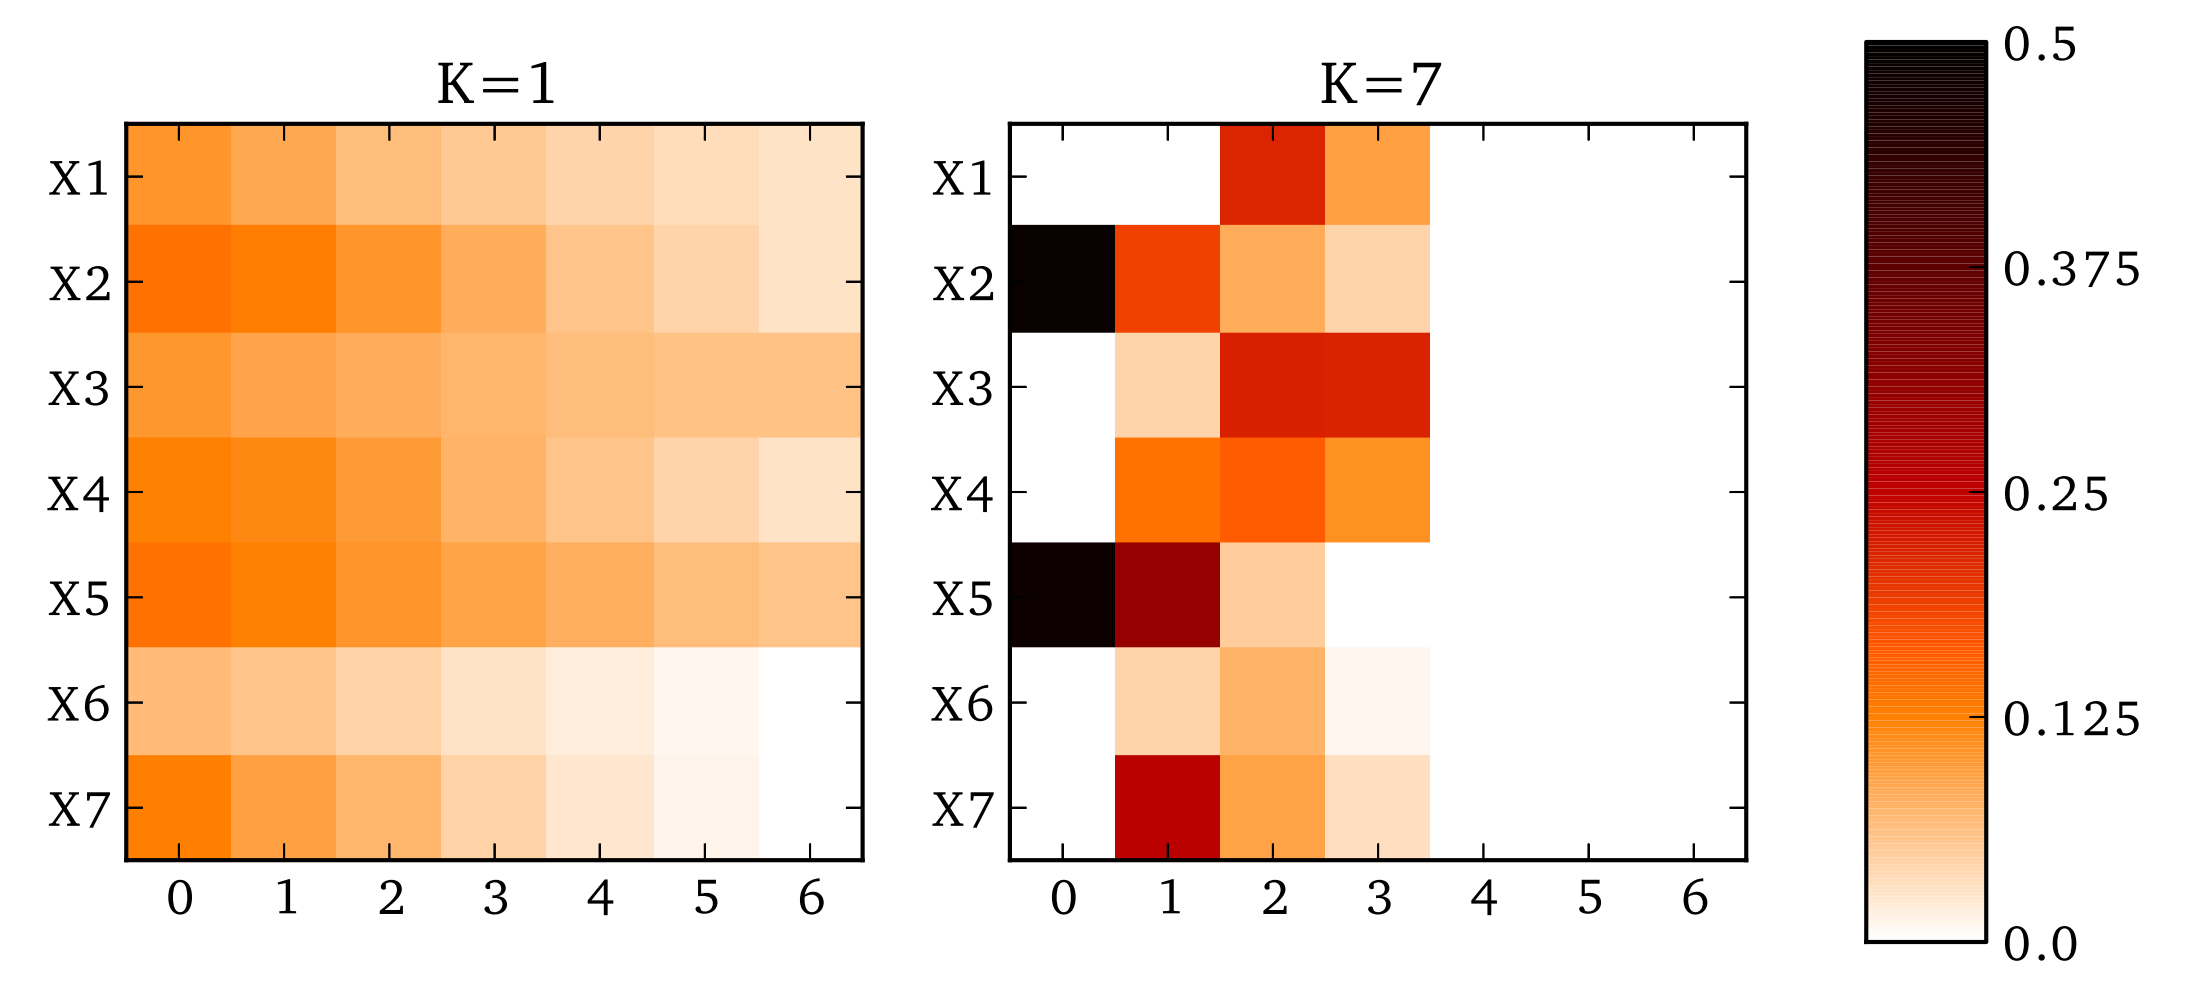
\includegraphics[width=0.45\textwidth]{images/mdi_randomized_pic.png}
\caption{\label{fig:mdi_rand_pic}\centering Важность признаков в зависимости от мощности множества, на котором она обуславливается. Значение в клетке $(i, j)$ --- $j$-ое слагаемое из первой суммы в \eqref{mdi_rand:1} для $X_i$. На картинке слева используется обычное дерево, справа --- случайный лес~\citep{mdi_randomized}}
\end{wrapfigure}

где $\mathcal{P}_{k}\left(V^{-m}\right)$ --- множество подмножеств мощности $k$, не включающих признак $m$.
Формула \eqref{mdi_rand:1} даёт нам полноценное представление о зависимости признака и целевой переменной. Здесь присутствует разложение как по мощности множества взаимодействия с другими признаками (сумма по $k$), так и по её степени (сумма по подмножествам). Оказывается, если ограничить глубину деревьев до $q \leq p$, важность будет равна первым $q$ слагаемым из первой суммы в \eqref{mdi_rand:1}. Разбиение наглядно визуализируется на Рис.~\ref{fig:mdi_rand_pic}. Можно заметить, что некоторые признаки становятся неважными в присутствии других. В случае случайного леса признаки $X_2, X_5$ находились вверху дерева. Это привело к <<скрытым эффектам>>: часть признаков вносят свой вклад только при обуславливании с $X_2, X_5$.

Это также было замечено в~\citep{bias_rf}, где авторы предложили использовать имплементированный ими метод построения \emph{условных деревьев} (conditional trees [ctree]). Для каждого узла выбор переменной $X_j$ для расщепления осуществляется исходя из значений $p$-критериев независимости условного выхода $Y | X_i, i=\overline{1, p}$, посчитанного на основе данных, дошедших до узла. Такой подход в отличии от gini importance более устойчив к технике сэмплирования с возвратом в случайном лесе. Еще одним решением может стать \emph{перестановочная важность} (permutation importance). О ней пойдёт речь в секции \ref{wrap}.

\subsection{Wrapper методы}\label{wrap}
Наиболее простым и эффективным методом является \emph{перестановочная важность}. Для её вычисления необходимо сравнить выход модели на двух выборках: исходной и перемешанной по интересующему признаку. Такой подход сохраняет маргинальное распределение $\mathbf{X}_i$ и прост в вычислении, однако при сильнокоррелированных признаках он склонен занижать значимость, в частности, в случае аддитивной регрессионной модели~\citep{group_rf_2}. Данный подход можно развить и на группу признаков, как это сделано в статье~\citep{group_rf}:
\begin{gather*}
    \phi_{J}=\mathbb{E}\left[\left(\mathbf{Y}-\mathbf{a}\left(\mathbf{X}_{(J)}\right)\right)^{2}\right]-\mathbb{E}\left[(\mathbf{Y}-\mathbf{a}(\mathbf{X}))^{2}\right] = \operatorname{R}(\mathbf{a}, \mathbf{X}_{(J)}) - \operatorname{R}(\mathbf{a}, \mathbf{X}),\\
    \hat{\phi_{J}}=\frac{1}{N_{T}} \sum_{T}\left[\hat{\operatorname{R}}\left(T, \operatorname{oob}(\mathbf{\hat{X}}_{(J)}, T)\right)-\hat{\operatorname{R}}\left(T, \operatorname{oob}(\mathbf{\hat{X}}, T)\right)\right].
\end{gather*}
где $\hat{~}$ обозначает эмпирический аналог, $\mathbf{X}_{(J)}$ --- случайный вектор, полученный заменой в $\mathbf{X}$ случайных признаков $\mathbf{X}_{J}$ на их независимую от $\mathbf{Y}$ и оставшихся признаков копию, \hspace{1em} $\operatorname{oob}(\mathbf{\hat{Z}}, T)$ --- те объекты $\mathbf{\hat{Z}}$, которые не попали в \emph{тренировочную выборку} дерева $T$. В случае аддитивной регрессионной модели $\phi_{J}$ пропорционален дисперсии ответов на соответствующем подмножестве признаков. С помощью \emph{графика частичной зависимости} (PDP) это можно наглядно увидеть.

\emph{Частичная зависимость} (partial dependence) может и сама быть инструментом для подсчета важности:
\begin{equation*}
    \operatorname{PD}^{\text{IndSet}}\left(x\right)=\mathbb{E}\left[\mathbf{a}(z) \mid z_{\text {IndSet }}=x_{\text {IndSet }}\right], \hspace{1.0em} \text{IndSet}	\subseteq  \operatorname{IndP}.
\end{equation*}
В pyBreakDown~\citep{breakDown} авторы хотят найти такие признаки, чтобы при их небольшом возмущении прогноз  модели существенно изменился. Это они добиваются следующим образом. Начальное множество IndSet $= \varnothing$/$\operatorname{IndP}$. На каждой итерации алгоритма в/из IndSet добавляется/удаляется один признак. В первом варианте он максимизирует $\left|\operatorname{PD}^{\text {IndSet }}\left(x\right)-\operatorname{PD}\left(x\right)\right|$ (\emph{step-up}), во втором минимизирует (\emph{step-down}). В итоге получается последовательность признаков с убывающей/увеличивающейся важностью, так как она определяется, как разность между соответствующими $\operatorname{PD}(x)$ на соседних IndSet.

Можно сделать предположение, что важность признака больше, если он сильнее взаимодействует с другими. Это можно формально выразить через показатель~\citep{h2_score}:
\begin{equation*}
    \operatorname{H_{j}^{2}}=\sum_{i=1}^{n}\left[\mathbf{a}\left(x^{(i)}\right)-\operatorname{PD}^{\{j\}}\left(x^{(i)}\right)-\operatorname{PD}^{\{-j\}}\left(x^{(i)}\right)\right]^{2} / \sum_{i=1}^{n} \mathbf{a}^{2}\left(x^{(i)}\right),
\end{equation*}
где $\operatorname{PD}^{\{-j\}}$ = $\operatorname{PD}^{\operatorname{IndSet}}$, $\operatorname{IndSet} = \operatorname{IndP} \setminus \{j\}$.
$\operatorname{H_{j}^{2}}$ положительная и равна 0 тогда и только тогда, когда признак не взаимодействует с другими. Однако, как показано в разделе \ref{art_imortance}, это не очень подходящее определение значимости.

Рассмотрим один из самых популярных методов построения важности. Пусть у нас есть некоторая характеристическая функция $v: 2^{\operatorname{IndP}} \rightarrow \mathbb{R} $ такая, что $v(\varnothing)=0$. Будем искать определение важности, удовлетворяющее следующим свойствам:
\begin{itemize}[noitemsep]
    \item \emph{сумма в конечный ответ} (efficiency): $\sum_{i \in \operatorname{IndP}} \phi_{i}(v)=v(\operatorname{IndP})$,
    \item \emph{аддитивность} (additivity): $\forall v, w: \phi(v+w)=\phi(v)+\phi(w)$, где $(v+w)(S)=v(S)+w(S)$ $\forall S  \subseteq \operatorname{IndP}$,
    \item \emph{симметрия} (symmetry): Если $v(S \cup\{i\})=v(S \cup\{j\})$ $\forall S$, где $S \subset \operatorname{IndP}$ и $i, j \notin S$, тогда $\phi_{i}(v)=\phi_{j}(v)$,
    \item \emph{корректность} (dummy): Если $v(S \cup\{i\})=v(S)$ $\forall S$, где $S \subset \operatorname{IndP}$ и $i \notin S$, тогда $\phi_{i}(v)=0$.
\end{itemize}
Оказывается аддитивность и симметричность вместе эквивалентна \emph{согласованности} \newline
(consistency)~\citep{deepshap}: Если $\forall v, w; \forall S:i \notin S$ выполнено $v(S \cup\{i\}) - v(S) \geq w(S \cup\{i\}) - w(S)$, тогда $\phi_{i}(v) \geq \phi_{i}(w)$. Существует единственная важность, удовлетворяющая данным требования. Это \emph{Shapley values}:
\begin{equation*}
    \operatorname{S h_{i}(v)}=\sum_{S \hspace{0.1em}\subseteq\hspace{0.1em} \operatorname{IndP} \backslash\{i\}} \frac{1}{p} \frac{1}{{p-1\choose |S|}} (v(S \cup\{i\})-v(S)), \quad i=\overline{1, p}.
\end{equation*}
В данном случае учитывается вклад $i$-ого признака во всевозможные подмножества других. В~\citep{shap_perm} рассматривается другой подход задать такие значения, помогающий избежать экспоненциальной сложности:
\begin{gather*}
    \phi_{i}=\frac{1}{p ! \cdot|\mathcal{X}|} \sum_{O \in \pi(p)} \sum_{y \in \mathcal{X}}\left[\mathbf{a}\left(\tau\left(x, y, \operatorname{Pre}^{i}(O) \cup\{i\}\right)\right)-\mathbf{a}\left(\tau\left(x, y, \operatorname{Pre}^{i}(O)\right)\right)\right],\\
    \tau(x, y, S)=\left(z_{1}, z_{2}, \ldots, z_{p}\right), \quad z_{i}=\left\{\begin{array}{ll}
    x_{i} & ; \quad i \in S \\
    y_{i} & ; \quad i \notin S
    \end{array}\right.
\end{gather*}
где $\pi(p)$ --- множество упорядоченных перестановок длины $p$, $\operatorname{Pre}^{i}(O)$ --- множество индексов, которые стоят перед $i$ в $O \in \pi(p)$. Авторы считают $65000 \cdot p$ итераций совместного сэмплирования перестановки и элемента выборки достаточным для аппроксимации с ошибкой 0.01 для 99\% переменных.

Рассмотрим некоторые нейросетевые определения значимости признаков. Метод DeepLift ~\citep{deep_lift} основан на разделении отрицательного и положительного вклада в целевую переменную. Таким образом возможно избежать некоторые проблемы, связанные с обнулением градиентов и отсутствием изменения ответов модели при перестановке входов. Пусть есть начальное значение $x_{m0}, y_0$. Положим $\Delta y = y - y_0, \Delta x_m = x_m - x_{m0}$, тогда:
$$
\phi_{m}=m_{\Delta x_{m} \Delta y} \Delta x_{m},
$$
где $m_{\Delta x_{m} \Delta y} = const$.
Выполняются свойства:
\begin{itemize}[noitemsep]
    \item \emph{Сумма в дельту} (summation to delta): $$
    \sum_{i=1}^{p} \phi_{i}=\Delta y.$$
    \item \emph{Цепное правило} (chain rule): $$m_{\Delta x_{i} \Delta y}=\sum_{j} m_{\Delta x_{i} \Delta z_{j}} m_{\Delta z_{j} \Delta y}.$$
\end{itemize}
Внутренние состояния пересчитываются через цепное правило и специальное определение мультипликаторов, которое учитывает появление <<знаковых $\Delta$>> в присутсвии или отсутствии $\Delta$ другого знака. Данный подход решил часть проблем, но некоторые всё же остаются. Например, трансформация коэффициентов при проходе через max\_pool слой.

Если посчитать для части модели коэффициенты $m_{\Delta x_{m} \Delta y}$, используя Shapley values, получим DeepShap~\citep{deepshap}.

Shapley values можно аппроксимировать с помощью линейной регрессии, если взять MSE лосс с определенным ядром. Тогда мы получим так называемый Kernel SHAP~\citep{deepshap}. Он сходится гораздо быстрее в отличии от простого сэмплирования Shapley values.

\begin{wrapfigure}{R}{0.35\textwidth}
\centering
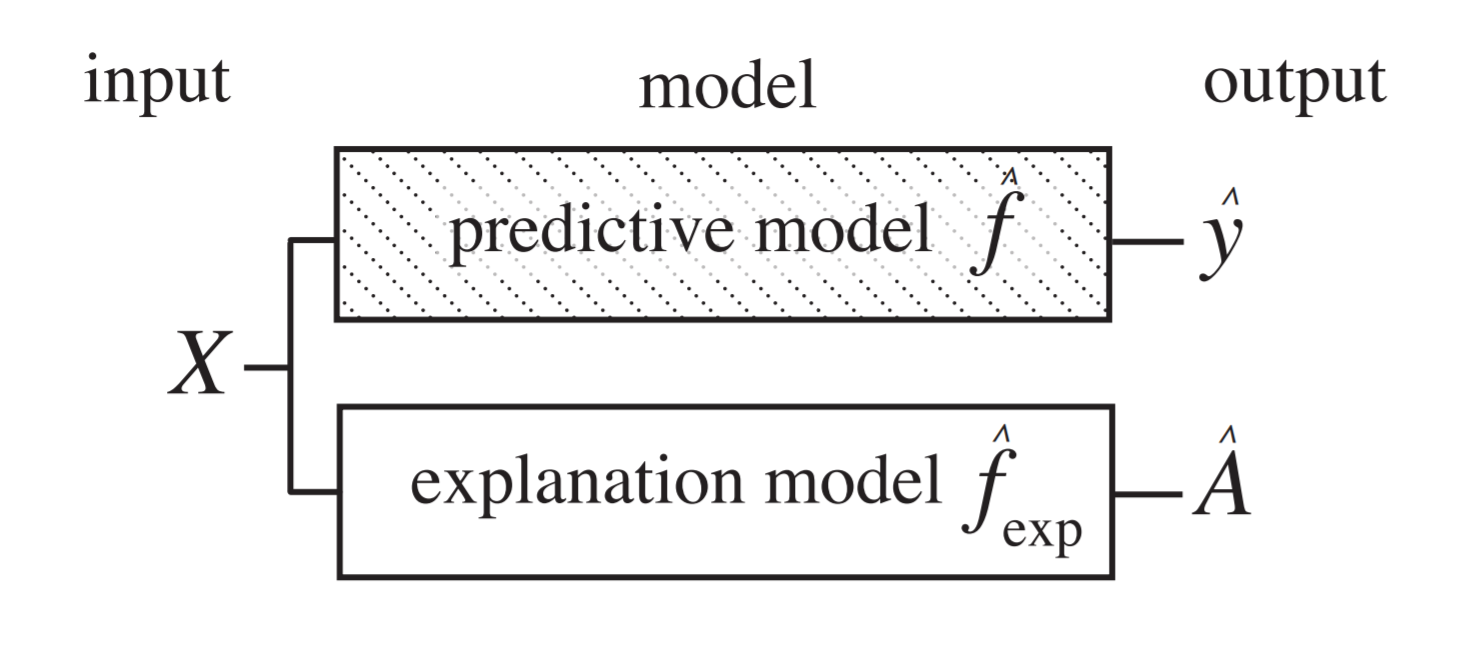
\includegraphics[width=0.35\textwidth]{images/exp_model.png}
\caption{\label{fig:exp_model}\centering Важность в CXPlain. Объясняющая модель $\hat{f}_{\exp }$ обучается выдавать важность признаков $\hat{A}$ для исходной модели $\hat{f}$~\citep{CXplain}}
\end{wrapfigure}
Другой подход связан с построением так называемой \emph{объясняющей модели} (explanation model). В CXplain~\citep{CXplain} используется Granger's определение причинности взаимосвязи между признаками и целевой переменной, в котором:
\begin{itemize}[noitemsep]
    \item все признаки релевантные,
    \item признак временно предшествует метке, то есть для того, чтобы получить метку, нужна информация о признаке.
\end{itemize}
Важность определяется как нормированная разница ошибок объясняемой модели на маскированных данных и исходных. У объясняющей модели:
\begin{itemize}[noitemsep]
    \item цель --- предсказать важность признаков,
    \item вход --- элемент из выборки,
    \item лосс --- расстояние Кульбака — Лейблера между истинным и предсказанным распределениями важности признаков.
\end{itemize}
Заметим, что данная модель нужна когда нет истинных меток объектов. Маскирование  $X_i$ подразумевает замену значений в $X_i$ на другие так, чтобы связь с оставшимися признаками пропала. Замену значений можно осуществить несколькими способами: усреднить значения признака, заполнить константой, перемешать. Для устойчивости авторы обучают ансамбль обучающих моделей на сэмплированных выборках. Итоговая важность --- медиана предсказаний ансамбля, а точность --- интерквартильный размах. В таком подходе точность оценки важности коррелирует с ошибкой ранжирования важности признаков. Даже  при небольшой мощности ансамбля хорошо оценивается точность. Сильной стороной данного метода является быстрота, что как мы помним, оказалась краеугольным камнем в Shapley values.

\subsection{Mix методы}
\begin{figure}[h]
\centering
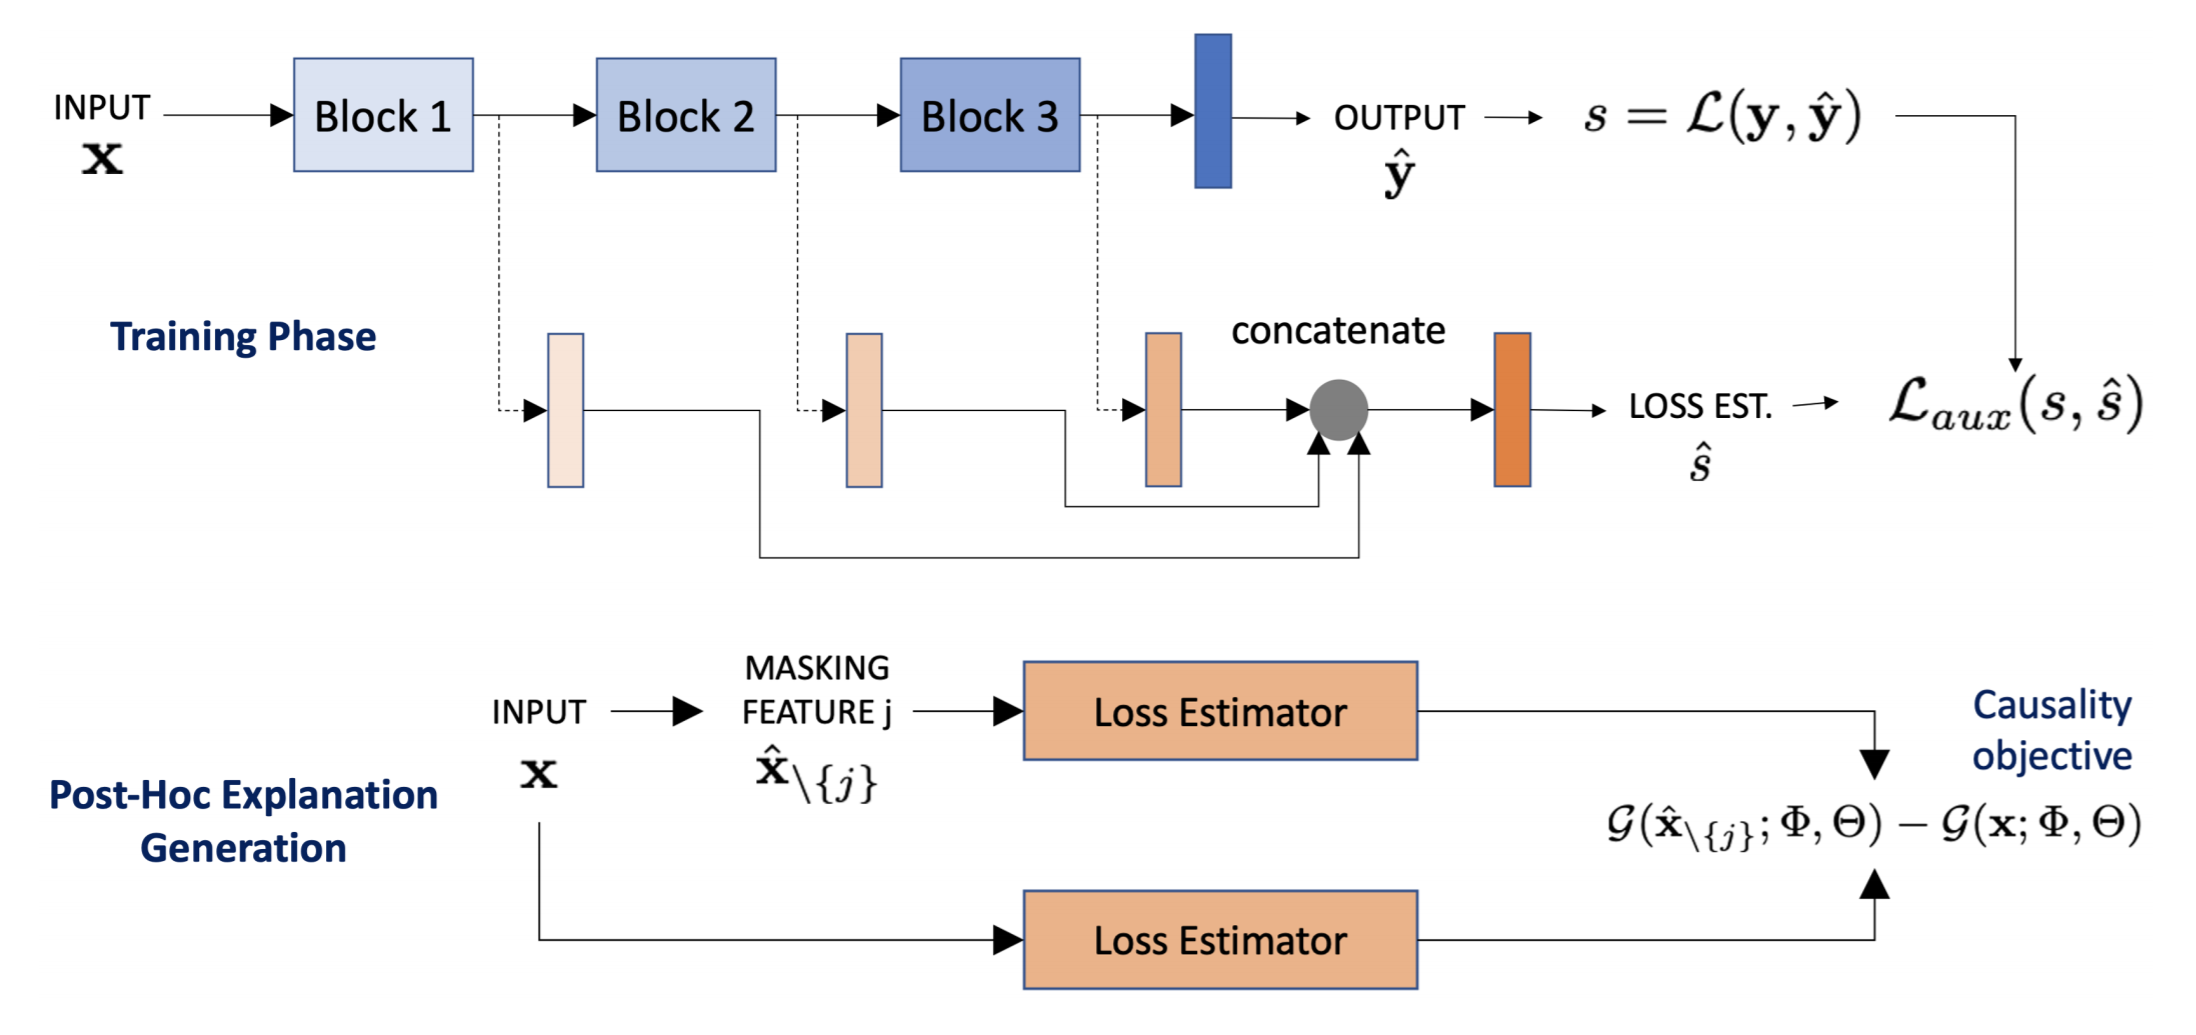
\includegraphics[width=150mm]{images/Profile.png}
\caption{\label{fig:profile}\centering Схема работы алгоритма получения важности в PRoFILE. Синим цветом отмечена исходная модель, а коричневым --- объясняющая~\citep{PRoFILE}}
\end{figure}
Использование не только выходов исходной модели, а также её внутреннего представления и знания о лоссе дают возможность построить <<хорошую>> объясняющую модель. 
В PRoFILE (см.~рис.~\ref{fig:profile}) у нее:
\begin{itemize}[noitemsep]
    \item цель --- научиться предсказывать лосс основной сети,
    \item вход --- латентные представления после некоторых слоёв основной сети, за каждым из которых следует линейный слой,
    \item лосс --- $\sum_{(i, j)} \max \left(0,-\mathbb{I}\left(s_{i}, s_{j}\right) \cdot\left(\hat{s}_{i}-\hat{s}_{j}\right)+\gamma\right) ,\\
    $ где $ \mathbb{I}\left(s_{i}, s_{j}\right)=\left\{
    \begin{array}{ll} 1 & \text {, если } s_{i}>s_{j} \hspace{6em} s_*=\mathcal{L}_{main net}(y_*, \mathbf{a}(x_*)),\\
    0 & \text {, иначе } \hspace{8.4em} \hat{s}_*=\mathcal{L}_{exp net}(s_*, \operatorname{exp\_model}(x_*)).
    \end{array}\right.
    $
\end{itemize}
Стоит заметить, что градиент от ошибки объясняющей модели влияет на слои в основной. Таким образом, мы тренируем модели совместно. В отличии от Shap, CXplain и Lime данный подход устойчив к <<помехам>> в данных: на датасетах  Cifar10-C, MNIST-USPS PRoFILE оказался лучше по показателю качества:
\begin{equation*}
    \Delta \text { log-odds }=\text { log-odds }\left(p_{\text {ref }}\right)-\text { log-odds }\left(p_{\text {masked }}\right),
\end{equation*}
где $\text { log-odds }(\mathrm{p})=\log \left(\frac{\mathrm{p}}{1-\mathrm{p}}\right)$, $\mathrm{p}_{\mathrm{ref}}$ --- вероятность, полученная на оригинальных данных, а $\mathrm{p}_{\text {masked }}$ --- на маскированных.

Рассмотрим другой подход. Допустим мы знаем заранее важность скольких признаков хотим найти, например, $s$ штук. Тогда логичным способом получения таких $\phi_{i}$ может стать обучение нейронной сети, которая выдает нам набор переменных, входящих в интересующее множество. В одном из методов ранжирования оценок важности признаков (FIR) (см.~рис.~\ref{fig:fir}) обучение происходит поочередно.
Оно сочетает в себе два этапа, где маски для признаков --- бинарные вектора (1 - берем признак, 0 - нет) длины $d$:

\begin{figure}[h]
\centering
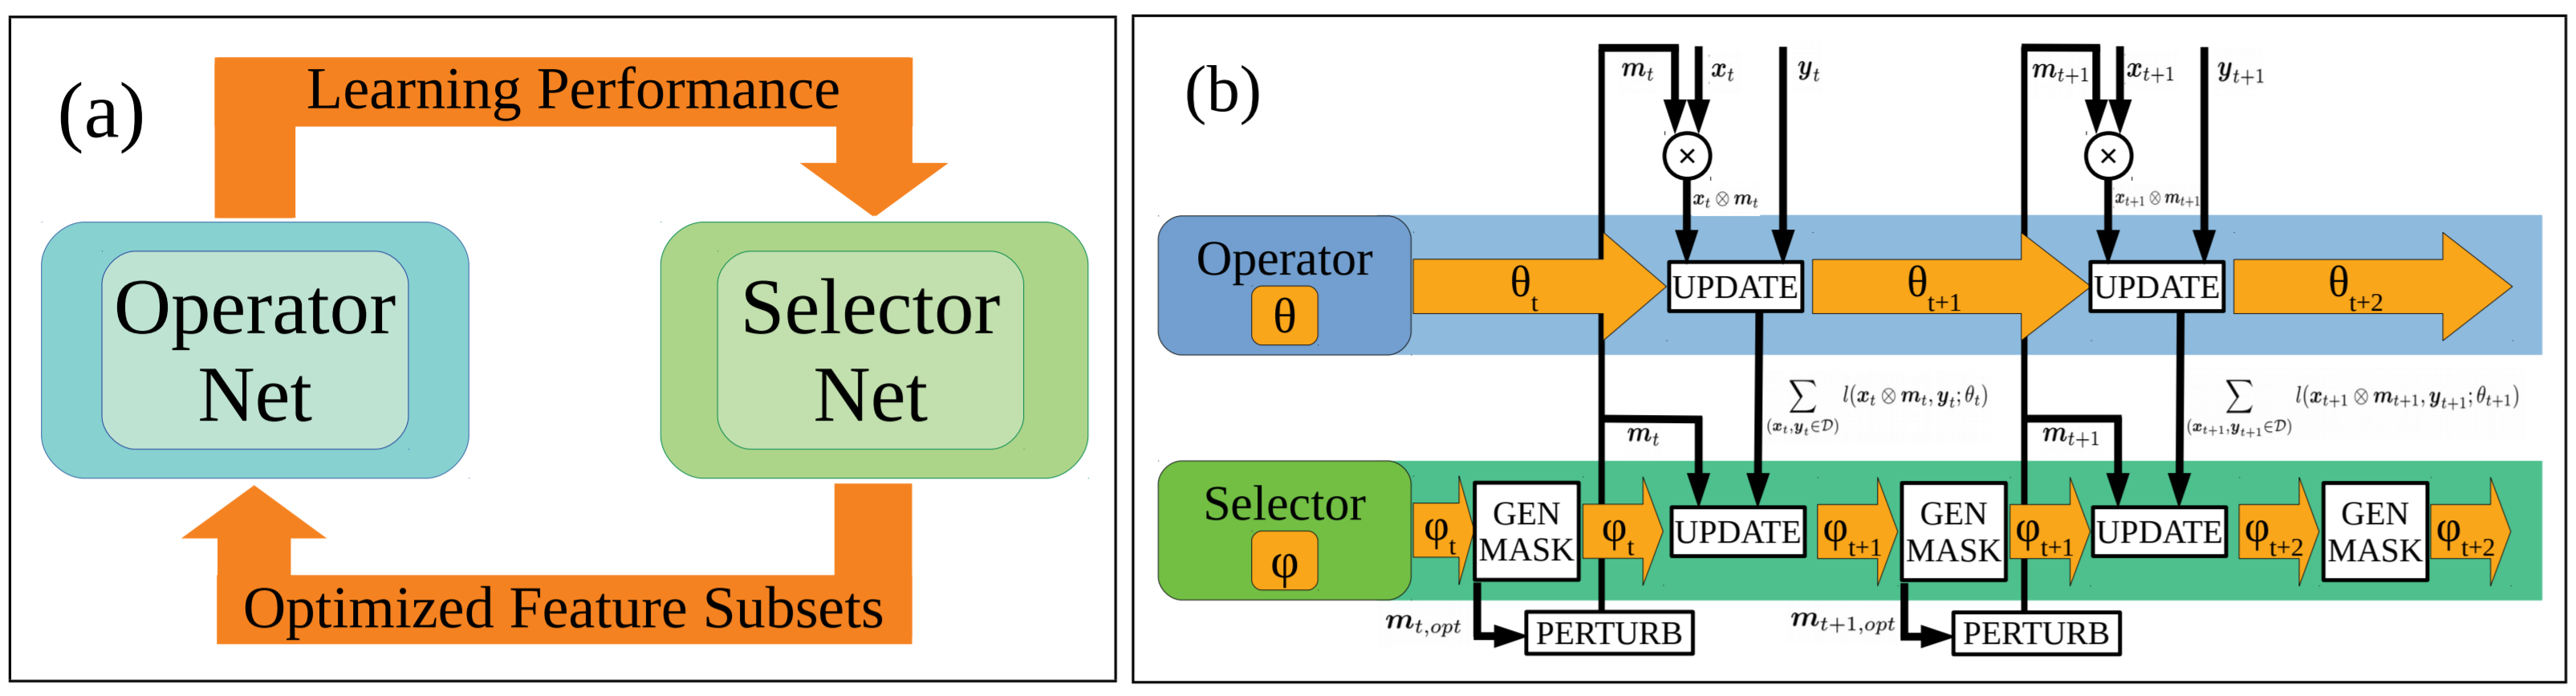
\includegraphics[width=150mm]{images/FIR.png}
\caption{\label{fig:fir}\centering Схема работы алгоритма получения важности в FIR~\citep{FIR}}
\end{figure}
\begin{enumerate}[noitemsep]
    \item operator net генерирует обучающую выборку для selector net: пары масок и соответствующий лосс на них
    \item selector net передаёт operator net'у следующие <<хорошие>> маски:
    \begin{enumerate}
        \item лучшая маска с предыдущей итерации,
        \item маска, получаемая результатом следующего алгоритма:
        \begin{enumerate}
            \item стартуем с маски $\boldsymbol{m}_{0}=\left(\frac{1}{2}, \cdots, \frac{1}{2}\right)$, выбираем топ $s$ компонент градиента selector net'а. Валидируем полученную <<оптимальную>> маску:
            \begin{enumerate}
                \item берем топ $s$ компонент градиента только теперь уже в точке, равной полученной маске. Таким образом получаем две маски: $\boldsymbol{m}_{\text {opt }}$ --- содержит $s$ единиц, $\overline{\boldsymbol{m}}_{\text {opt }}$ --- содержит $d-s$ единиц.
                \item заменяем компоненту маски $\boldsymbol{m}_{\text {opt }}$ с отрицательным градиентом на компоненту с наибольшим градиентов в маске $\overline{\boldsymbol{m}}_{\text {opt }}$
                \item проверяем условие $\operatorname{selector\_net}\left(\boldsymbol{m}_{o p t}\right) \leq \operatorname{selector\_net}\left(\boldsymbol{m}_{o p t}^{\prime}\right)$, где $\boldsymbol{m}_{\text {opt }}^{\prime}$ получена заменой компоненты маски $\boldsymbol{m}_{o p t}$ с наименьшим градиентом на компоненту маски $\overline{\boldsymbol{m}}_{\text {opt }}$ с наибольшим. Если это условие не выполнено повторяем A.-B.
            \end{enumerate}
        \end{enumerate}
        \item полученная $\boldsymbol{m}_{\text {opt }}$ на самом деле может быть неоптимальной, поэтому добавляем небольшую случайность: случайно выберем $s_{rand} < s$ компонент в $\boldsymbol{m}_{\text {opt }}/\overline{\boldsymbol{m}}_{\text {opt }}$, инвертируем их и поменяем значения местами с другой маской. Сделаем так несколько раз. 
    \end{enumerate}
\end{enumerate}
В итоге у operator net:
\begin{itemize}[noitemsep]
    \item цель --- обучение с учителем конкретной задачи,
    \item вход --- $x$ и маска признаков,
    \item лосс --- соответствующий задаче.
\end{itemize}
А у selector net:
\begin{itemize}[noitemsep]
    \item цель --- предсказать loss operator net,
    \item вход --- маска признаков,
    \item лосс --- MSE с лоссом, переданным от operator net.
\end{itemize}
Важность признака --- соответствующая компонента градиента лосса selector net'а в точке оптимального набора признаков. Процесс построения оптимального набора очень долгий, но как показали результаты экспериментов, точность среди DFS, RF, RFE оказалась лучшая, как и качество выбранных признаков исходя из задачи. Однако время работы несравнимо больше: x$440$ дольше RF и x2 дольше Lime.

\newpage
\section{Эксперименты}
Во всех экспериментах участвуют следующие модели:
\begin{itemize}[noitemsep]
    \item \textbf{бустинг (LightGBM)} со стандартными параметрами,
    \item \textbf{метод опорных векторов (SVM)} с линейным ядром,
    \item \textbf{полносвязная нейронная сеть (MLP)} с параметрами:
        \begin{itemize}[noitemsep]
            \item 2 слоя,
            \item 64 нейронов на слой,
            \item dropout = 0.2 (с такой вероятностью выход нейрона случайно зануляется),
            \item batch\_size = 8,
            \item num\_epoch = 100,
            \item early\_stopping\_patience = 15.
        \end{itemize}
\end{itemize}
В качестве методов для оценки важности признаков выступают:
\begin{itemize}[noitemsep]
    \item \textbf{rfpimp (permutation)} --- перестановочная важность c f1 показателем качества,
    \item \textbf{eli5 (gain)} --- среднее увеличение количества информации для gini importance,
    \item \textbf{pyBreakDown (up)} --- описано в разделе \ref{wrap},
    \item \textbf{shap (Tree/Kernel)} --- для бустинга использовался вариант Tree, так как он позволяет посчитать истинные Shapley values. Однако сложность вычисления все равно достаточно большая для используемых данных, поэтому сэмплировалось приблизительно 100--200 объектов из выборки для подсчета важности $X_i$. Если мы работаем с SVM, то используется Kernel версия. Как отмечено раннее, она также приближает Shapley values, однако скорость сходимости и точность гораздо меньше по сравнению с Tree версией,
    \item \textbf{lime} --- метод взят из открытого источника~\citep{lime_git}, разработанного авторами данного метода~\citep{lime},
    \item \textbf{CXplain [exp\_m (p, mlp),  exp\_m (p, lgbm)]} --- CXplain c перемешивающим маскированием и MLP#/LightGBM в качестве объясняющей модели. Версия авторов метода в открытом доступе показала неинформативные результаты (все признаки одинаково важны). Поэтому была разработана аналогичная версия, где использовалась MSE/NLL ошибка в задаче регрессии/классификации,
    \item \textbf{permutation (nll)} --- перестановочная важность c nll ошибкой.
    Эта оценка важности является целевой переменой для объясняющей модели в CXplain (nll). 
\end{itemize}
Для таких методов, как pyBreakDown, shap, lime, CXplain важность $X_i$ получалась усреднением важности $X_i$ для всех объектов из \emph{валидационной выборки}. Код всех экспериментов можно найти по \href{https://github.com/MikhailKuz/3_course_diary/tree/master/experiments}{ссылке} на github репозиторий.


\subsection{Коррелированные признаки}\label{corr_expir}
\subsubsection{Данные}
Рассмотрим задачу классификации. Признаки состоят из пяти групп (gr$_1$, ..., gr$_5$) и одного шумового (rand). Каждая группа состоит из трёх признаков: gr$_{ij}$, j = 1, 2, 3. Группы независимы от друг друга и сэмплированы из нормального распределения $\mathcal{N}_{3}\left(0, C_{i}\right)$, где 
\begin{equation*}
    C_{i}=\left(\begin{array}{ccc}
1 & \rho_{i} & \rho_{i} \\
\rho_{i} & 1 & \rho_{i} \\
\rho_{i} & \rho_{i} & 1
\end{array}\right)
, \hspace{1em} \rho_{i} = \frac{i}{6}.
\end{equation*}
Шум был взят из распределения $\mathcal{N}_{3}\left(0, 1\right)$. Пусть $\boldsymbol{\xi}_i$ имеет биномиальное распределение \emph{Bi}$(1, 0.5)$. 
\newpage
Тогда целевая переменная $Y$ равна
\begin{gather*}
    \mathbb{I}[Z \geq \operatorname{median}(Z)], \hspace{1em}\text{где} \\
    Z = \operatorname{sigmoid}(\xi_1 \operatorname{gr}_{11} + ... + \xi_5 \operatorname{gr}_{51}).
\end{gather*}
В данной задаче признаки $\operatorname{gr}_{11}, ..., \operatorname{gr}_{51}$ одинаково важны для предсказания $Y$. Количество сэмплированных объектов равно 5000.

\subsubsection{Важность}\label{art_imortance}
Посчитаем $H_2$ score для наших данных.
\begin{figure}[h]
\centering
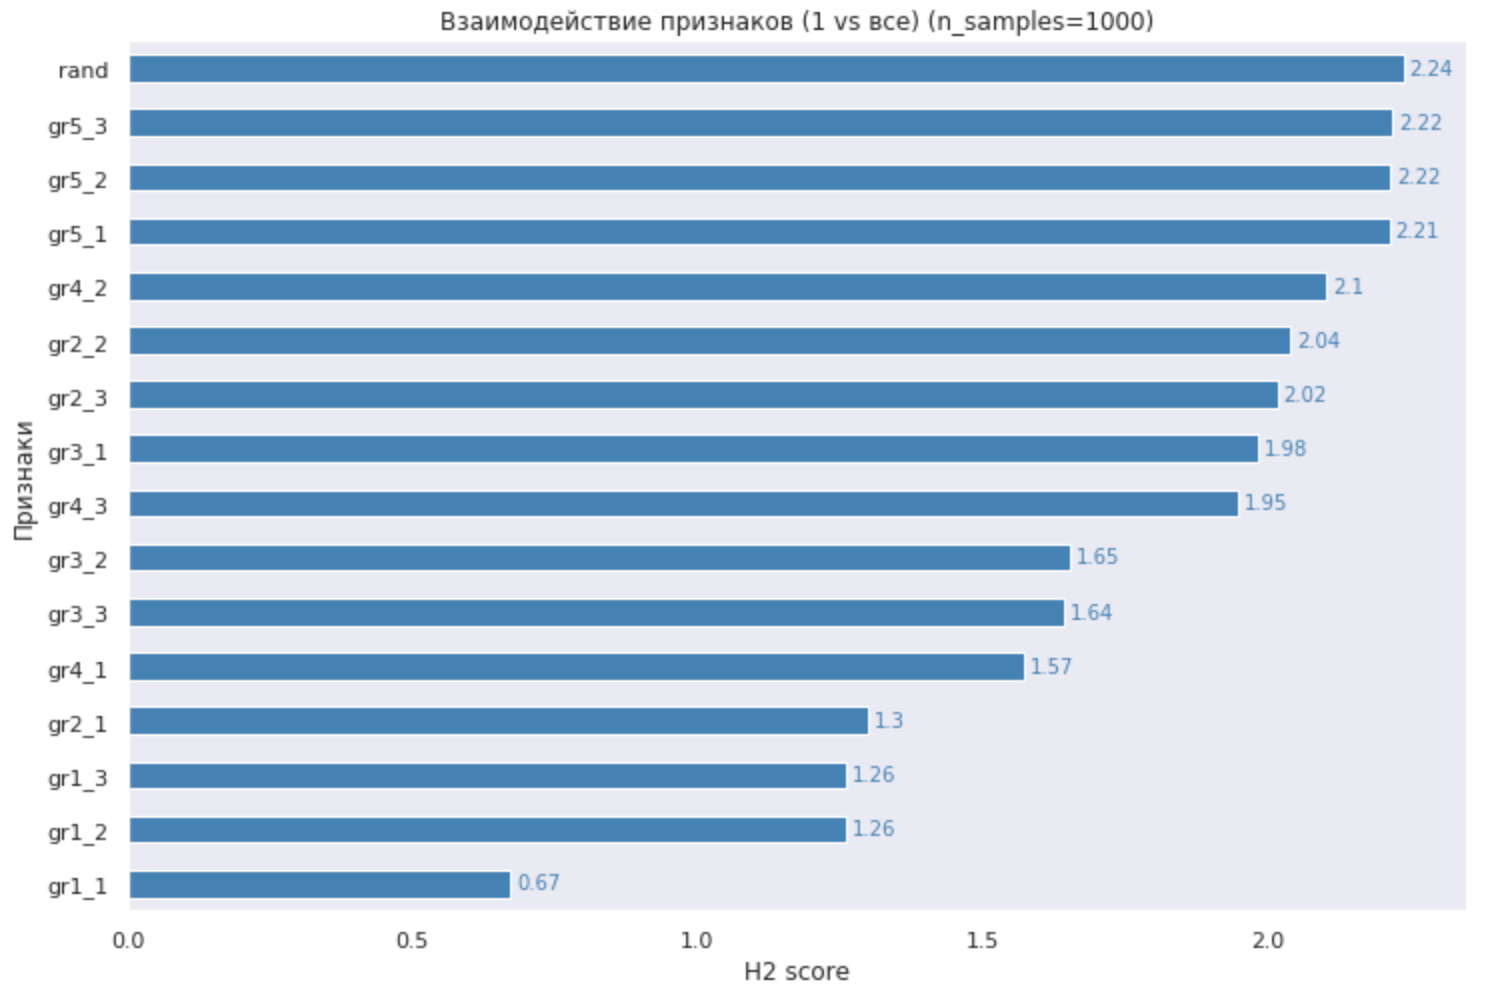
\includegraphics[width=150mm]{images/h2_art.png}
\end{figure}

Видно, что случайный признак оказался на первом месте. Чем больше групповые корреляции, тем больше взаимодействия получают признаки. 

\begin{figure}[h]
\centering
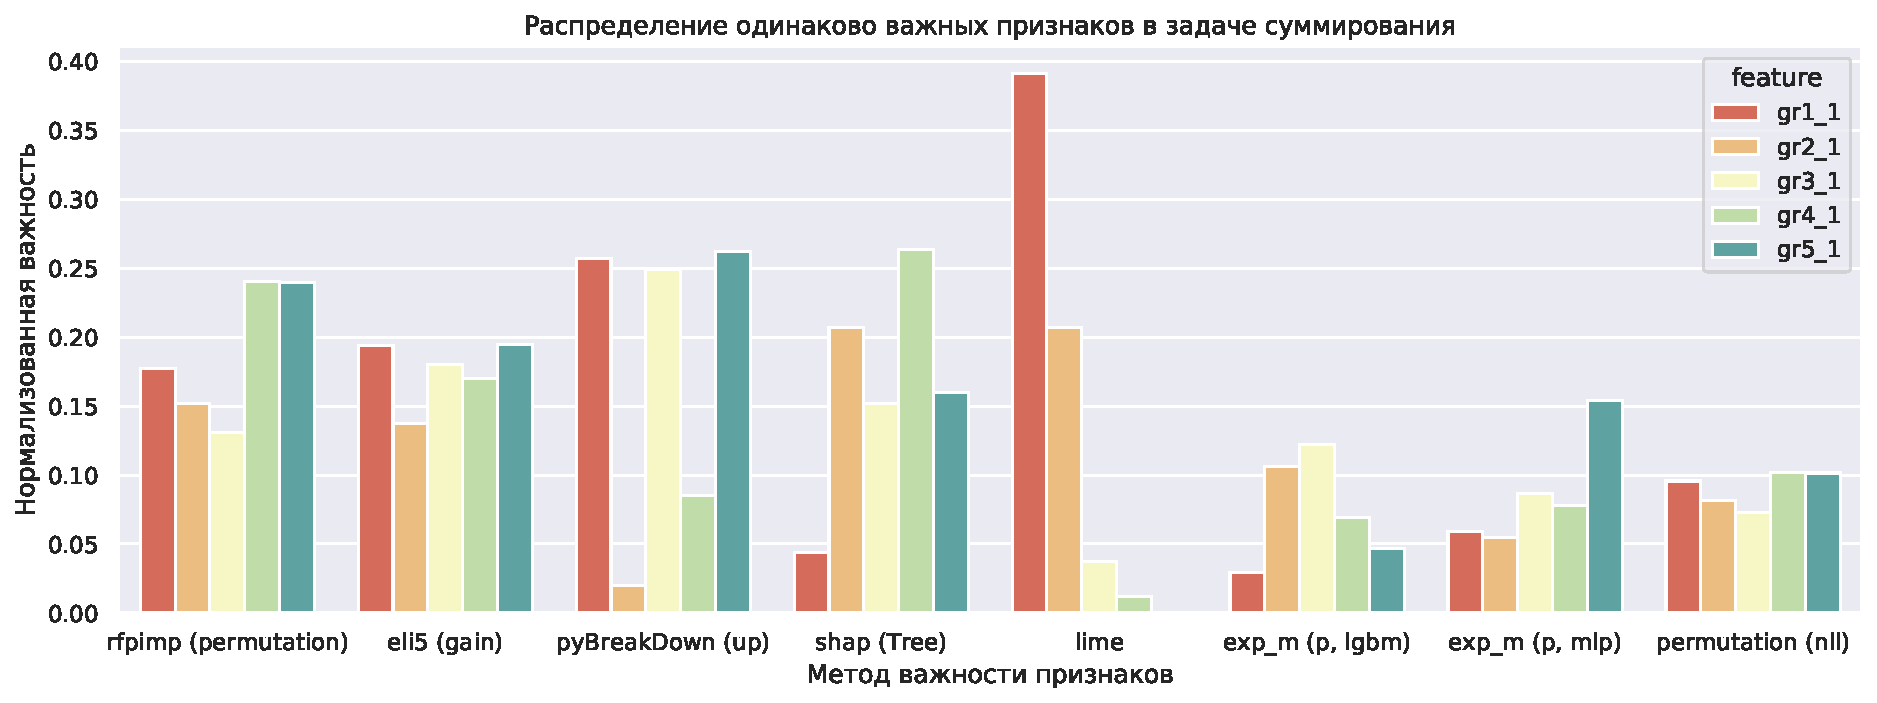
\includegraphics[width=\textwidth]{images/TargetSum_impFeatures.pdf}
\end{figure}
Наиболее равномерно распределены перестановочная, gain, Shapley, CXplain важности. Lime оставляет 2 наиболее важных признака, исходя из их независимости. Рассмотрим оценки важности признаков подробнее.
\newpage
\begin{figure}[h]
        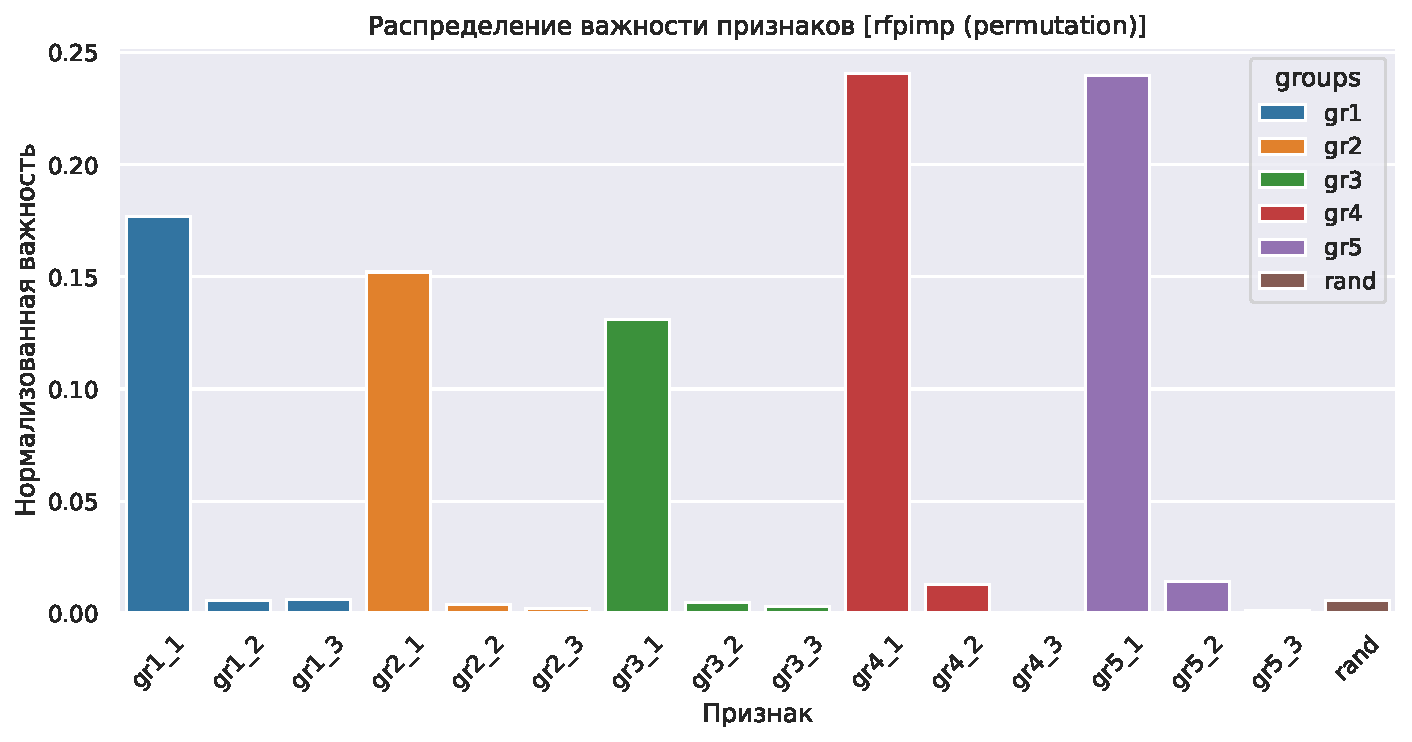
\includegraphics[width=0.5\textwidth]{images/TargetSum_allFeatures_rfpimp (permutation).pdf}
        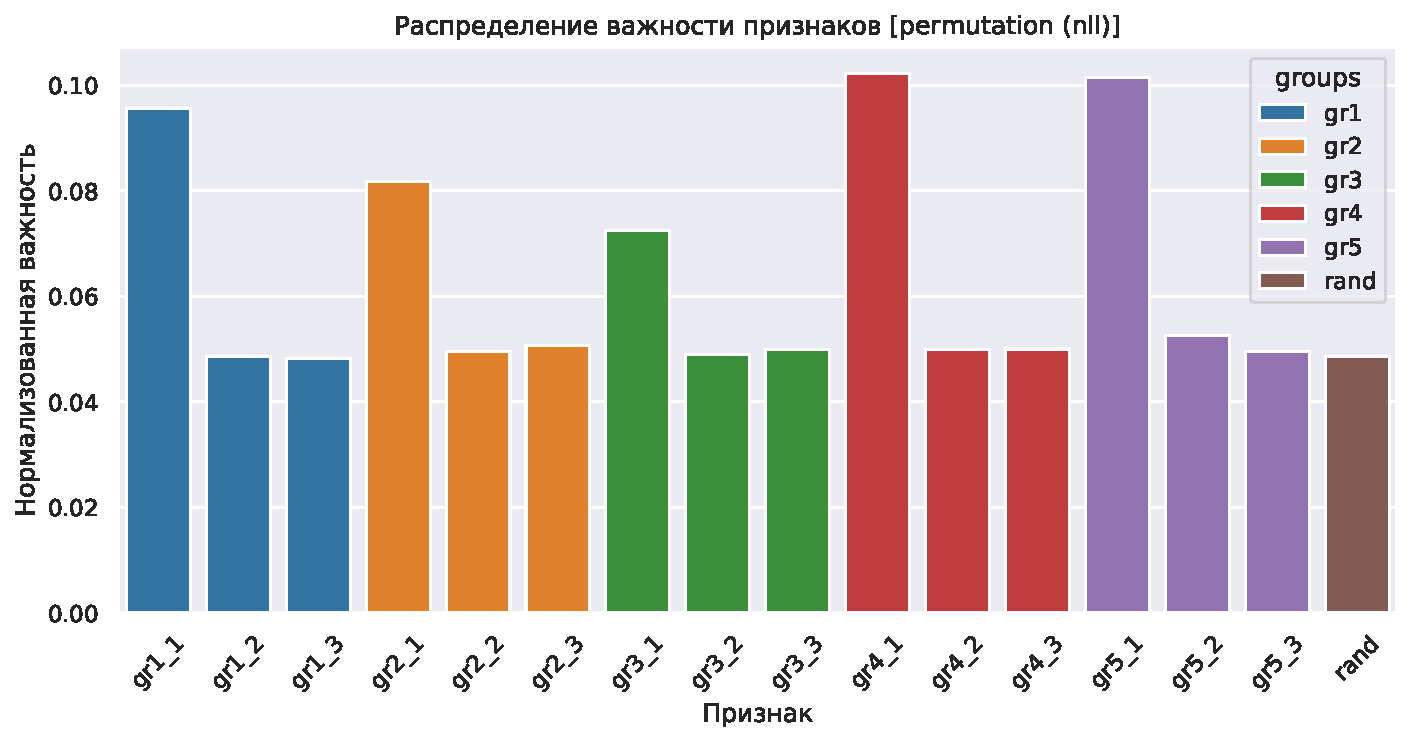
\includegraphics[width=0.5\textwidth]{images/TargetSum_allFeatures_permutation (nll).pdf}
        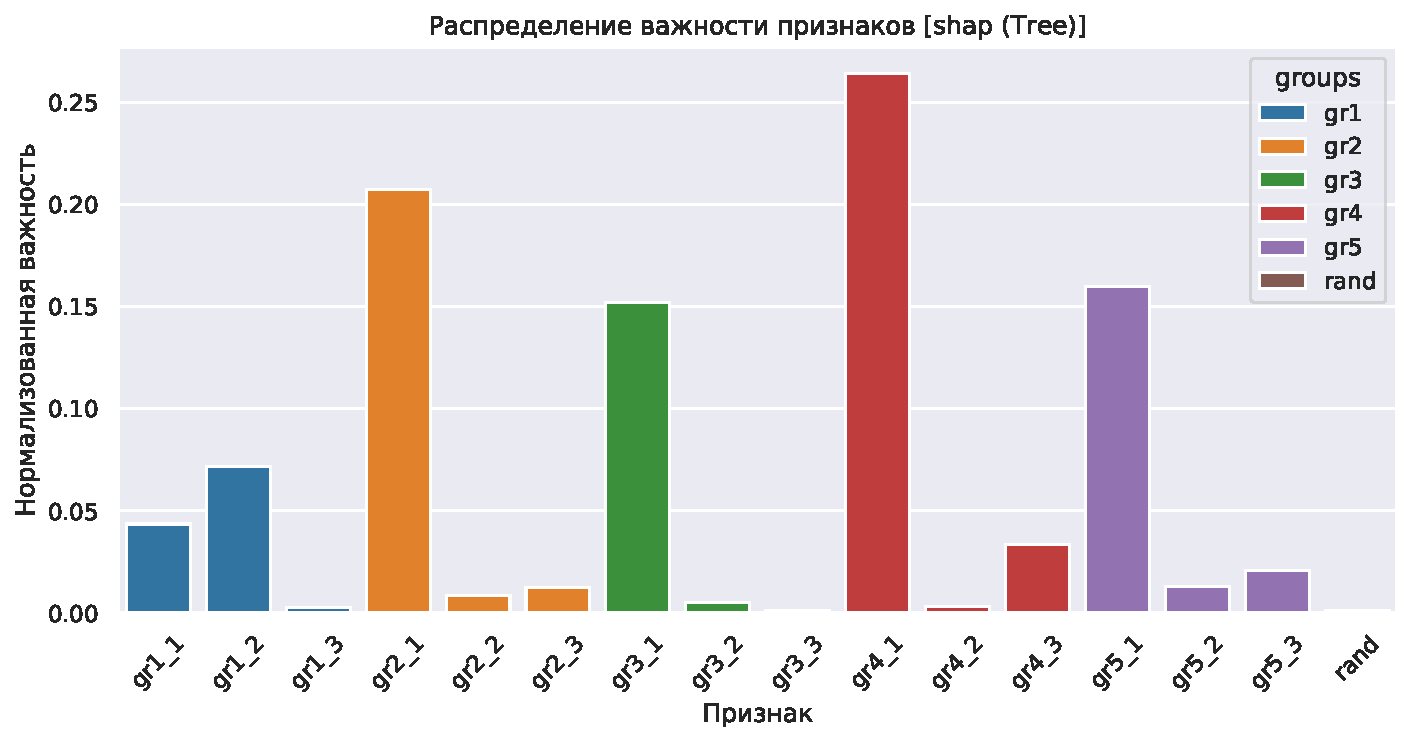
\includegraphics[width=0.5\textwidth]{images/TargetSum_allFeatures_shap (Tree).pdf}
        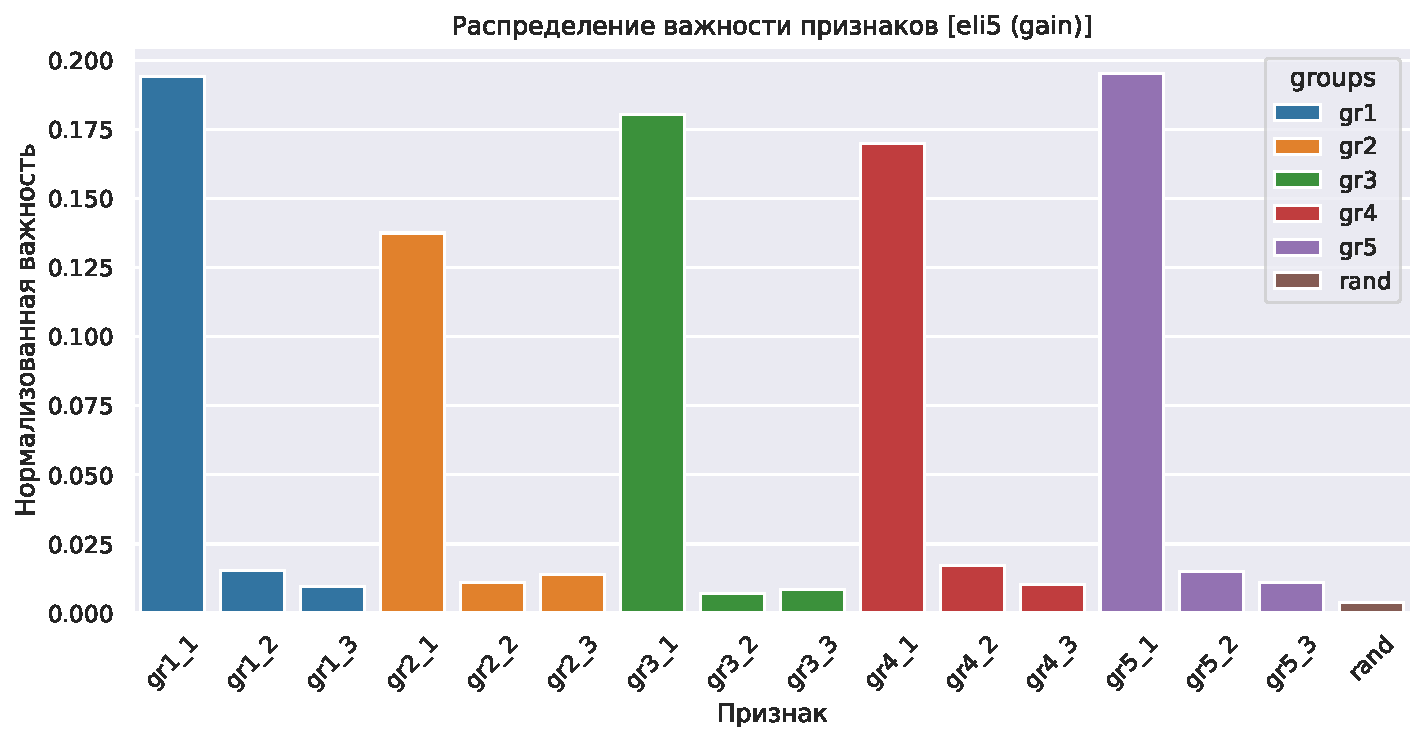
\includegraphics[width=0.5\textwidth]{images/TargetSum_allFeatures_eli5 (gain).pdf}
        \hfill
        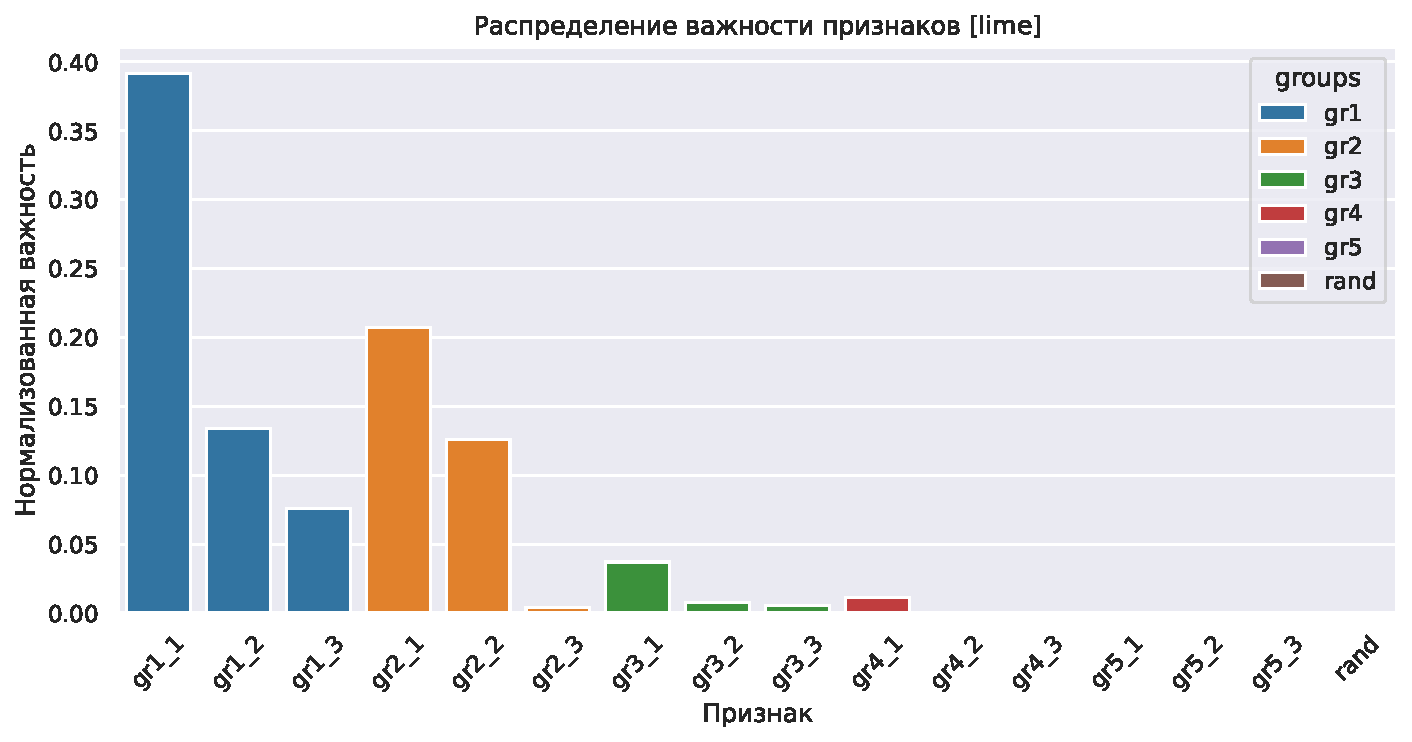
\includegraphics[width=0.5\textwidth]{images/TargetSum_allFeatures_lime.pdf}
        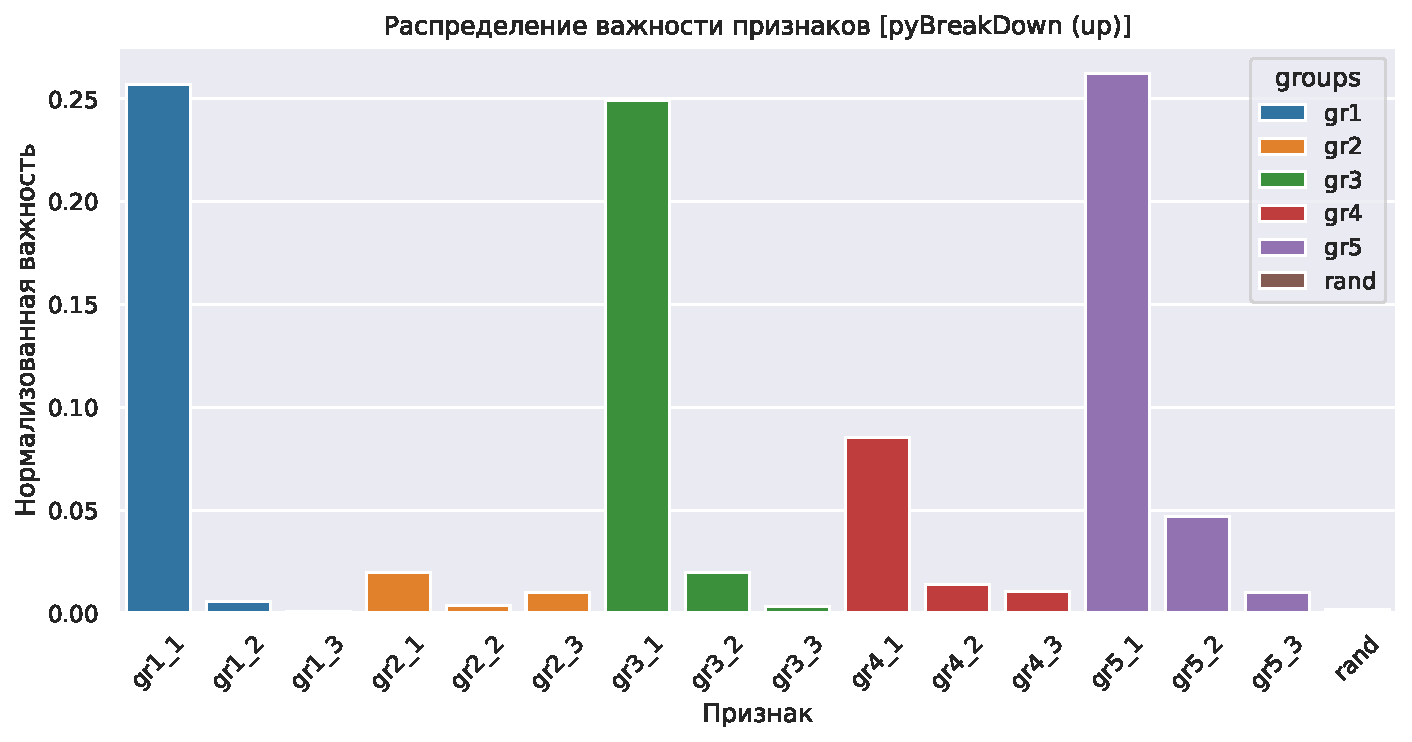
\includegraphics[width=0.5\textwidth]{images/TargetSum_allFeatures_pyBreakDown (up).pdf}
        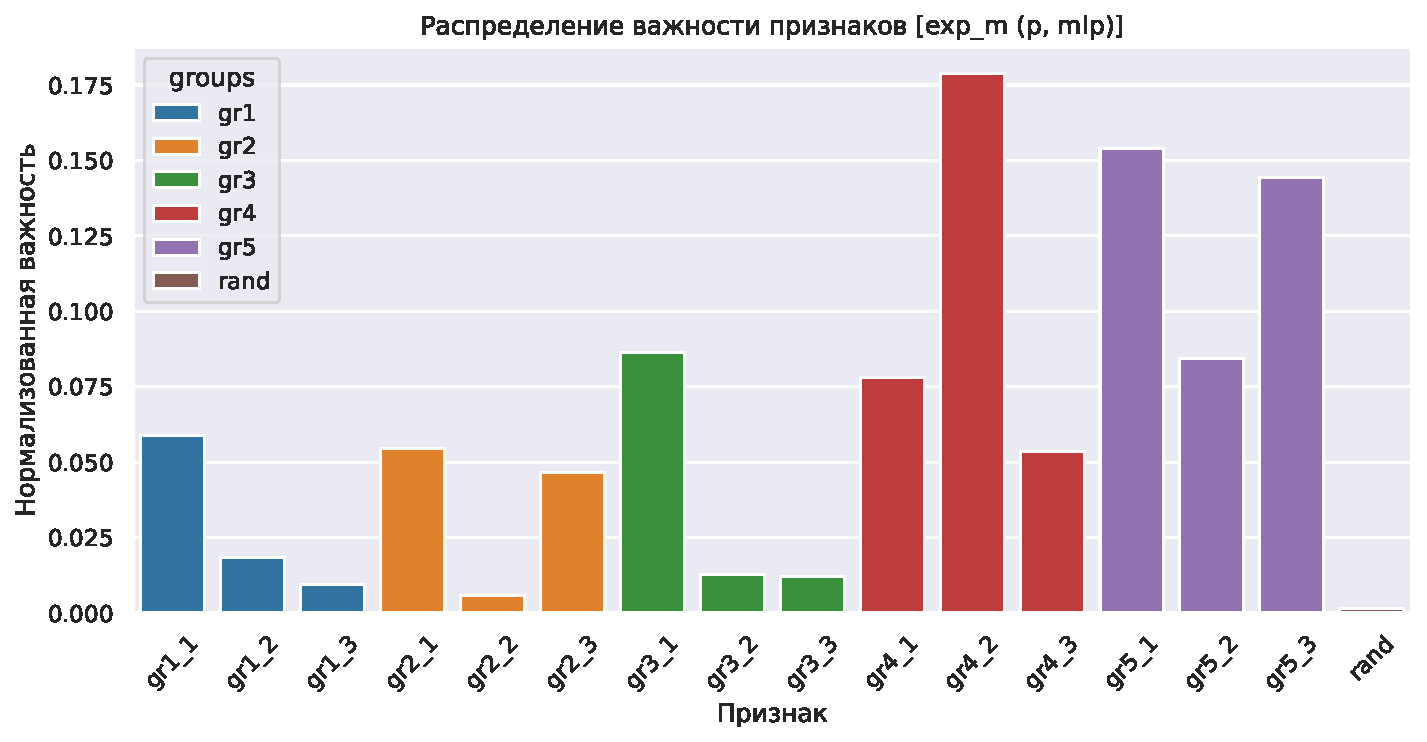
\includegraphics[width=0.5\textwidth]{images/TargetSum_allFeatures_exp_m (p, mlp).pdf}
        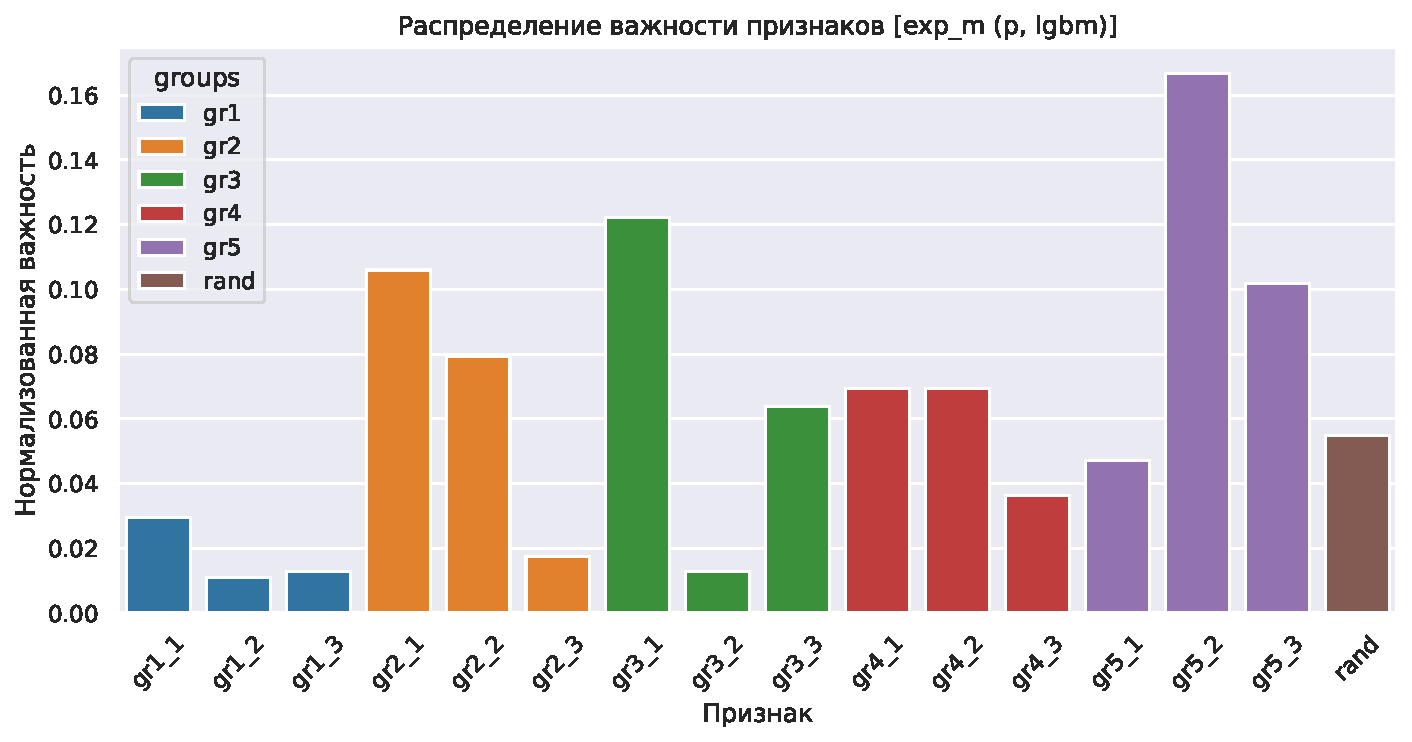
\includegraphics[width=0.5\textwidth]{images/TargetSum_allFeatures_exp_m (p, lgbm).pdf}
\end{figure}

Выбор оценочной функции для перестановочной функции важен. В данном случае f1 качество оказалась более подходящим. Shap устойчив к средним и большим корреляциям, но не к малым ($\operatorname{gr}_{12}$ самый важный в группе $\operatorname{gr}_{1}$, а не $\operatorname{gr}_{11}$). Стоит заметить практически нулевую важность случайного признака. Eli5 выдает одинаковую важность для групп с разной корреляцией, что говорит об его устойчивости к ней. Lime в силу своего построения отдает предпочтение малому количеству признаков, причем с характерным экспоненциальным убыванием важности. PyBreakDown склонен выделять с большой уверенностью небольшое количество важных признаков. Если выделить в каждой группе $\operatorname{gr}_i$ самый важный признак, то exp\_m (p, lgbm) и exp\_m (p, mlp) похожи. Однако есть несколько отличий. В exp\_m (p, mlp) чем больше групповая корреляция, тем больше суммарной важности в группе. Кроме того, для Lgbm важности признаков кажутся более хаотичными, что может свидетельствовать о переобучении. Относительно большая важность случайного признака также это подтверждает.


\newpage
\subsubsection{Удаление признаков}
Рассмотрим задачу рекурсивного удаления признаков (RFE). На каждой итерации удаляется наименее важный признак и замеряется качество на \emph{тестовой выборке}.
\begin{figure}[h]
\centering
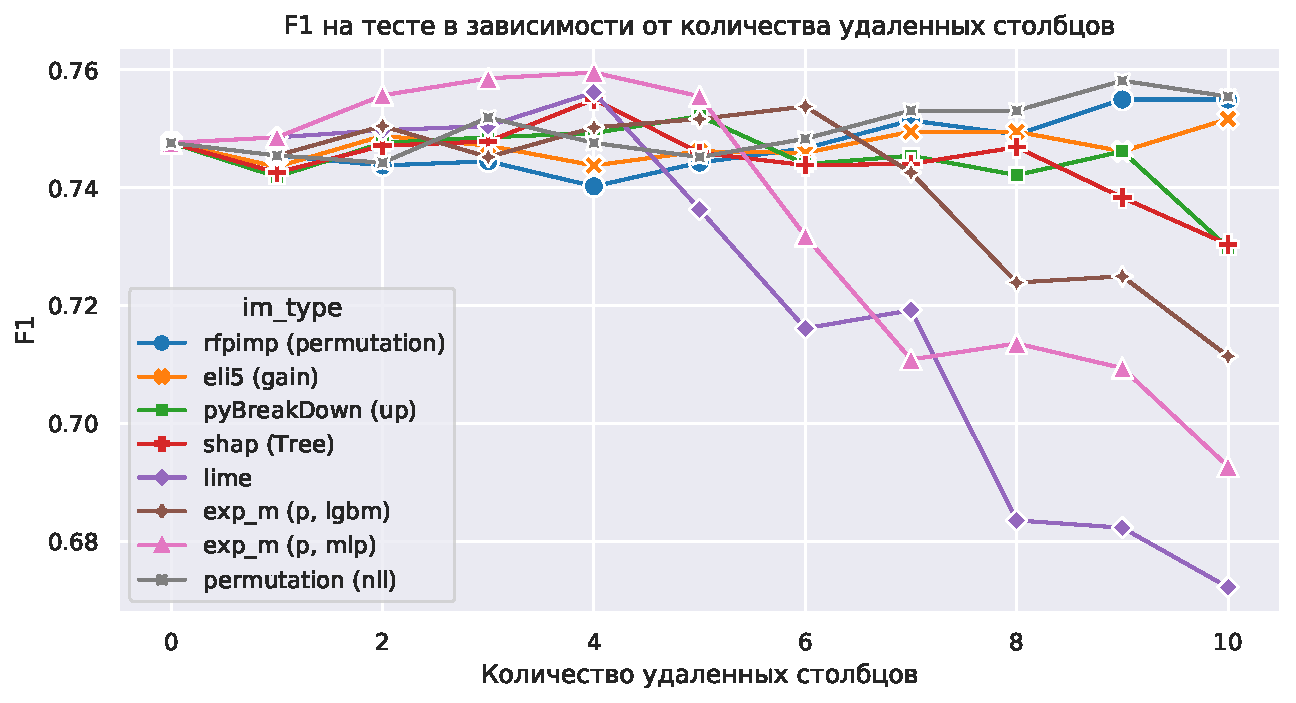
\includegraphics[width=0.8\textwidth]{images/RFE_f1.pdf}
\caption{\centering Один запуск эксперимента RFE. Конечное количество признаков $= 30\%$ от исходного. Для вычисления shap сэмплировались 200 объектов из выборки.}
\end{figure}

Перестановочная и gain важность лучше всего отбирают признаки <<на будущее>>. Для перестановочной важности ошибка nll (серая линия) оказалась все время не ниже ошибки f1 (синяя линия). Исходя из распределения оценок важности признаков для nll можно сделать вывод, что коррелированные переменные служат хорошей заменой друг другу. Дерево действительно инвариантно к сдвигу или масштабированию признака. 

Lime не учитывает зависимости второго и более порядков. Это может стать причиной выбрасывания относительно <<хороших>> признаков на ранних стадиях.

В идеальном варианте exp\_m оценки важностей должны совпадать с permutation (nll). Этого не происходит по двум вариантам: объясняющая модель слишком простая или мало данных. Учитывая, что обучение объясняющей модели происходило на валидационной выборке второй вариант вероятнее. 


\label{added_art}

\newpage
\subsubsection{Сэмплирование признаков}
Посмотрим, как важность хороша с точки зрения дальнейшего обучения м одели. Для каждого метода мы взяли нормализованный модуль важности и просэмплировали 1000 раз определенное количество признаков (30\%, 50\%, 70\% от исходного количества). После чего замерили качество (f1-качество) на \emph{тестовой выборке}.
\begin{figure}[h]
\centering
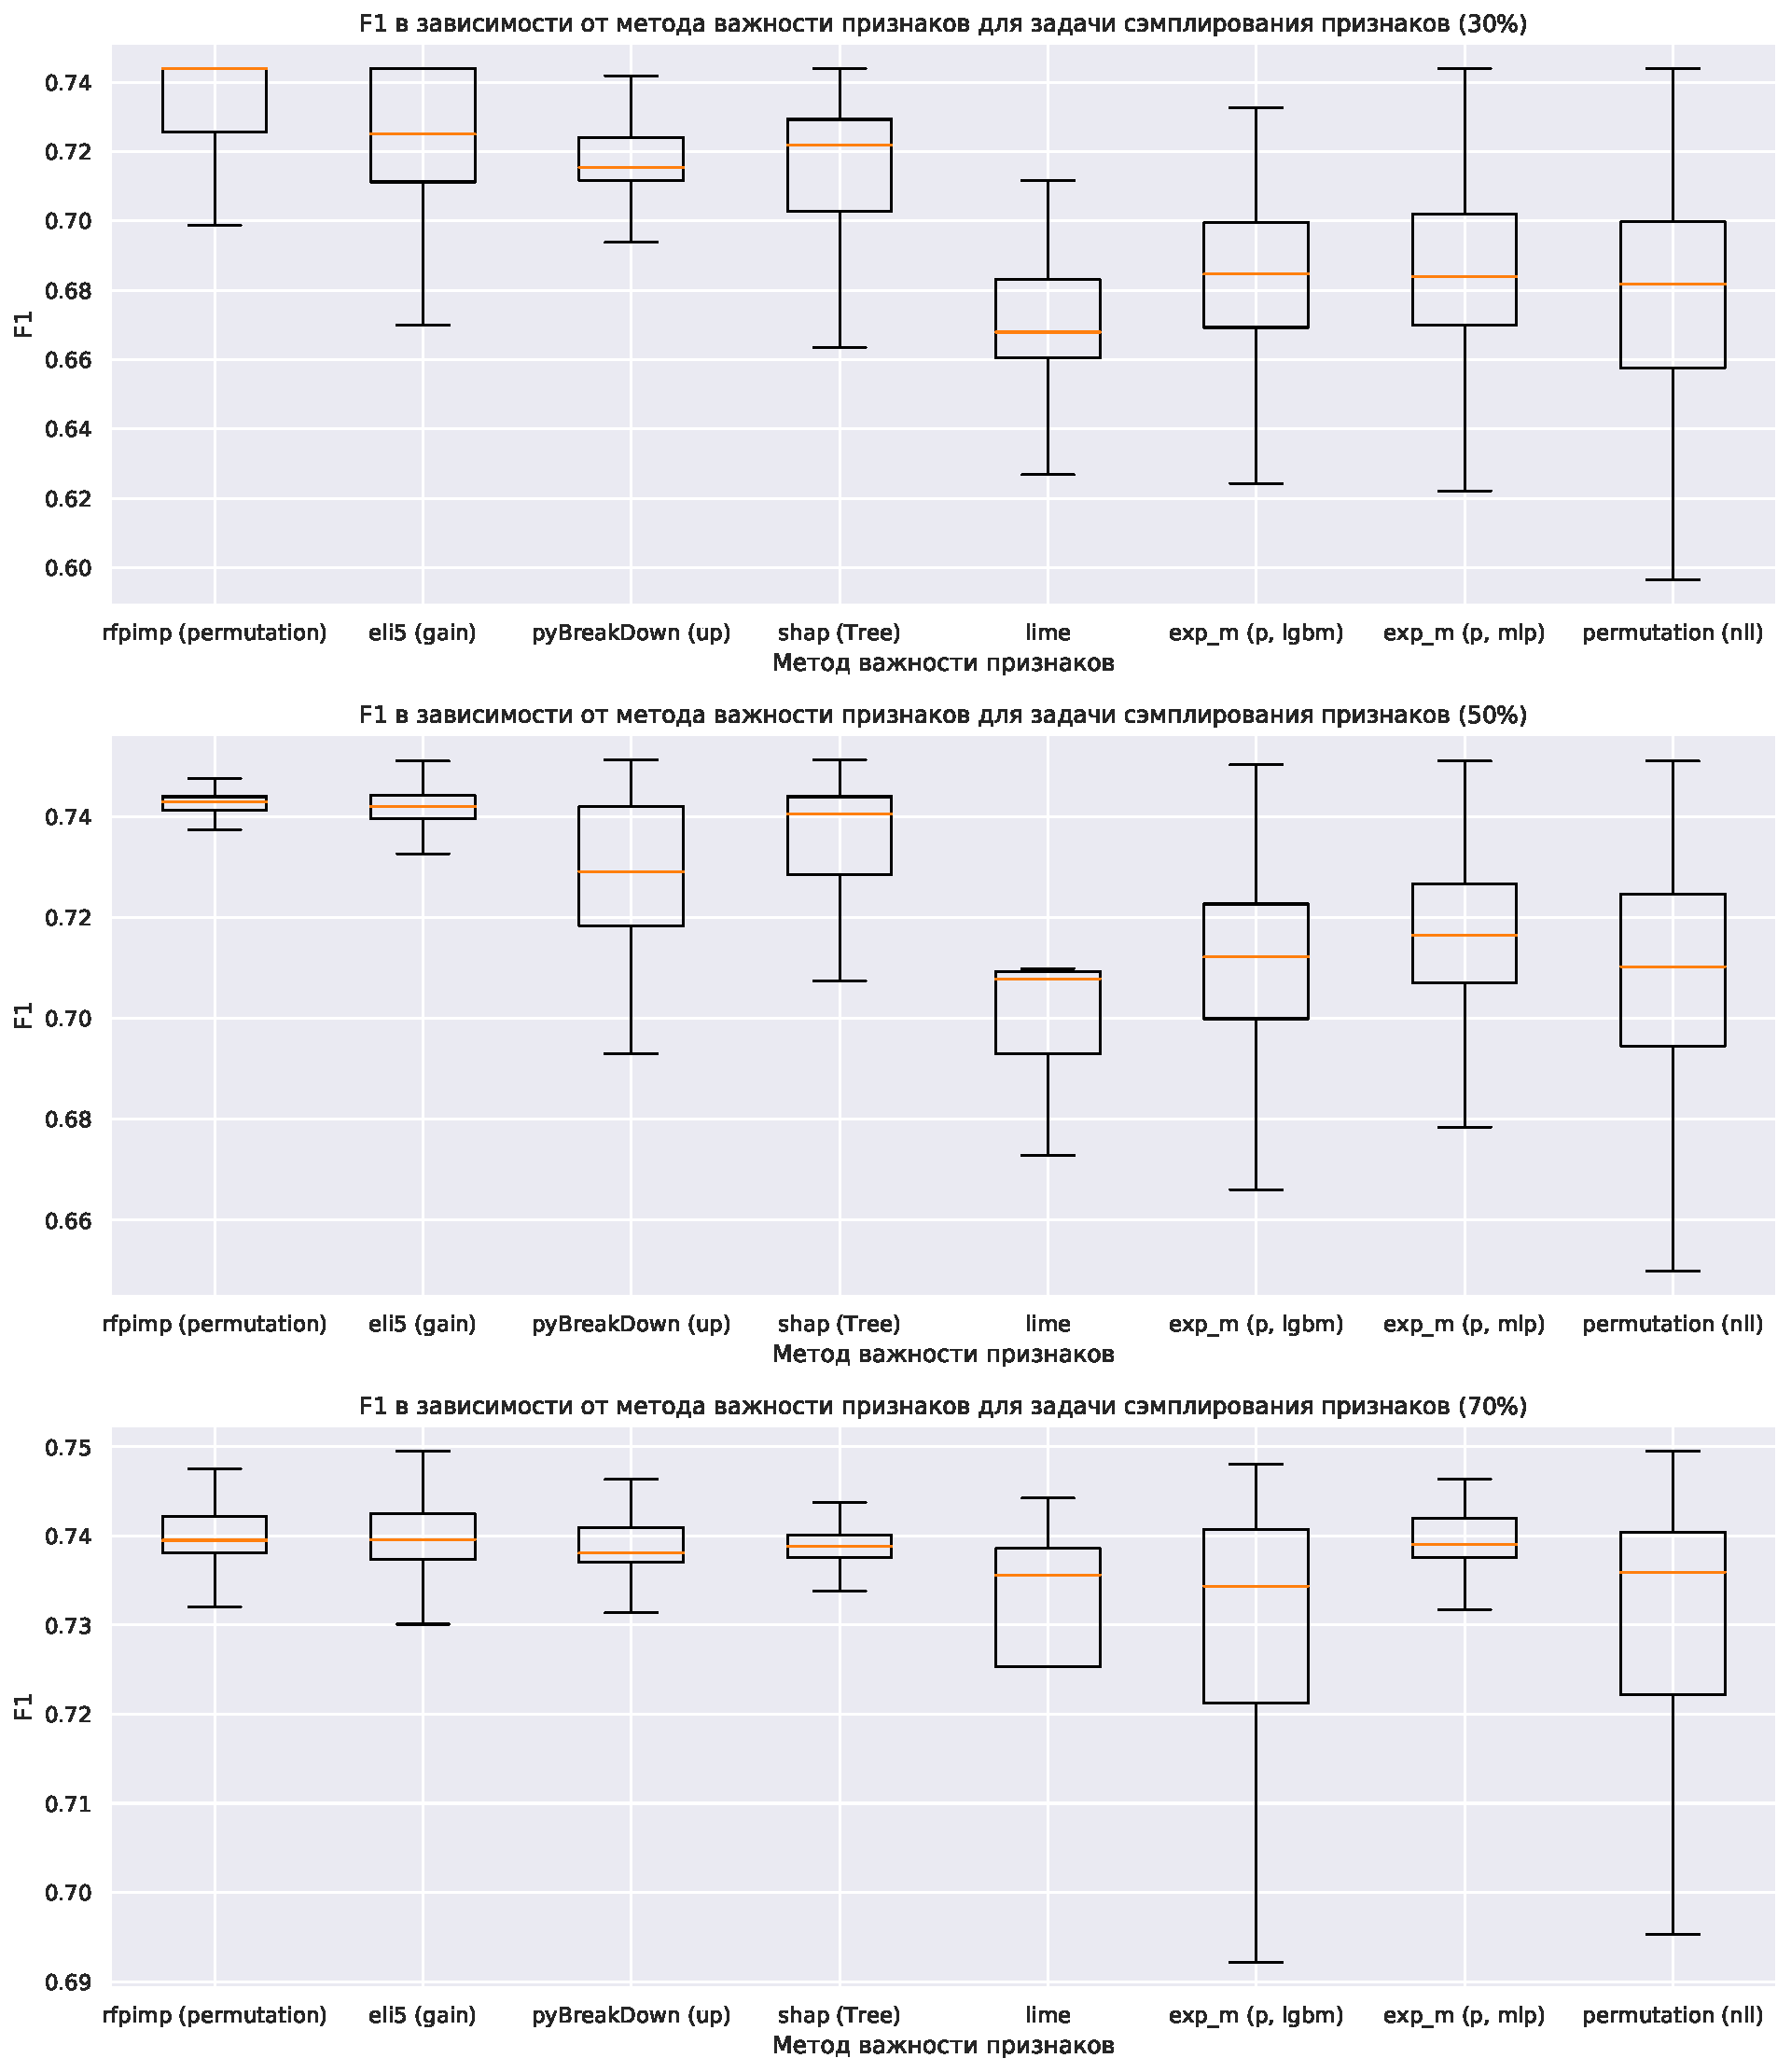
\includegraphics[width=\textwidth]{images/f1_feature_size.pdf}
% \caption{\centerin efw}
\end{figure}

При большом количестве признаков перестановочная, gain, pyBreakDown, shap, exp\_m(p, mlp) работают примерно одинаково. Однако при меньшем количестве признаков качество у pyBreakDown резко падает из--за итеративного алгоритма работы. Перестановочная важность (rfpimp) имеет лучшие результаты в целом.

\newpage
\subsubsection{Копия признака}
Выберем самый важный признак. Добавим его копию. На каждой итерации будем удалять наименее важный признак, за исключением выбранного и его копии. Обучать заново модель и повторять процедуру по достижению определенного количества оставшихся признаков
\begin{figure}[h]
        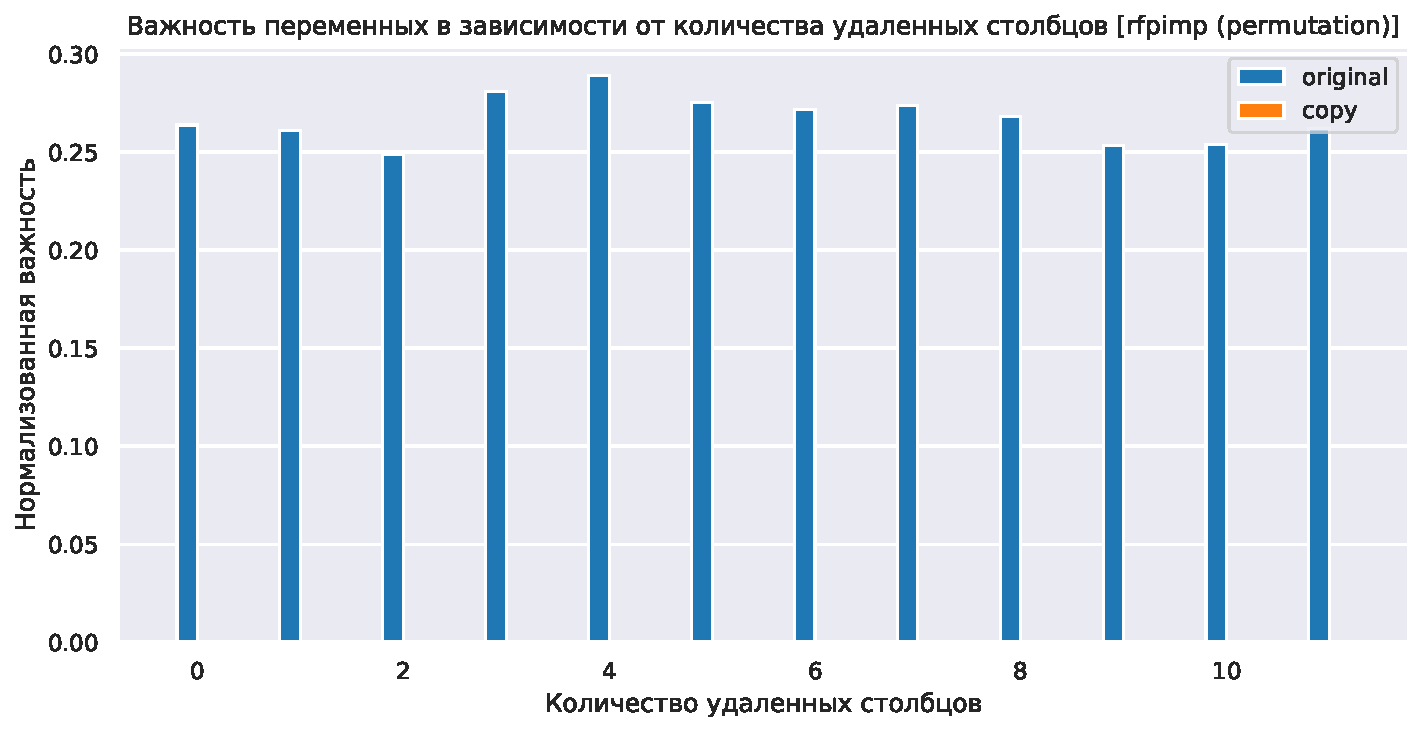
\includegraphics[width=0.5\textwidth]{images/art1_original_copy_lgbm_rfpimp (permutation).pdf}
        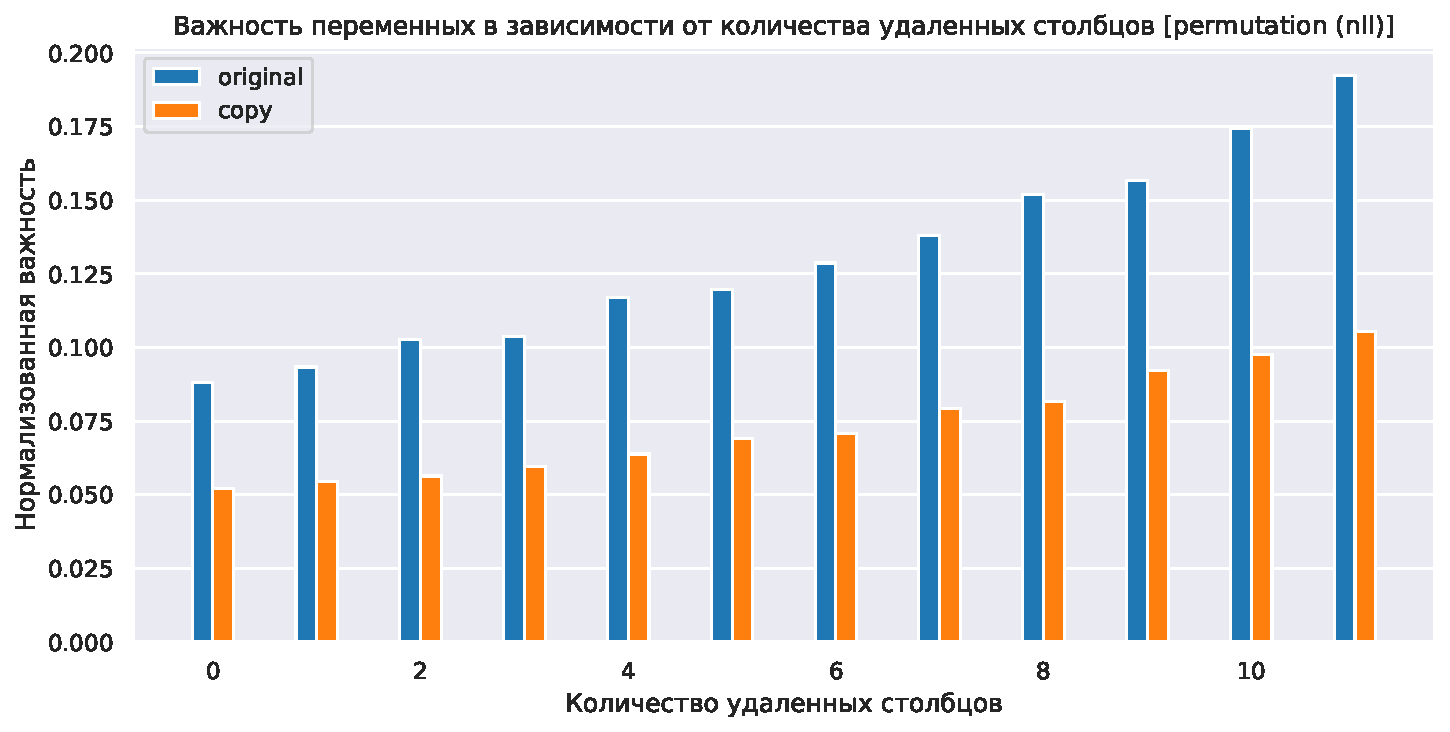
\includegraphics[width=0.5\textwidth]{images/art1_original_copy_lgbm_permutation (nll).pdf}
        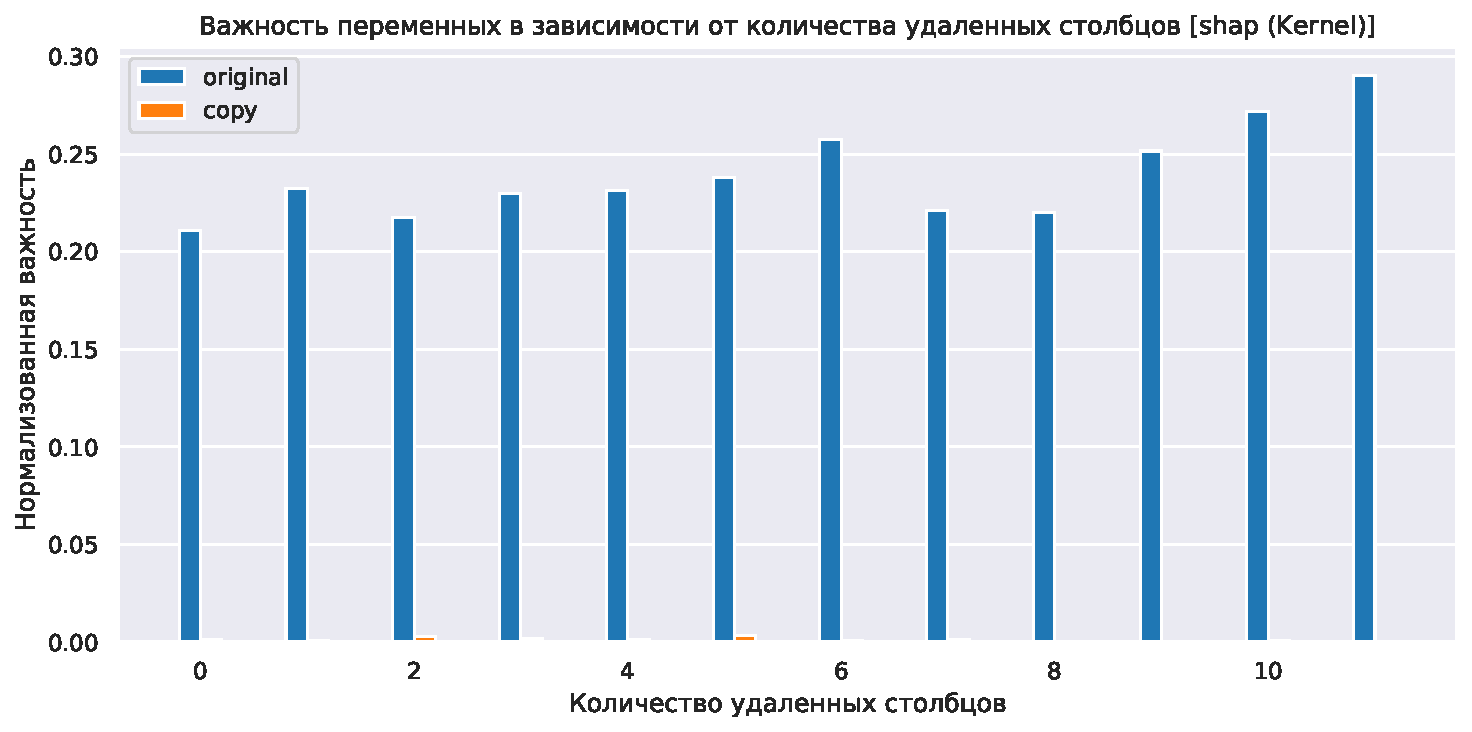
\includegraphics[width=0.5\textwidth]{images/art1_original_copy_lgbm_shap (Kernel).pdf}
        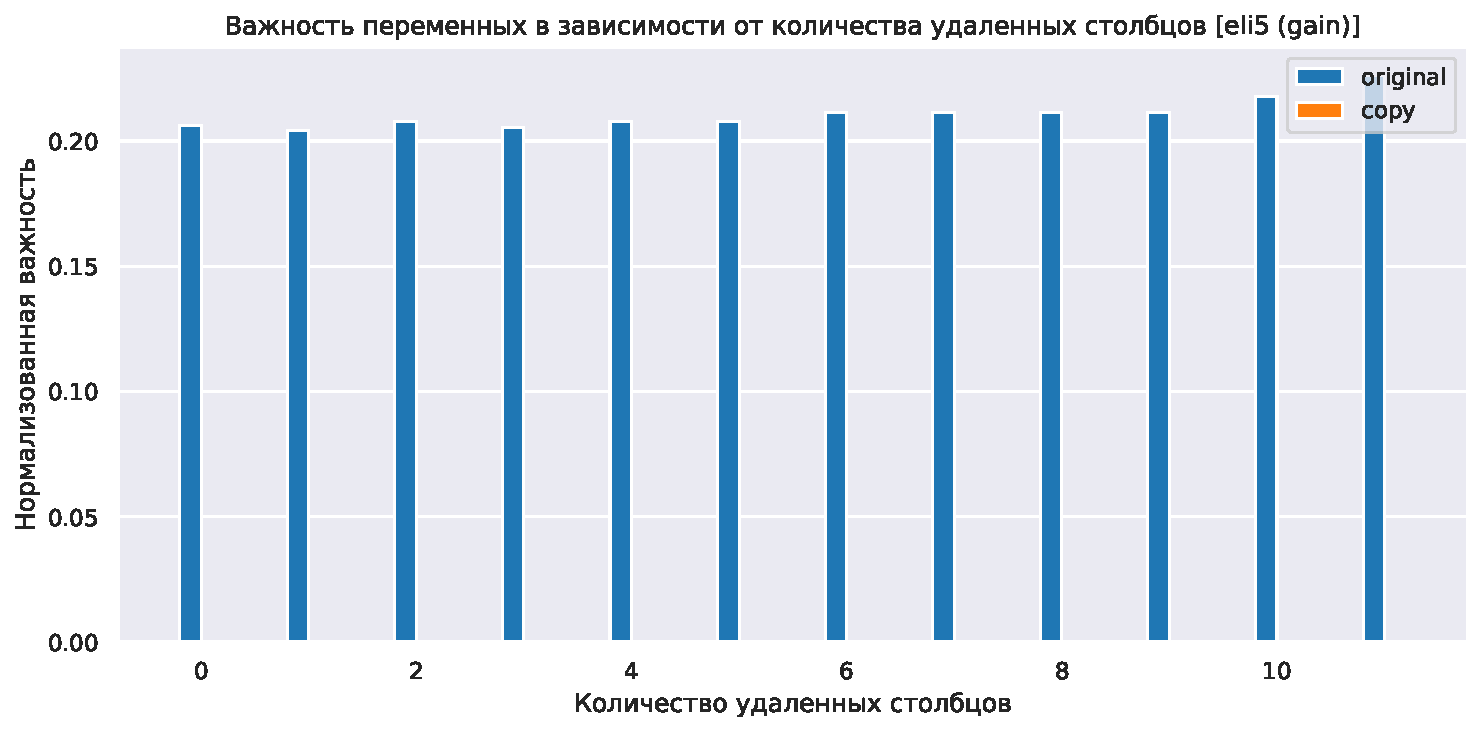
\includegraphics[width=0.5\textwidth]{images/art1_original_copy_lgbm_eli5 (gain).pdf}
        \hfill
        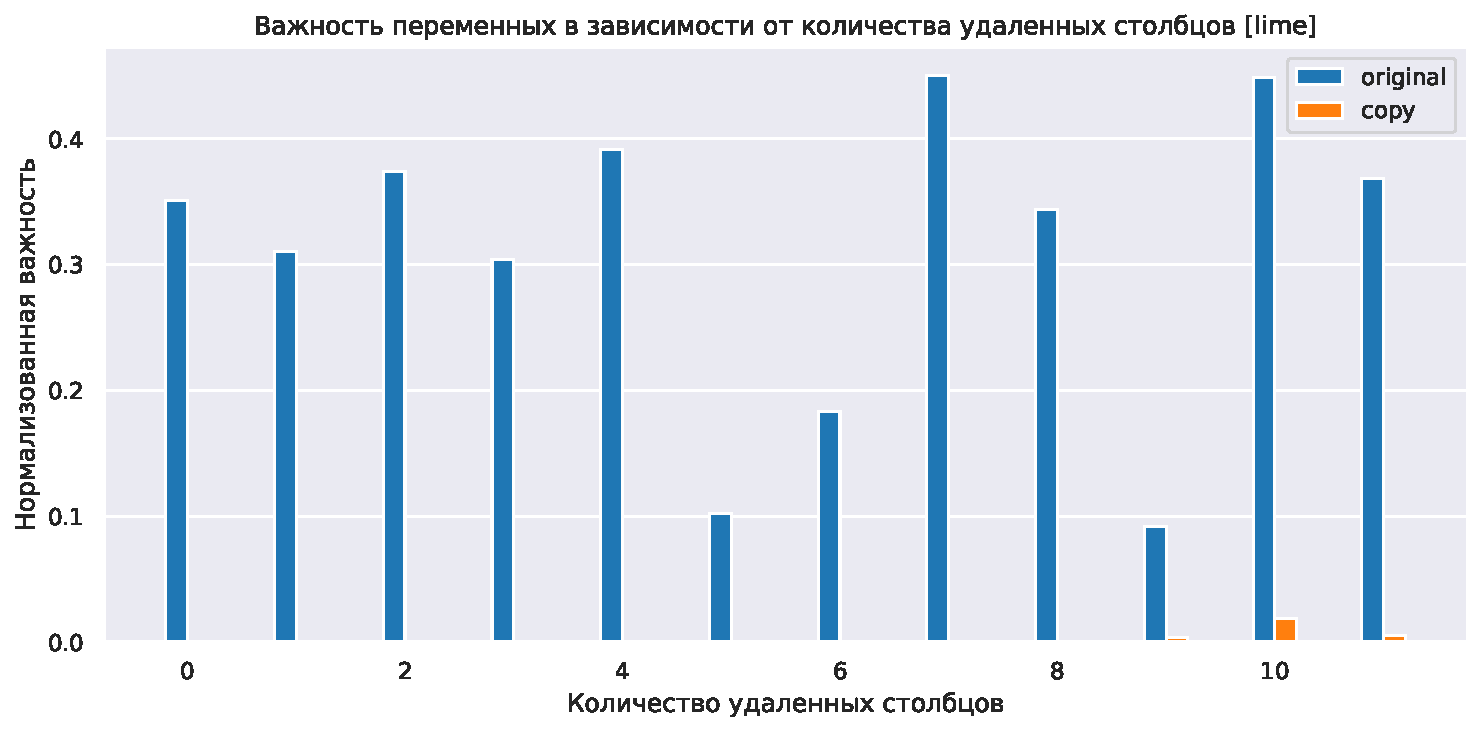
\includegraphics[width=0.5\textwidth]{images/art1_original_copy_lgbm_lime.pdf}
        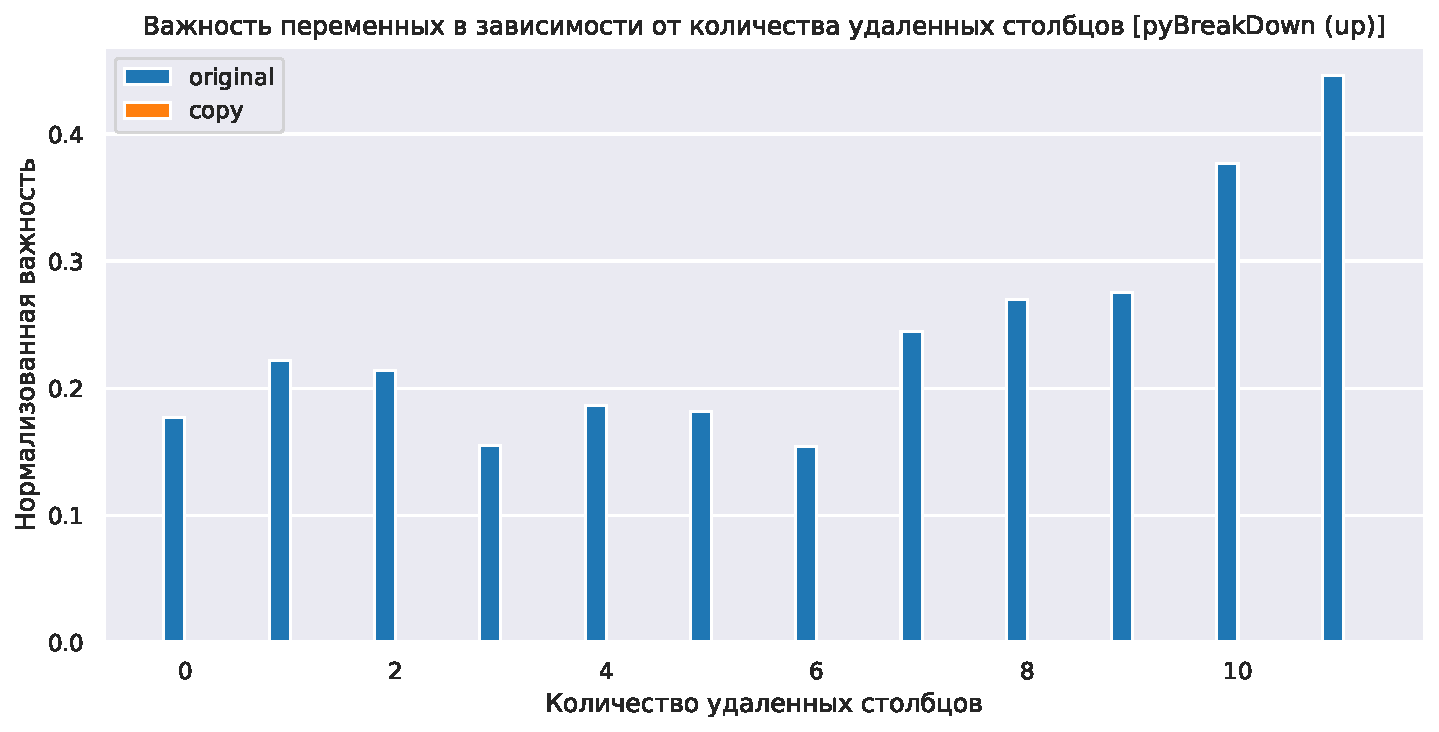
\includegraphics[width=0.5\textwidth]{images/art1_original_copy_lgbm_pyBreakDown (up).pdf}
        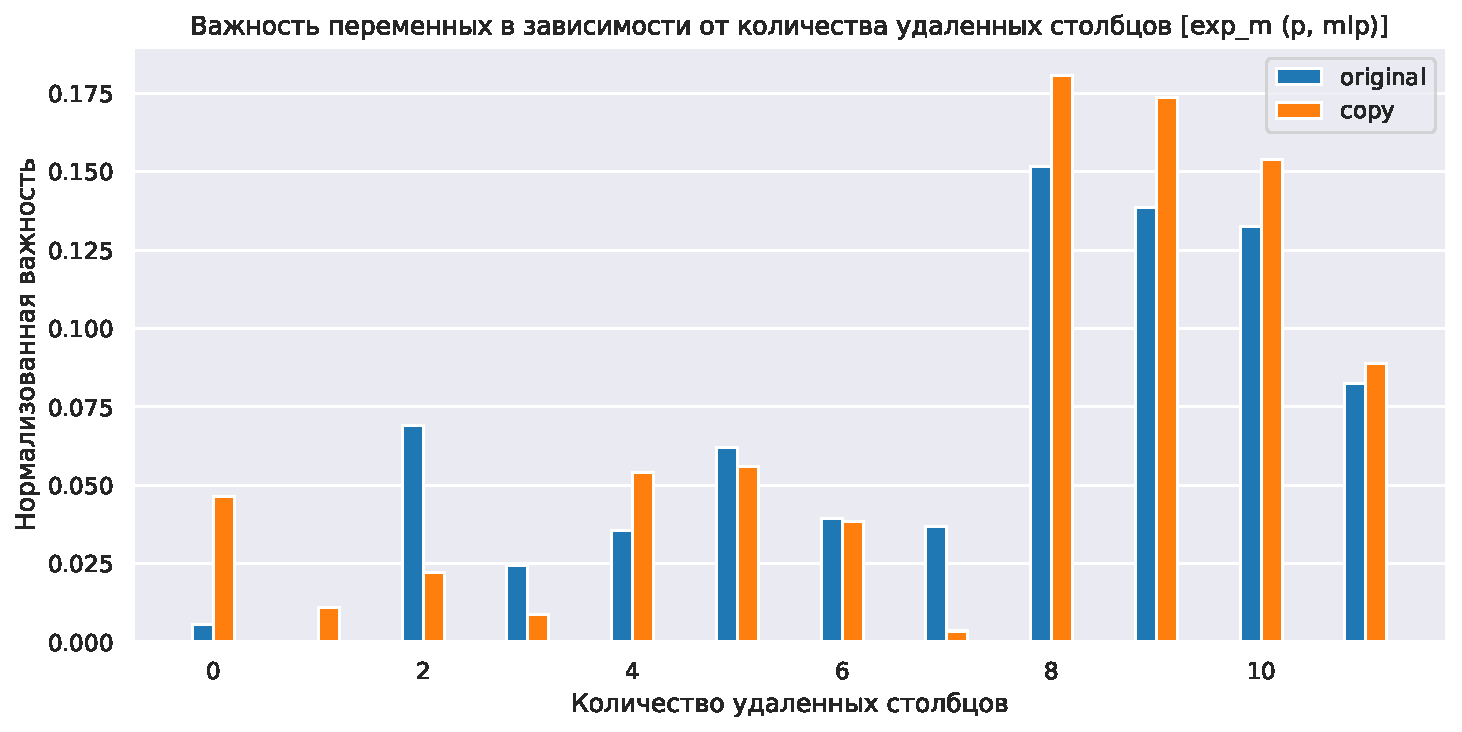
\includegraphics[width=0.5\textwidth]{images/art1_original_copy_lgbm_exp_m (p, mlp).pdf}
        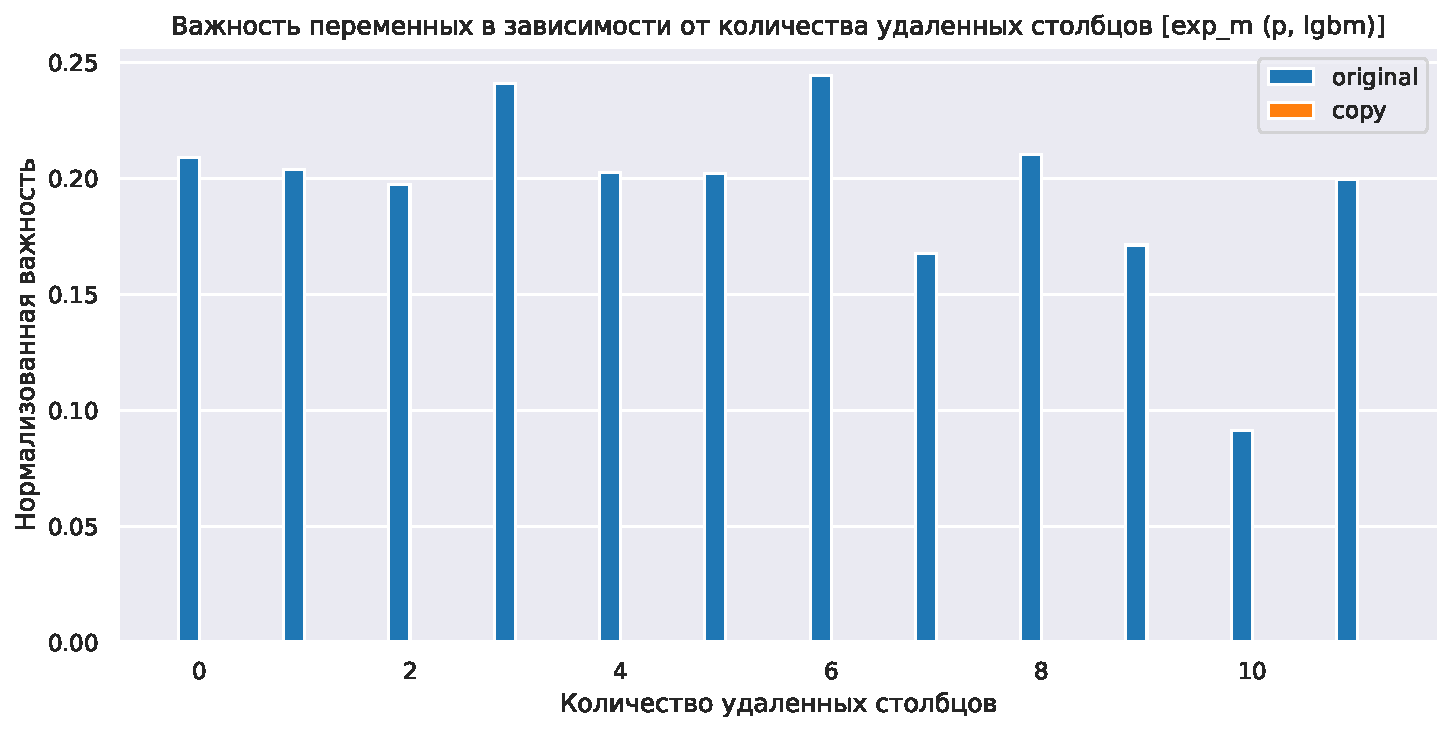
\includegraphics[width=0.5\textwidth]{images/art1_original_copy_lgbm_exp_m (p, lgbm).pdf}
\caption{\centering Исходная модель LGBM. Конечное количество признаков= 30\% от исходного. Для сэмплирования shap использовалось 100 объектов.}
\end{figure}

В большинстве случаев деревья не берут копию в качестве признака для разделения данных. Как следствие, значение копии равняется нулю. Однако с точки зрения (permutation (nll) вероятности положительного класса меняются.
\newpage
Возьмём SVM в качестве модели.
\begin{figure}[h]
        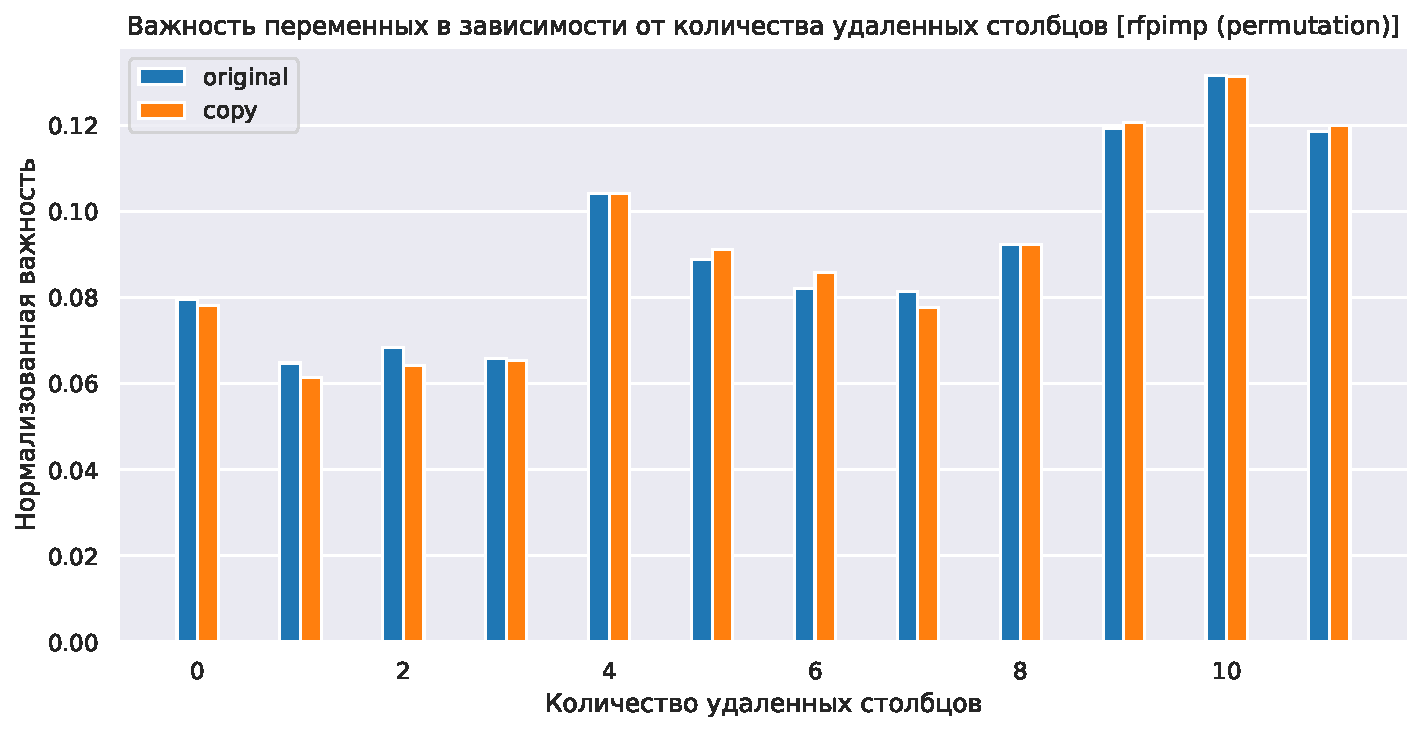
\includegraphics[width=0.5\textwidth]{images/art1_original_copy_svm_rfpimp (permutation).pdf}
        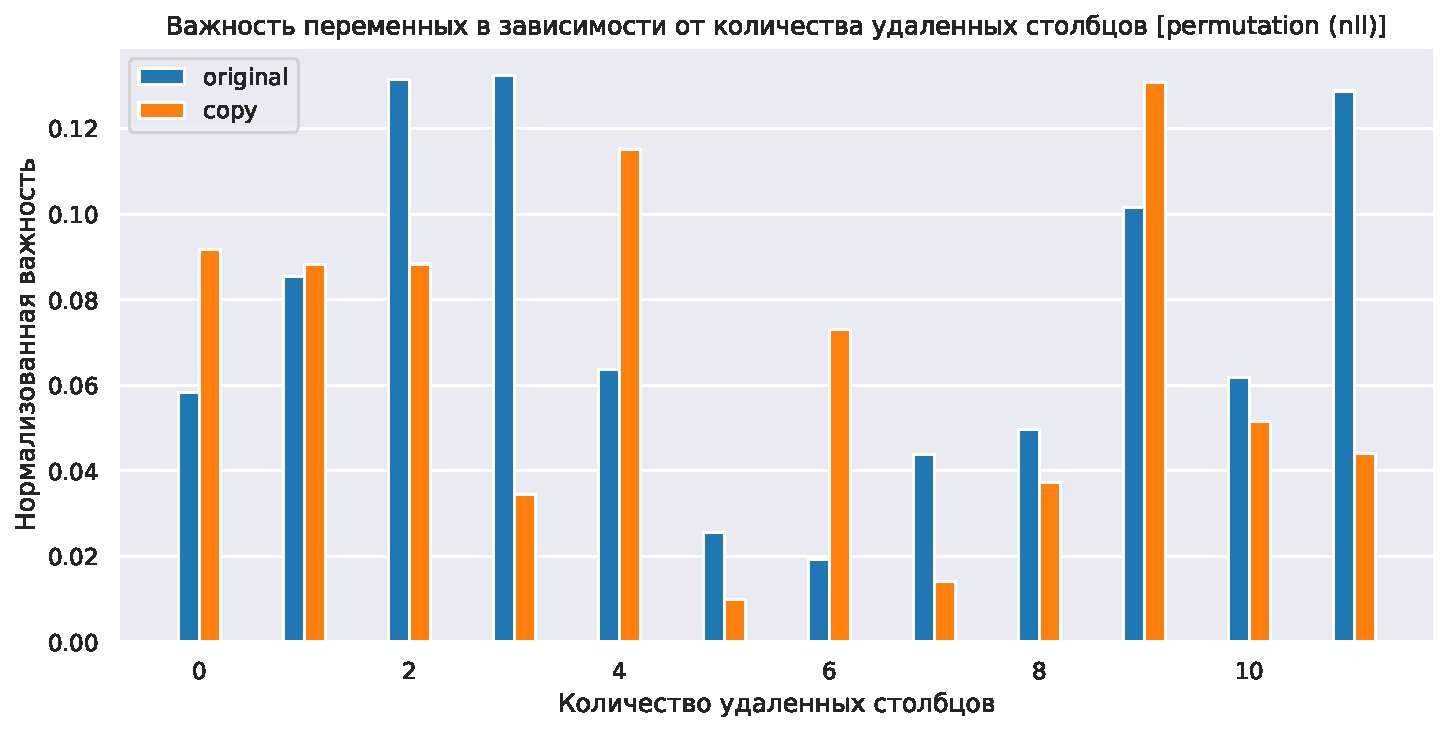
\includegraphics[width=0.5\textwidth]{images/art1_original_copy_svm_permutation (nll).pdf}
        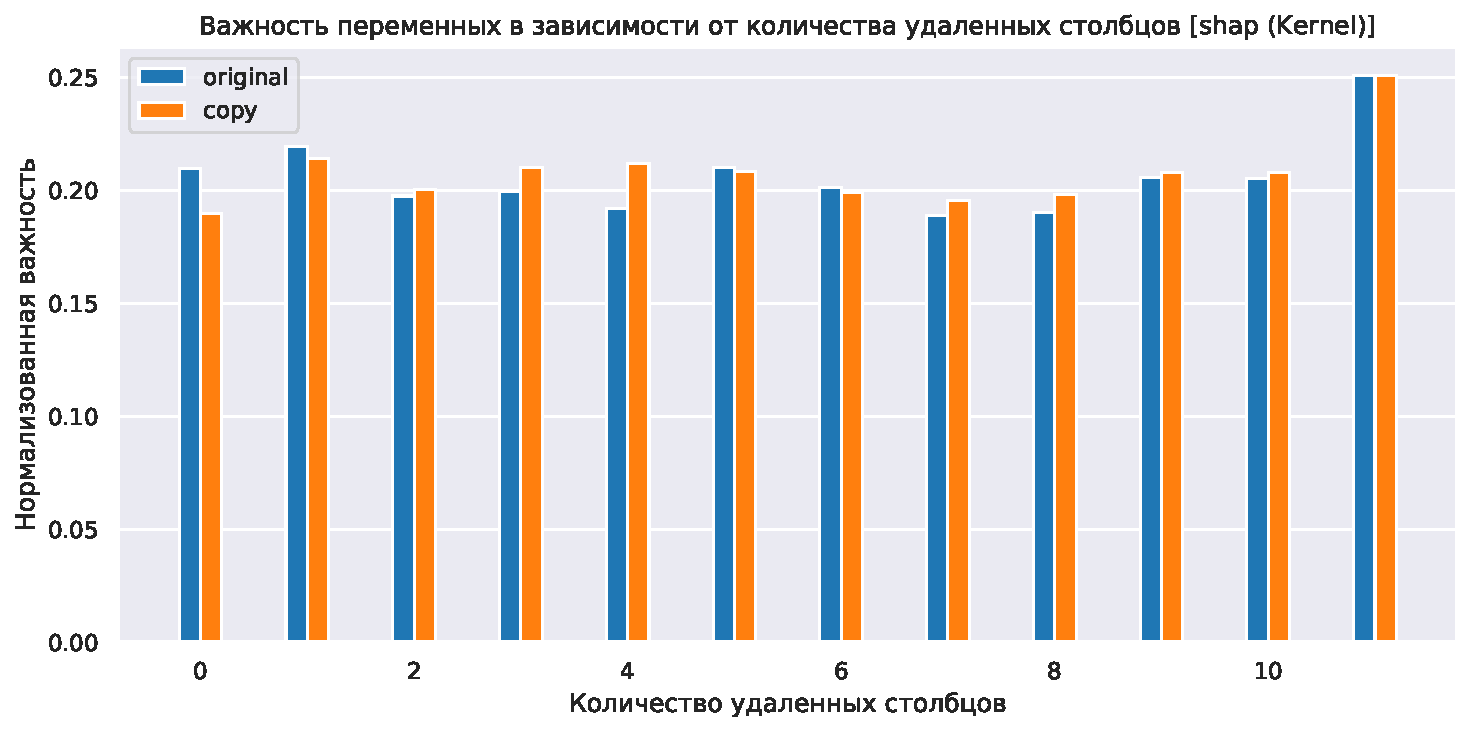
\includegraphics[width=0.5\textwidth]{images/art1_original_copy_svm_shap (Kernel).pdf}
        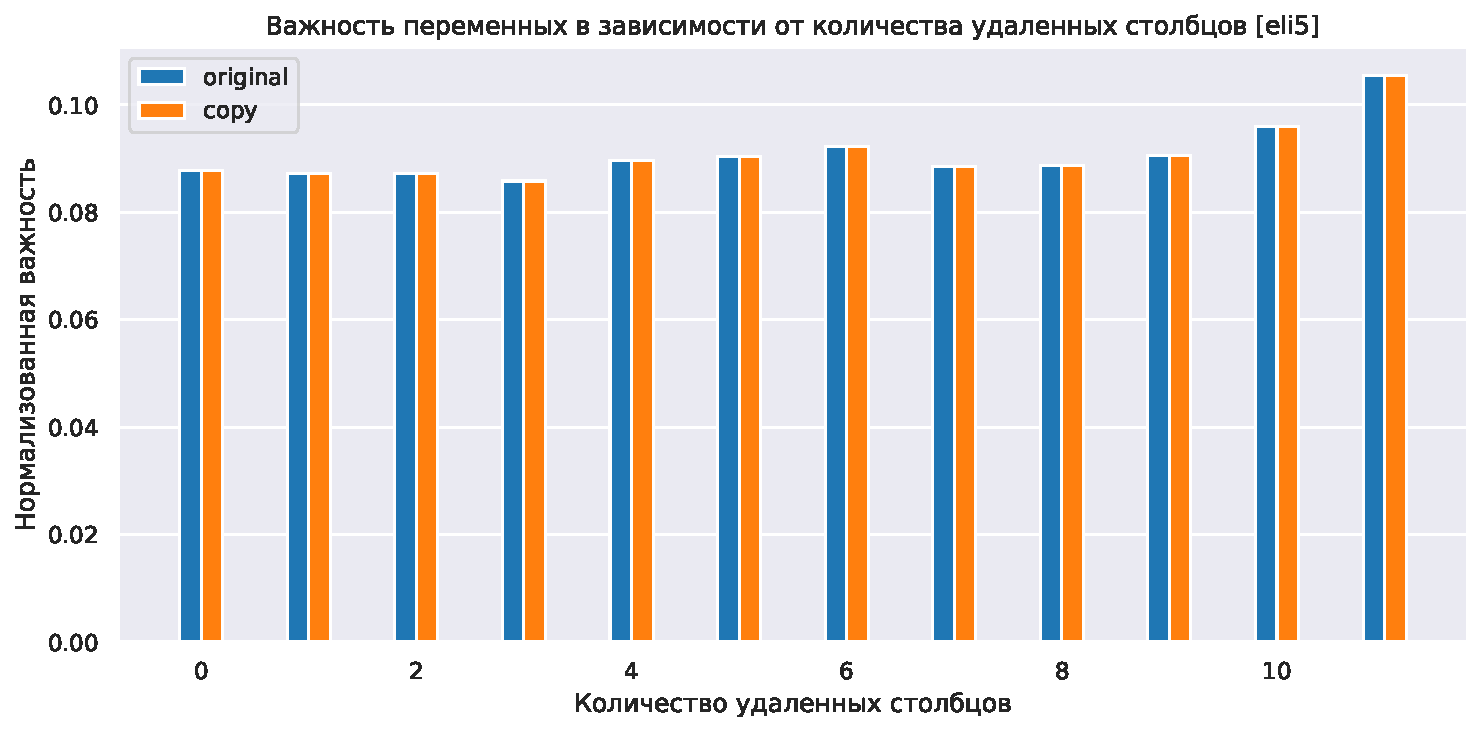
\includegraphics[width=0.5\textwidth]{images/art1_original_copy_svm_eli5.pdf}
        \hfill
        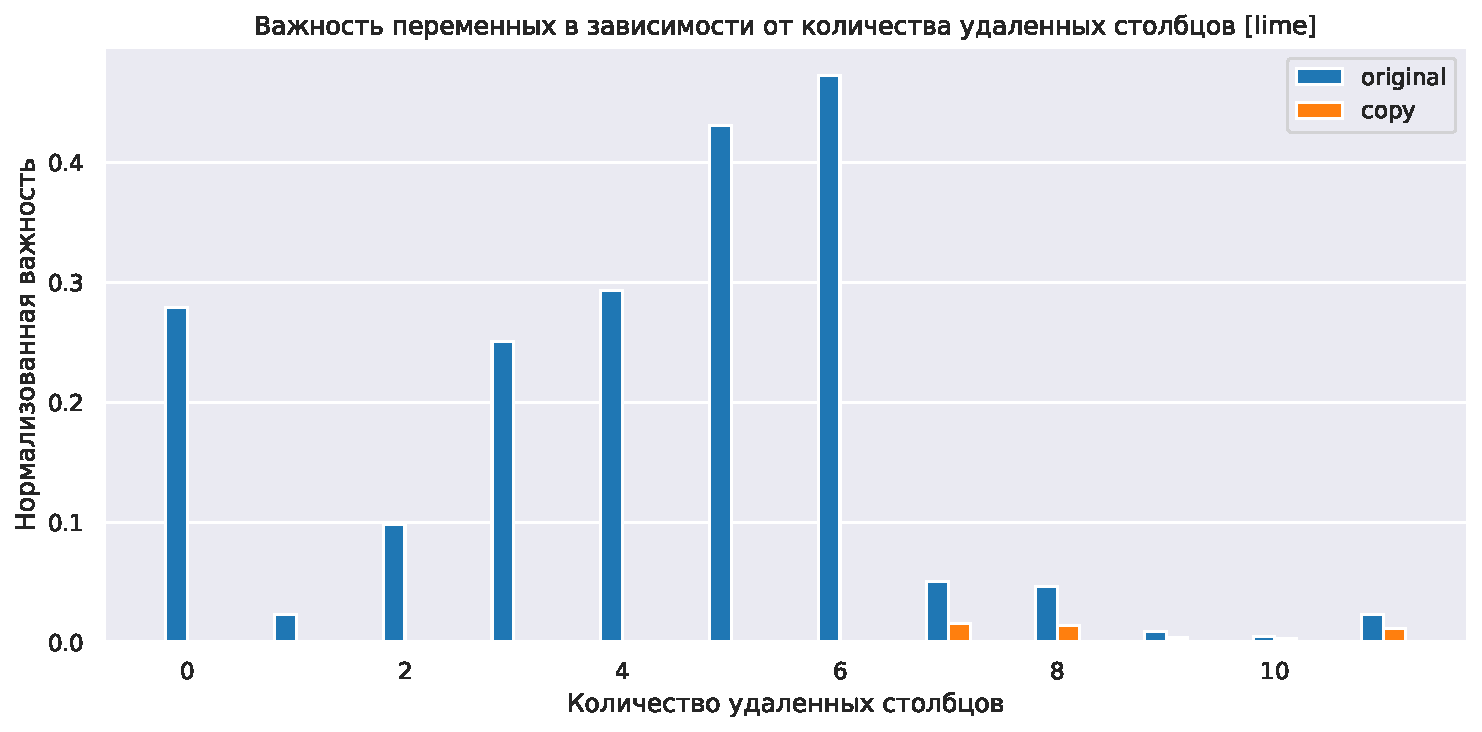
\includegraphics[width=0.5\textwidth]{images/art1_original_copy_svm_lime.pdf}
        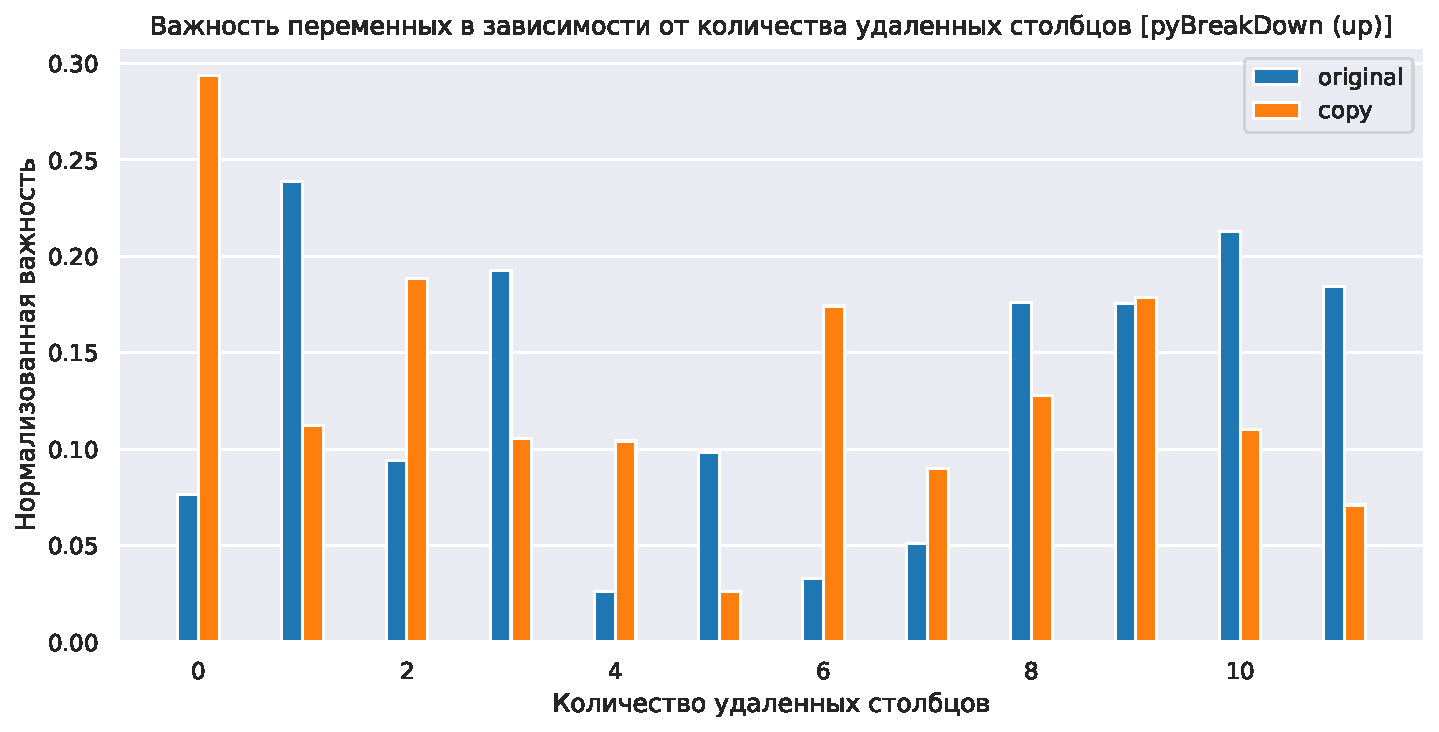
\includegraphics[width=0.5\textwidth]{images/art1_original_copy_svm_pyBreakDown (up).pdf}
        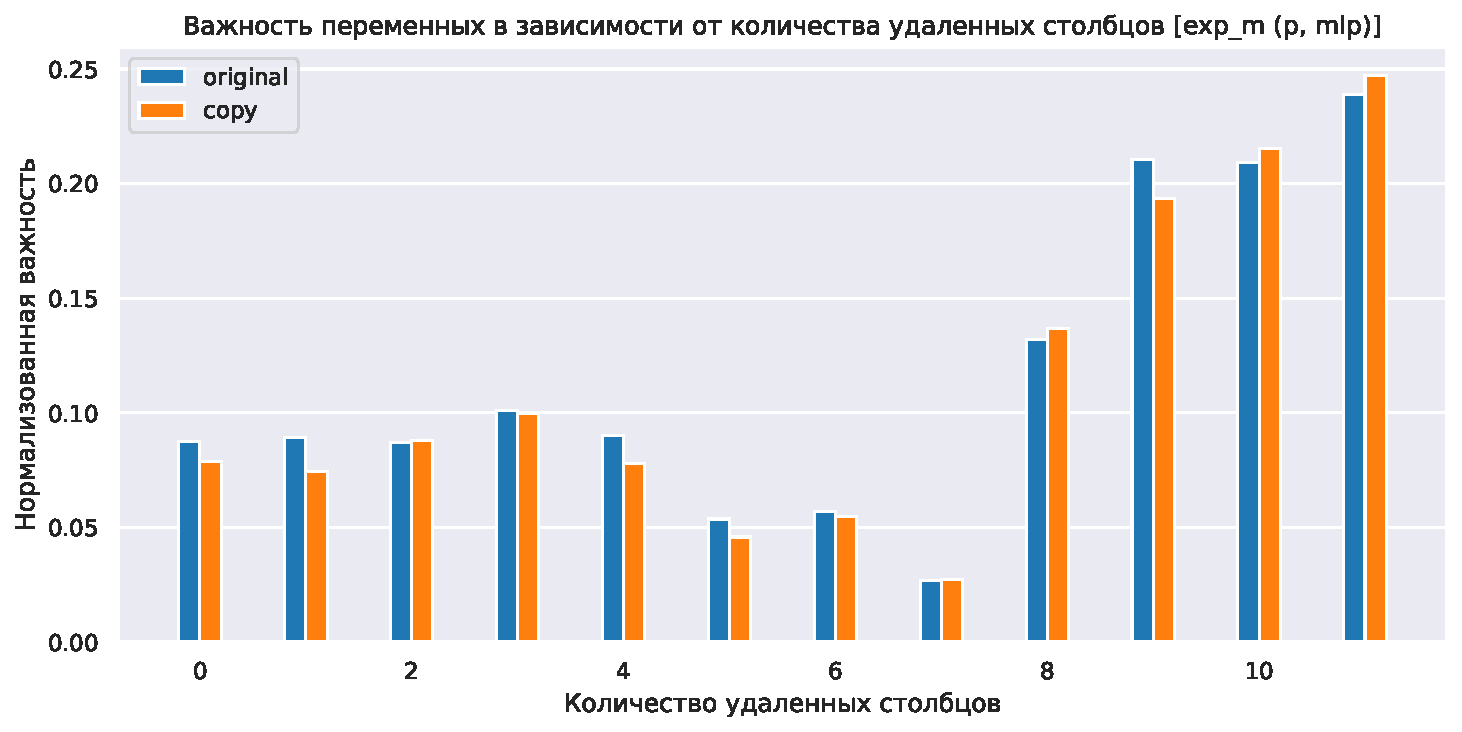
\includegraphics[width=0.5\textwidth]{images/art1_original_copy_svm_exp_m (p, mlp).pdf}
        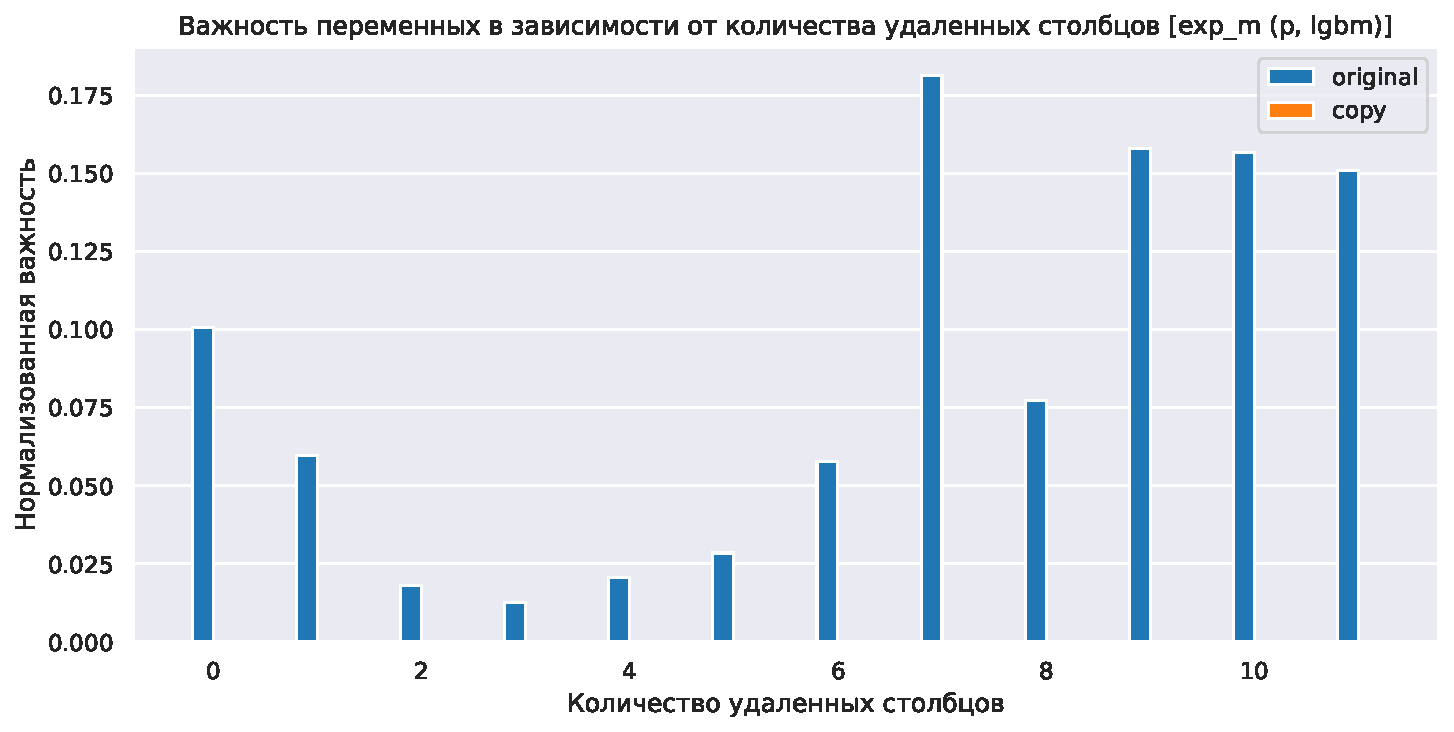
\includegraphics[width=0.5\textwidth]{images/art1_original_copy_svm_exp_m (p, lgbm).pdf}
\caption{\centering Исходная модель SVM. Конечное количество признаков= 30\% от исходного. Для сэмплирования shap использовалось 100 объектов.}
\end{figure}

Симметричные важности дают rfpimp, eli5, shap, exp\_m (p, mlp). Если выбирать данные методы, как способ фильтрации нужных переменных для предсказания, стоит обращать внимание на признаки, похожие друг на друг. Так как деление важности среди группы очень близких по значениям признаков скроет истинную оценку важности. Решением проблемы может стать выполнение иерархической кластеризации на основе ранговой корреляции Спирмена, выбор порога и сохранение одного признака из каждого кластера. 

Использование линейного слоя нейронной сети в качестве объясняющей модели помогло избавиться от асимметричного распределения важности. 

\newpage
\subsection{Функции}
Рассмотрим некоторые простые функции от многих переменных.
\subsubsection{Данные}
Признаки $X_1, ... , X_6, eps$ связаны с $Y$ следующим образом:
\begin{gather*}
    Y_{r e g}=X_{1} X_{2} X_{3}+X_{4}+X_{5}+X_{6}+e p s, \hspace{1em}\text { где } e s p \sim N\left(0,0.1^{2}\right), X_{i} \sim N(0,1)\\
    Y_{c l f}= \mathbb{I}[Z \geq \operatorname{median}(Z)], \hspace{1em}\text{где} \, Z = \sigma\left(Y_{r e g}-\operatorname{mean}\left(Y_{r e g}\right)\right)
\end{gather*}
Количество сэмплированных объектов равно 1000.
В качестве модели использовался бустинг (LightGBM).

\subsubsection{Стандартная классификация/регрессия}
\begin{figure}[h]
\centering
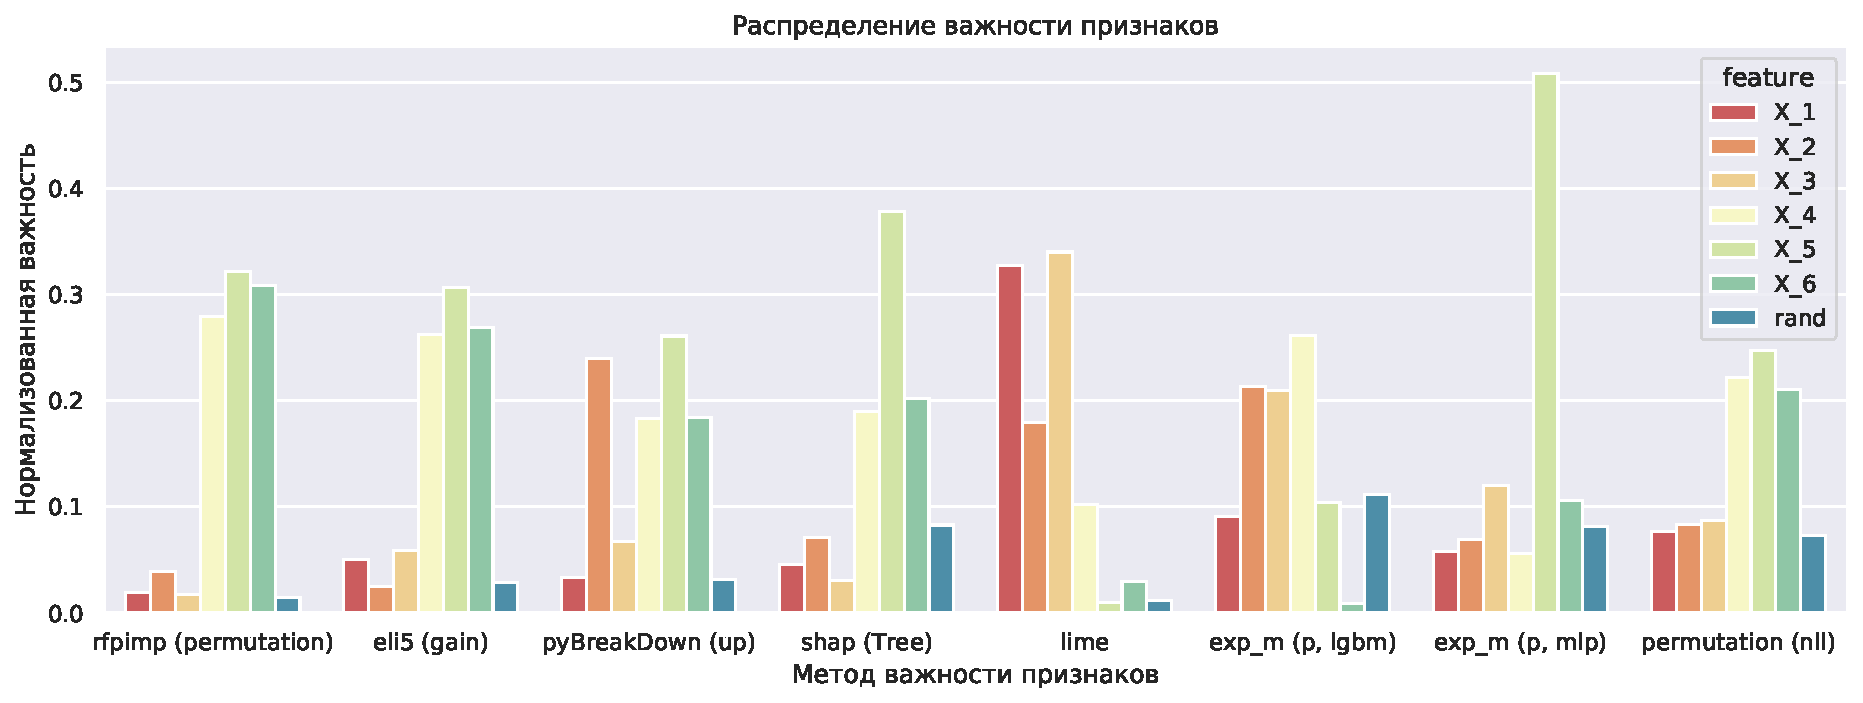
\includegraphics[width=\textwidth]{images/at2_setup1.pdf}
\caption{$y=y_{clf}$}
\end{figure}

\begin{figure}[h]
\centering
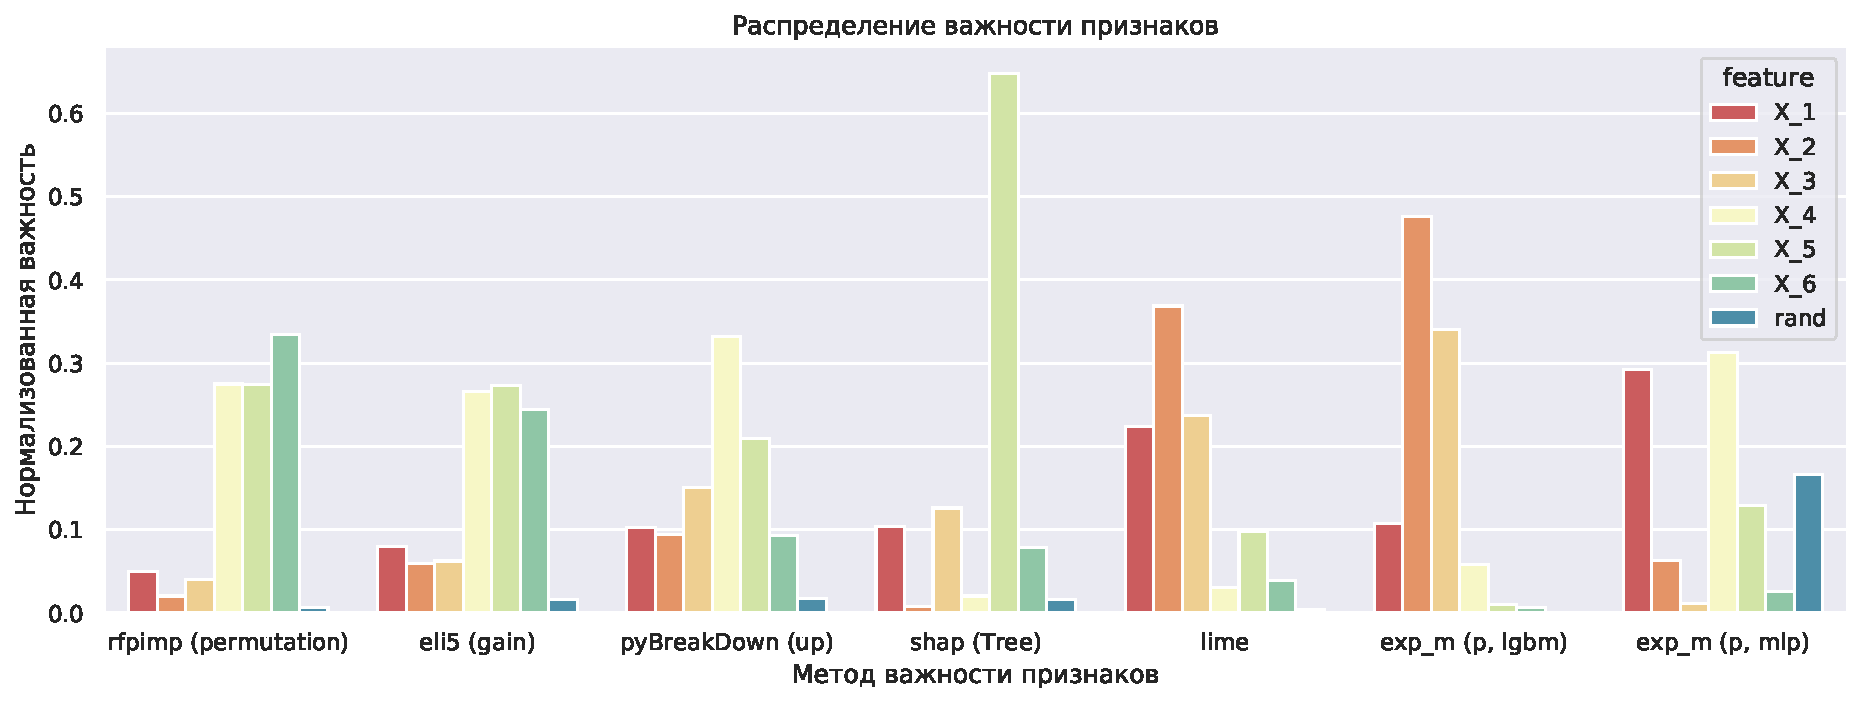
\includegraphics[width=\textwidth]{images/at2_setup3.pdf}
\caption{$y=y_{reg}$}
\end{figure}

Наименьшую важность случайному признаку дает rfpimp, lime. Перестановочная важность отдает предпочтение более независимым признакам: $X_4, X_5, X_6$. Более того, сумма важностей $X_1, X_2, X_3$ не равняется важности $X_4$, или $X_5$, или $X_6$. Это говорит о том, что признаки участвующие в сложных взаимосвязях могут получить маленькую оценку важности.
% Это говорит о том, что признаки, участвующие во взаимодействии большого порядка, например, в нейросетях, будут занижаться в оценке важности.

\newpage
\subsubsection{Квадратичная функция}
\begin{figure}[h]
\centering
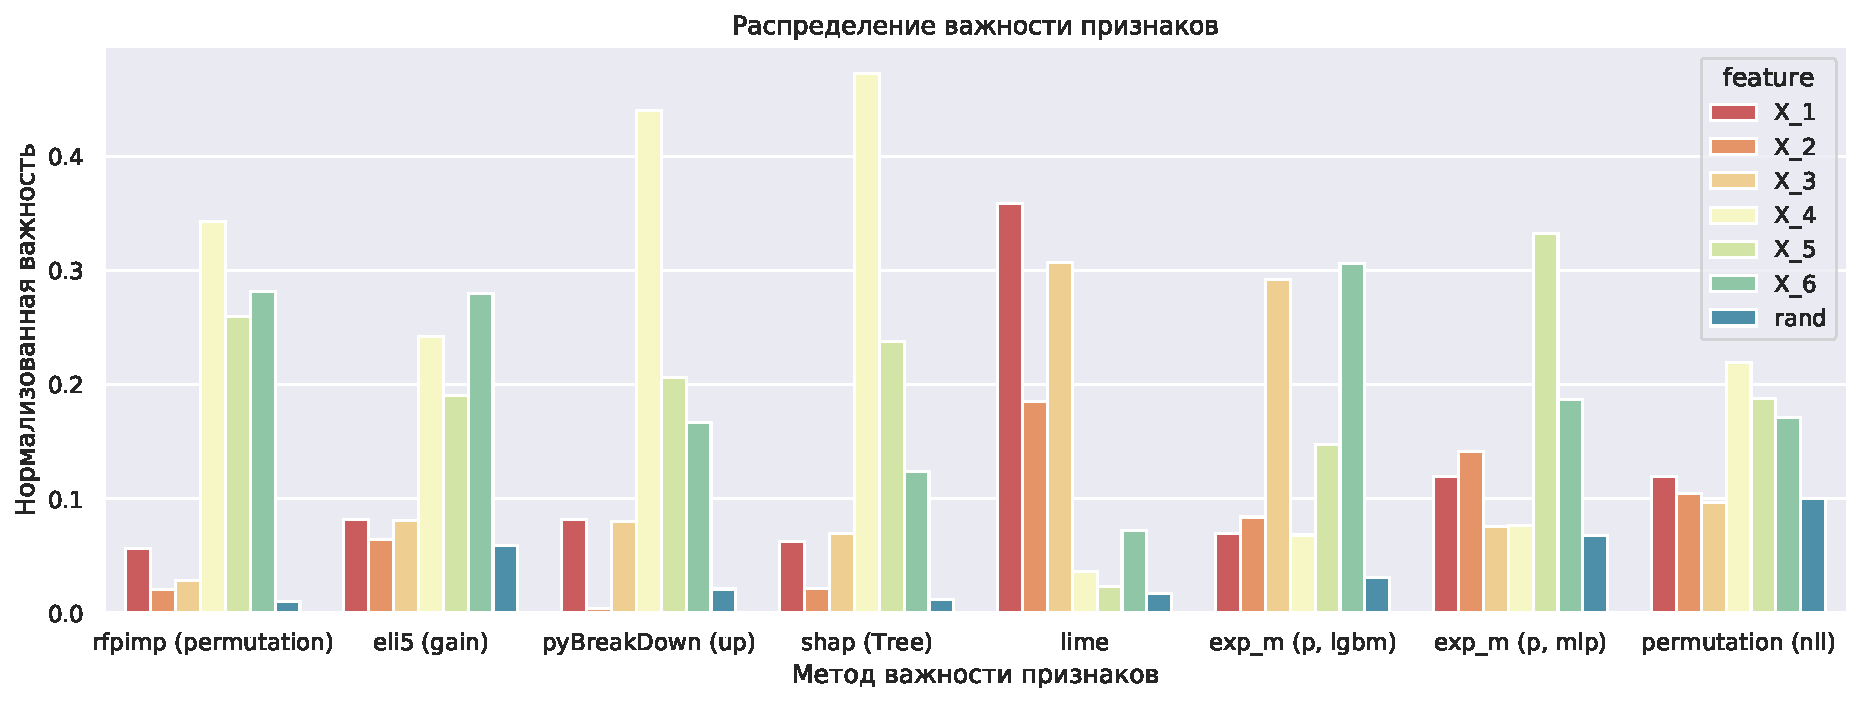
\includegraphics[width=\textwidth]{images/at2_setup2.pdf}
\caption{$y=y_{clf}\left(y_{\text {reg }}^{2}\right)$}
\end{figure}

\begin{figure}[h]
\centering
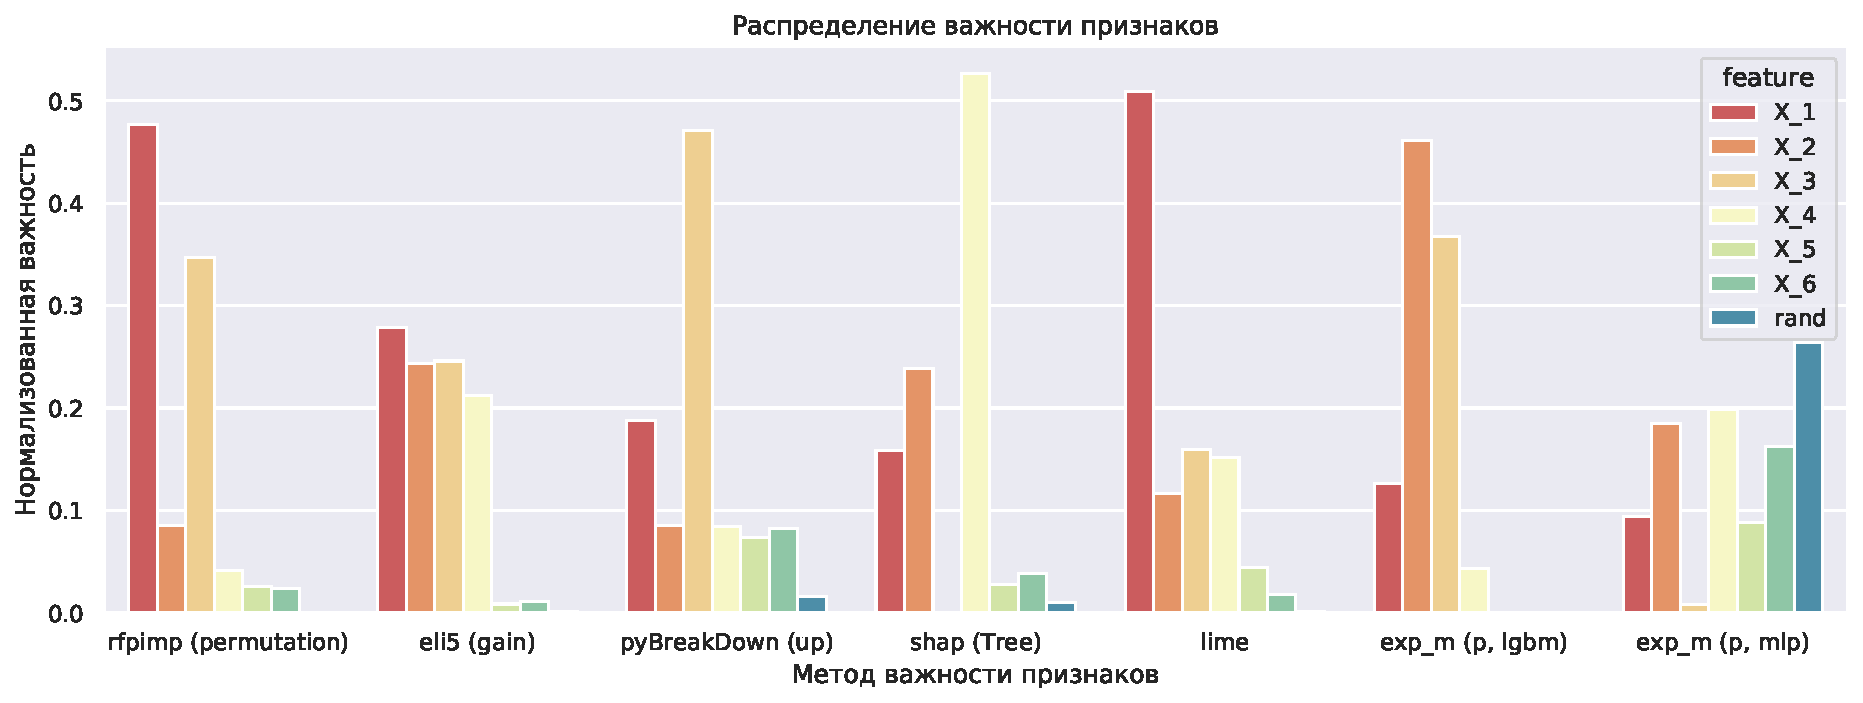
\includegraphics[width=\textwidth]{images/at2_setup4.pdf}
\caption{$y=y_{reg}^{2}$}
\end{figure}

Признаки $X_1, X_2, X_3$ сохранили свою важность для $y=y_{clf}\left(y_{\text {reg }}^{2}\right)$ из-за поведения сигмоиды на бесконечности: при относительно больших#/малых $z$, $\operatorname{sigmoid}(z)$ не сильно меняется. Для $y=y_{reg}^{2}$ же сигмоида не применялась.

\newpage
\subsubsection{Степенная функция}
\begin{figure}[h]
\centering
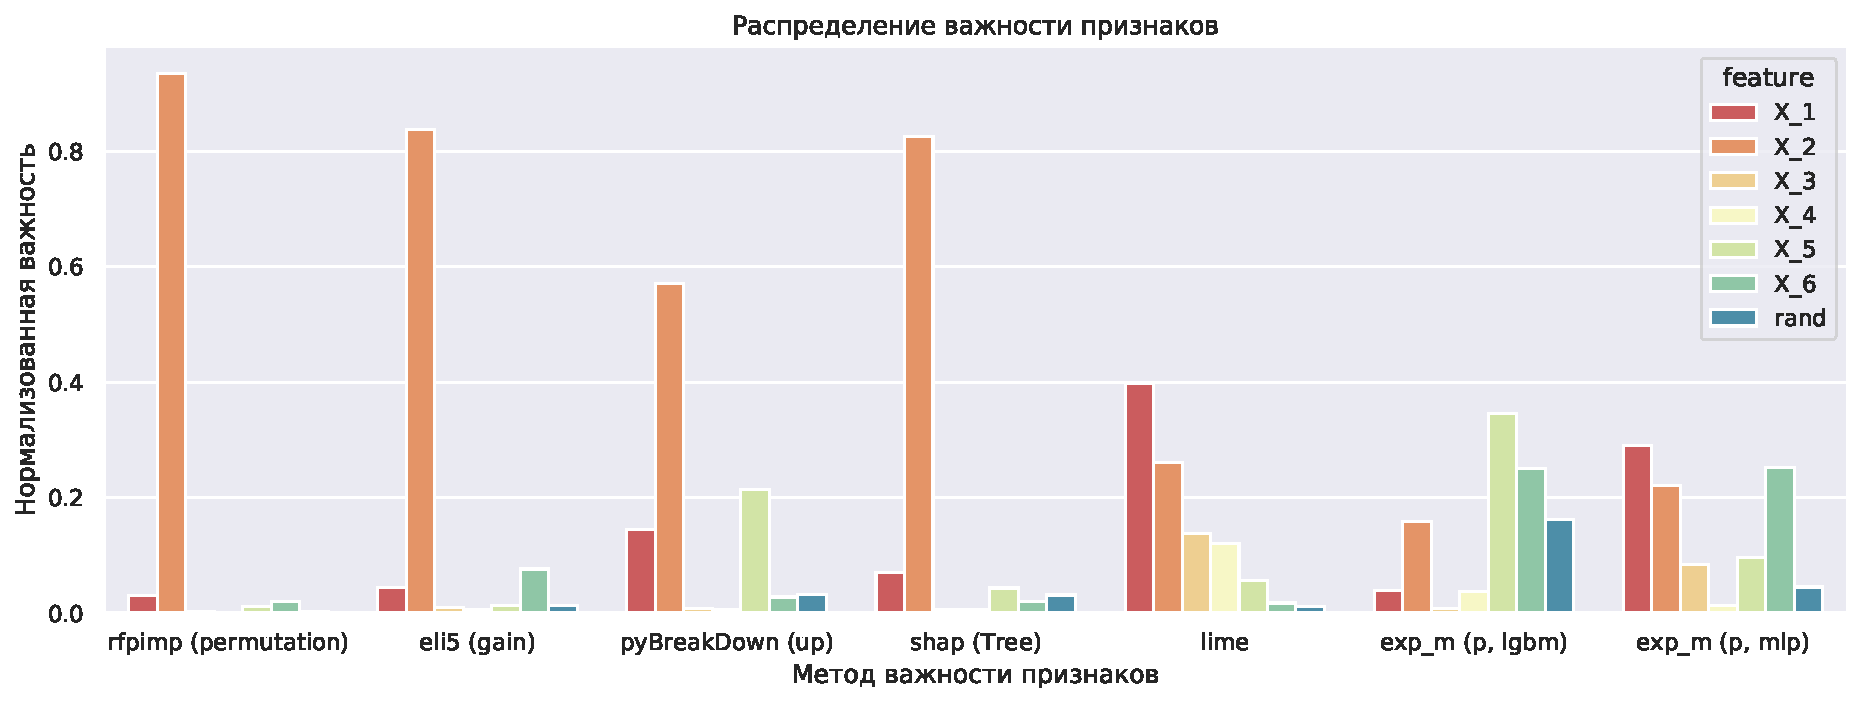
\includegraphics[width=\textwidth]{images/at2_setup5.pdf}
\caption{$y=\left|X_{1}+10\right|^{\left(X_{2}+10\right)}$}
\end{figure}

Lime плохо обобщает из--за предположения независимости признаков. В большинстве случаев признак при степени более важен. Важность с использованием объясняющей модели показала плохие результаты. Большую роль играет сложность объясняющей модели. В данном примере ее оказалось недостаточно.

\subsubsection{Сумма по модулю 2}
Здесь все признаки одинаково важны и задаются следующим образом:
\begin{gather*}
    X_{1}, \ldots, X_{6}, X_{7} \sim B i(1,0.5) \\
    y=\operatorname{Xor}\left(X_{1}, \ldots, X_{6}\right)
\end{gather*}
\begin{figure}[h]
\centering
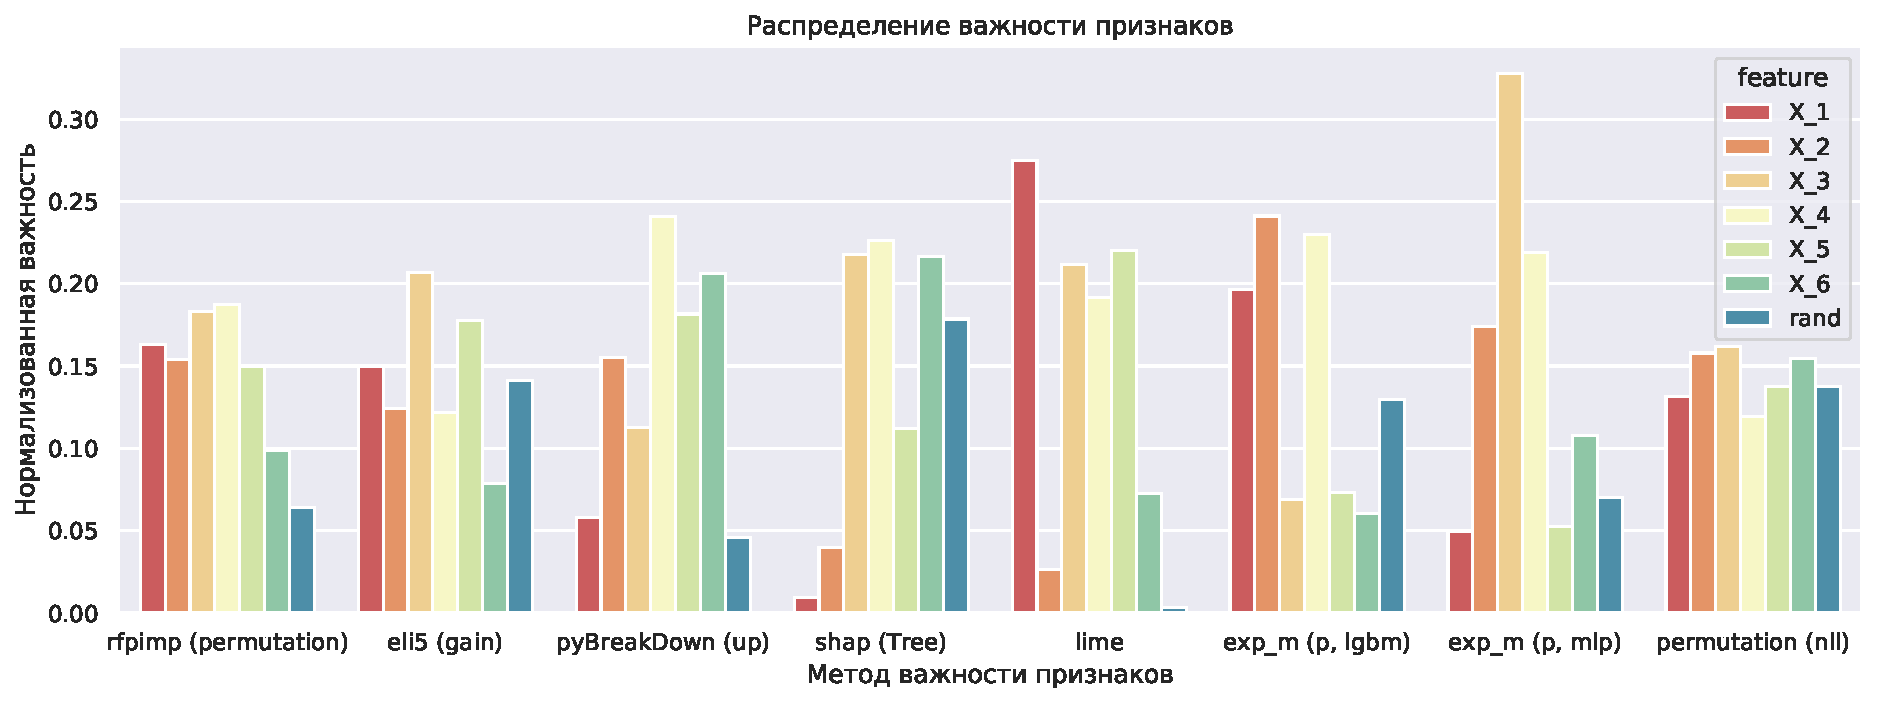
\includegraphics[width=\textwidth]{images/at2_setup6.pdf}
\end{figure}

Shap дает большую важность случайному признаку, так как в большом количестве подмножеств признаков является важным. Это может свидетельствовать о переобучении модели. Аналогичные рассуждения применимы и для permutation (nll). 

Если сравнивать оценки важностей признаков с оценкой для случайного признака, то перестановочная важность (f1) показала лучшие результаты.
\newpage
\subsection{Прогноз диабета}
\subsubsection{Данные}
Датасет был взят с \href{https://www.kaggle.com/uciml/pima-indians-diabetes-database}{сайта kaggle}. Признаки состоят из наиболее связанных с целевой меткой параметров: уровень глюкозы (Glucose), уровень инсулина (Insulin), функция родословного диабета (DiabetesPedigreeFunction) и так далее. Всего 9 штук. В качестве модели использовались бустинг (LightGBM) и метод опорных векторов (SVС).

Повторим эксперименты секции \ref{corr_expir}.

\subsubsection{Важность}\label{diab_imortance}

\begin{figure}[h]
\centering
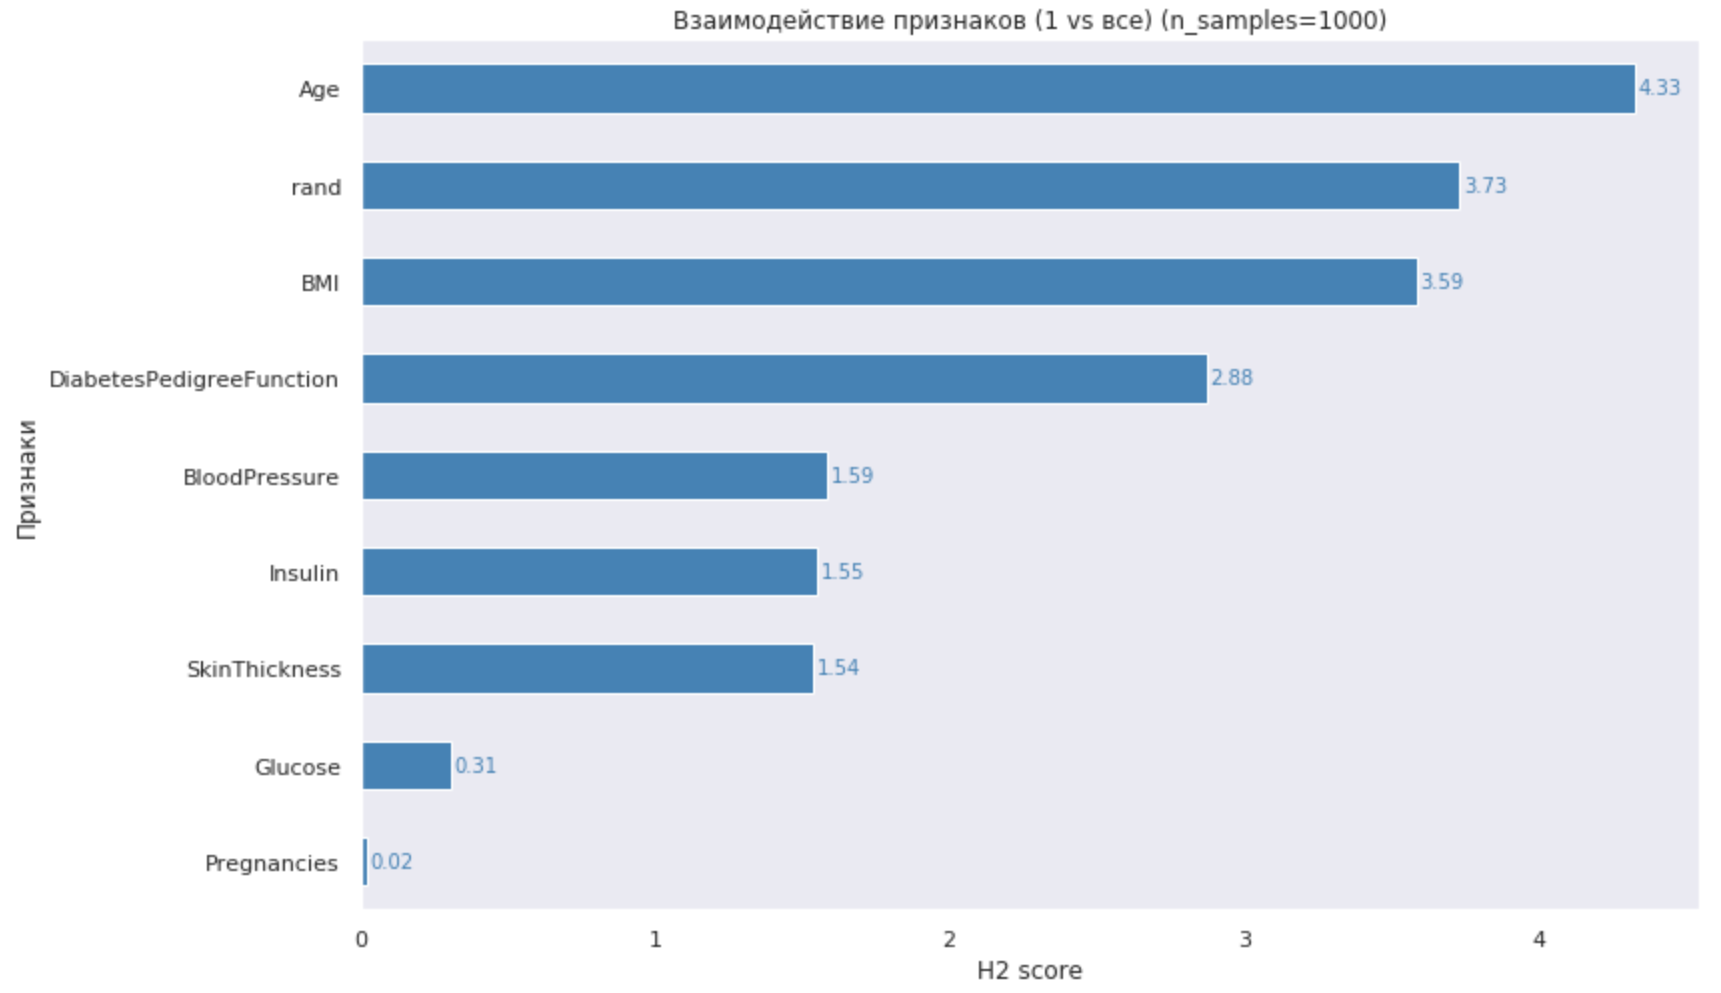
\includegraphics[width=140mm]{images/h2_diab.png}
\end{figure}

Логично увидеть возраст на первом месте.

\begin{figure}[h]
\centering
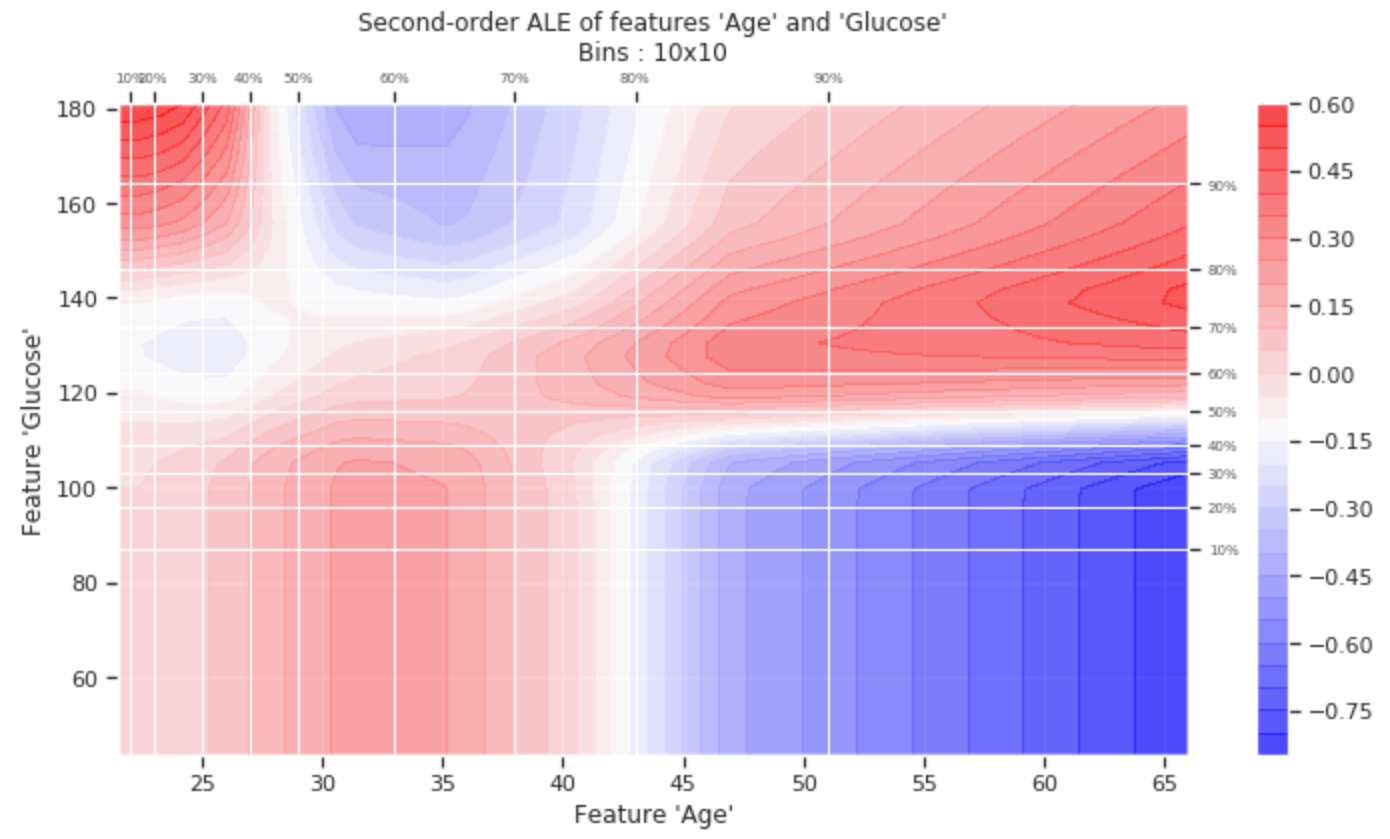
\includegraphics[width=130mm]{images/glucose_diab.png}
\end{figure}


После 44 лет есть четкое пороговое значение по которому можно судить о диабете. При старении становится более важным соблюдать диету, так как небольшие отклонения приводят к резкому повышению вероятности его появления или наоборот.

\newpage
\begin{figure}[h]
\centering
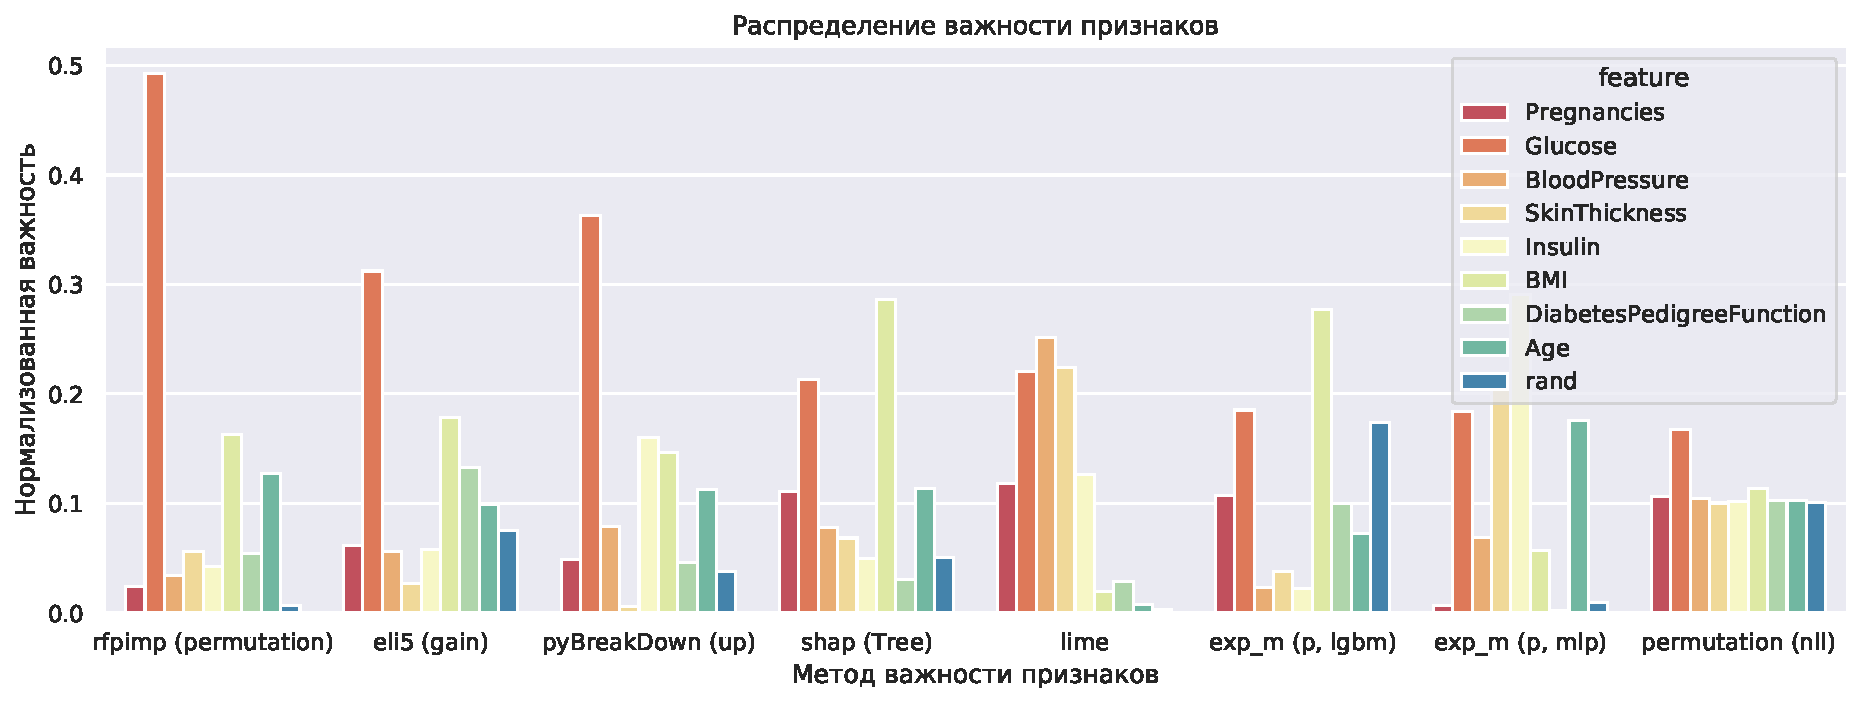
\includegraphics[width=\textwidth]{images/diabets_TargetSum_impFeatures.pdf}
\end{figure}

В большинстве случаев глюкоза и индекс массы тела влияют на наличие диабета. Gain показало высокую важность для случайного признака. Большое число уникальных значений приводит к искусственному увеличению значимости. Permutation (nll) имеет скорее всего неинформативные значения. 

\subsubsection{Удаление признаков}
\begin{figure}[h]
\centering
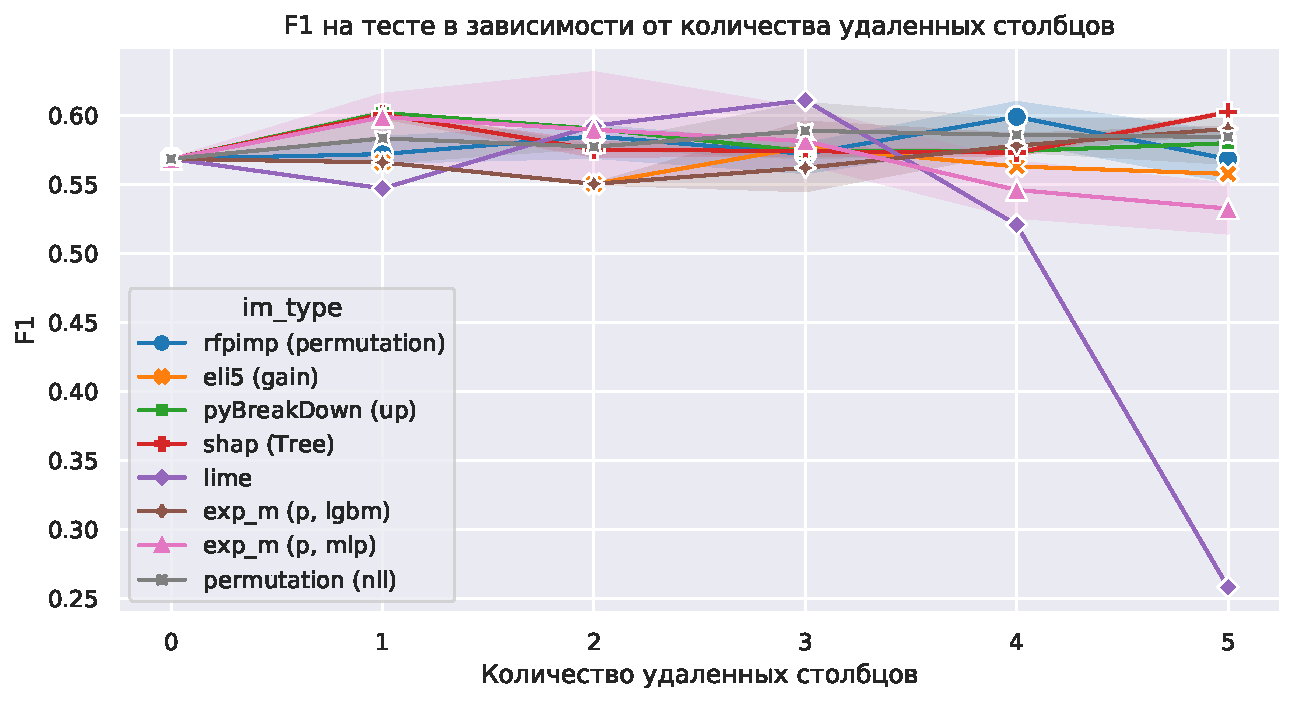
\includegraphics[width=0.7\textwidth]{images/diabets_RFE_f1.pdf}
\end{figure}

На реальных данных все методы, за исключением lime, работают приблизительно одинаково. 

\newpage
\subsubsection{Сэмплирование признаков}
\begin{figure}[h]
\centering
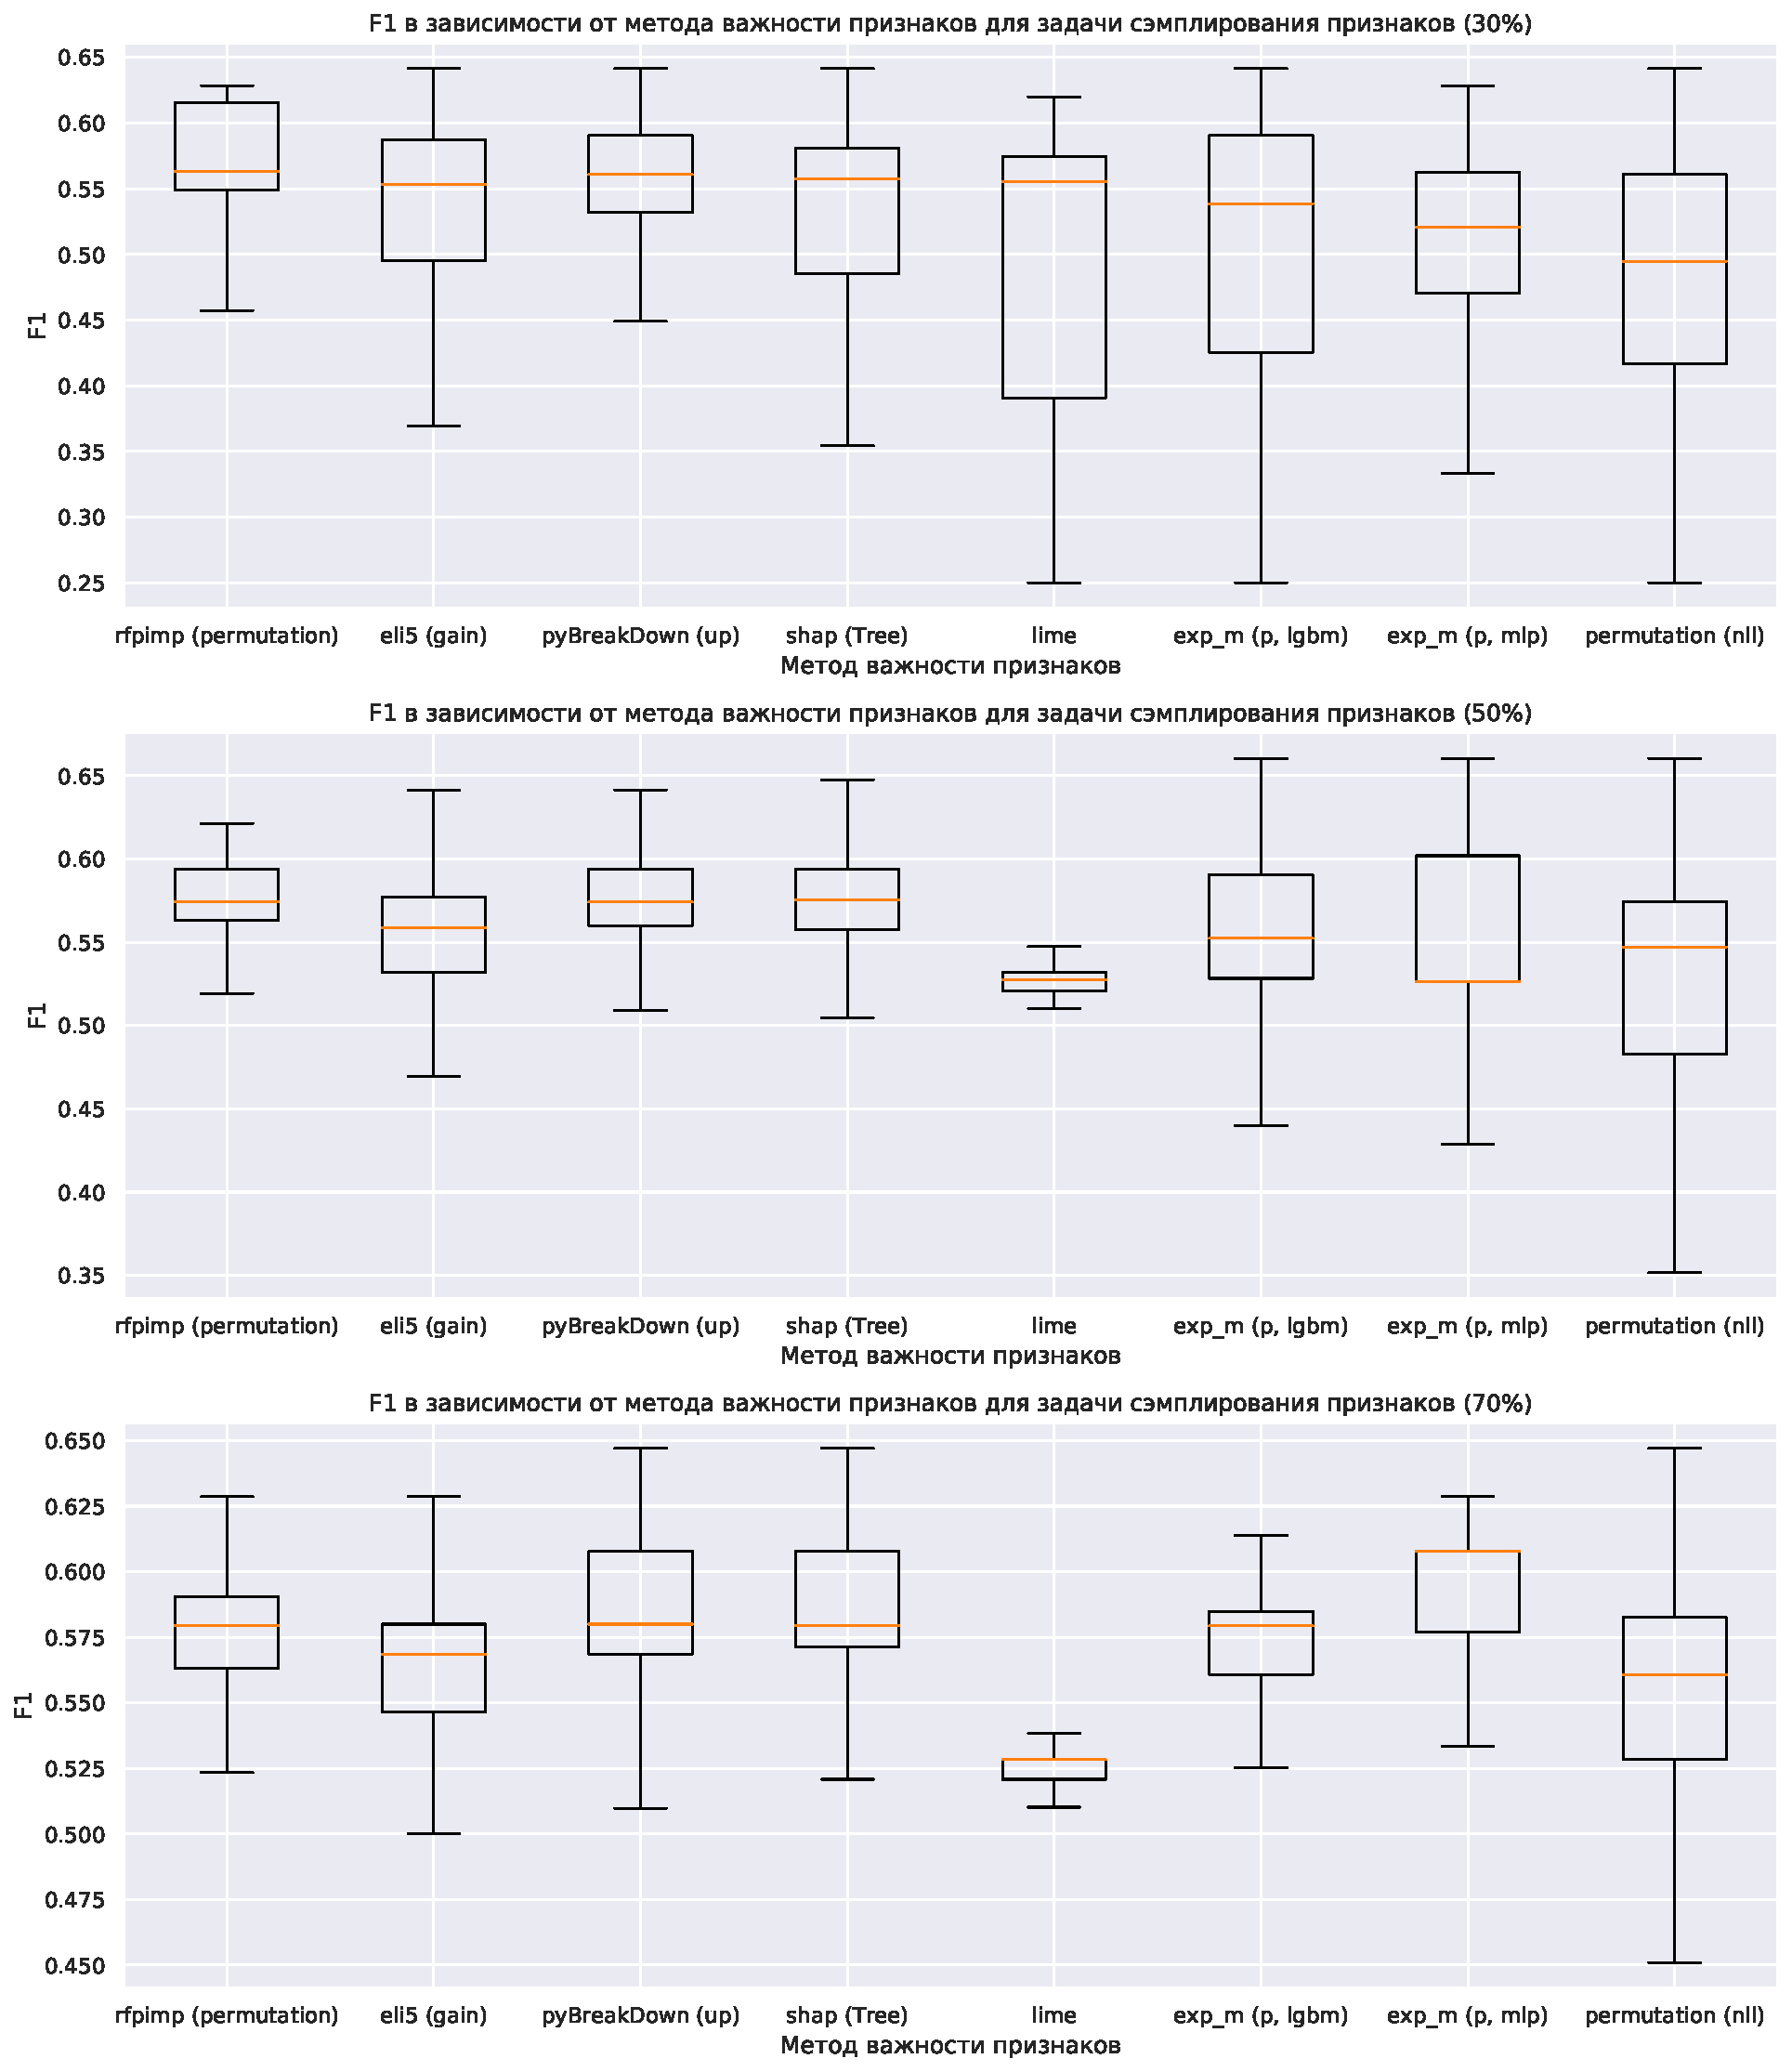
\includegraphics[width=\textwidth]{images/diabets_f1_feature_size.pdf}
\end{figure}

Перестановочная важность лучше всех выделяет признаки, которые в общем нужны для решения задачи (30\% от общего количества). При большом количестве признаков объясняющая модель на основе многослойного перцептрона (MLP) дала лучшие результаты. За исключением lime, признаки, выбранные алгоритмами, дают в среднем одинаковое качество.

\newpage
\section{Заключение}
В данной работе рассмотрены различные методы определения оценки важности признаков. Проведены эксперименты на искусственных и реальных данных, показывающие положительные и отрицательные стороны. Можно сделать следующие выводы:
\begin{itemize}
    \item Прежде чем работать с данными их нужно отфильтровать: кластеризовать похожие признаки и оставить один из них.
    \item Перестановочная важность --- первый метод, который может стать вашим инструментом в поиске важных для задачи признаков, из-за его простоты в применении и относительно небольшой сложности вычисления. Выбор ошибки сильно влияет на его значения.
    \item Если вы интересуетесь нахождением с большой вероятностью важных признаков в малом количестве, то pyBreakDown является хорошим вариантом.
    \item В эксперименте с сэмплированием признаков подход с объясняющей моделью дал лучшие результаты. Однако для релевантных интерпретаций поиск хорошей архитектуры занимает большую часть времени. Для быстроты работы необходима gpu.
    \item Локальные методы, например lime, плохо обобщают информацию на всю выборку данных.
    \item Взаимодействие признака с другими не показало хороший результат, как оценка важности признака.
\end{itemize}


\newpage
\section{Список литературы}
\vspace{-1cm}
% \bibliographystyle{IEEEtran}
\bibliography{F_IM}
\newpage

% \appendix
% \section{Важность признаков}
% \subsection{Дополнение к \ref{art_imortance}}\label{added_art}
% В данном разделе:
% \begin{gather*}
%     y = \mathbb{I}[Z \geq \operatorname{median}(Z)], \hspace{1em}\text{где} \\
%     Z = \operatorname{sigmoid}(\xi_1 gr_{11} + ... + \xi_5 gr_{51})
% \end{gather*}

\end{document}


% Self-supervision --- это обучение без учителя, при котором каким-то образом по имеющимся данным генерируется обучающая выборка $\{x, y\}_i, x \in X, y \in Y$, задающая некоторую \emph{вспомогательную задачу} (auxiliary task) регрессии или классификации, так, что обучаемая на такой выборке \emph{модель} $f: X \to Y$ обладает некоторыми ценными свойствами. Иными словами, задача обучения без учителя сводится к задаче обучения с учителем. Рассмотрим несколько примеров.

% \begin{figure}[h]
% \centering
% \includegraphics[width=140mm]{selfsup_gen}
% \caption{\label{fig:selfsup_gen}Генерация выборки для вспомогательной задачи классификации~\citep{doersch2015unsupervised}.}
% \end{figure}

% \begin{wrapfigure}{L}{0.4\textwidth}
% \centering
% \includegraphics[width=0.35\textwidth]{selfsup_task}
% \caption{\label{fig:selfsup_task}Пример вспомогательной задачи~\citep{doersch2015unsupervised}.}
% \end{wrapfigure}

% \underline{Пример} (Контекстное предобучение на изображениях~\citep{doersch2015unsupervised}). На вход дана коллекция изображений, возможно, разного размера. Требуется научиться распознавать объекты, однако выборки нет. Поскольку состав классов также не задан, целью является обучение представлений изображений, то есть функции $f: \R^{W \times H \times C} \to \R^d$, где $W, H$ --- некоторые заданные высота, ширина изображений, $C$ --- число каналов, $d$ --- размерность обучаемых представлений. Рассматривается ситуация, когда $W, H$ соответствуют относительно небольшой подобласти изображений, и размеры изображений из выборки в несколько раз больше.

% \begin{wrapfigure}{R}{0.24\textwidth}
% \centering
% \includegraphics[width=0.15\textwidth]{selfsup_model}
% \caption{\label{fig:selfsup_model}Сиамская архитектура модели~\citep{doersch2015unsupervised}.}
% \end{wrapfigure}

% Строится вспомогательная задача классификации, для которой обучающая выборка генерируется следующей процедурой: для случайного изображения выбирается случайная подобласть $x_1$ размера $W \times H$. Затем, сэмплируется $y \sim \Uniform\{1, 2, \dots, 8\}$, и в качестве $x_2$ берётся область того же изображения, расположенная в $y$-ой позиции относительно $x_1$ (см.~рис.~\ref{fig:selfsup_gen}). Вспомогательная задача --- по паре $x_1, x_2$ восстанавливать $y$, то есть отвечать на вопрос об относительном расположении двух фрагментов одного изображения (рис.~\ref{fig:selfsup_task}). Такой процедурой генерируется набор прецедентов $\{(x_1, x_2), y\}$ и на нём обучается модель классификации $g(f(x_1), f(x_2))$, где $g$ по конкатенации двух представлений из $\R^d$ выдаёт вероятности восьми классов. Использование сиамской архитектуры (рис.~\ref{fig:selfsup_model}) намеренно: функция $f$ в этой схеме является <<искомой>> и по итогам обучения может использоваться в качестве генератора представлений; совместное обучение $f, g$ требует от функции $f$ выдавать признаки, необходимые для сравнения положения фрагментов. Экспериментально показано, что эти признаки достаточно хорошо описывают содержимое изображений и могут быть использованы для обучения небольшой полносвязной сети (головы) для последующих задач распознавания на предоставленной выборке. \qed

% \vspace{0.2cm}
% \underline{Пример} (BERT~\citep{devlin2018bert}). В области обработки естественного языка BERT стал центральной моделью, демонстрирующей эффективность нейронных сетей на базе архитектуры трансформера~\citep{vaswani2017attention} к задачам на текстах. Предобучение BERT проводится в self-supervised режиме на корпусе неразмеченных текстов. Строятся вспомогательные задачи классификации: входом являются два предложения, разделённые специальным токеном <SEP> и предварённые токеном <CLS>. Несколько слов во входе случайно заменяются специальным токеном <MASK>. Для каждого токена из входной последовательности трансформер выдаёт некоторое представление; модель обучается так, что для токена <CLS> от соответствующего представления требуется кодировать информацию, необходимую для ответа на бинарный вопрос: правда ли, что входные предложения взяты последовательно из одного текста, а для токенов <MASK> соответствующие представления восстанавливают пропущенные слова.

% BERT не столько используется в качестве модели, учащей представления, сколько для transfer learning-а: на заданной выборкой задаче на текстах модель BERT можно дообучать. \qed
% \vspace{0.2cm}

% В этих двух примерах важно, что отсутствие разметки не мешает начинать процесс обучения, выделения интеллектуальных зависимостей в данных. Идея принципиальна тем, что на практике неразмеченных данных можно собрать существенно больше, чем размеченных, и удачно построенные процедуры подобного предобучения могут привести к снижению требований к обучающей выборке (например, необходимого объёма размеченных асессорами данных). Принципиально важно, что переносом знания возможности self-supervised обучения не ограничиваются.

% \vspace{0.2cm}
% \underline{Пример} (Решение задачи трекинга без использования разметки~\citep{vondrick2018tracking}). Даны не размеченные цветные видео. Рассматривается следующая вспомогательная задача: на вход модели подаётся два кадра из одного и того же видео, отстоящие в видеоряде недалеко друг от друга. Первый кадр (референсный) по хронологическому порядку $x^r$ при этом оставлен цветным, а из второго (целевого) $x^t$ информация о цвете удалена. Задачей является восстановление цвета целевого кадра <<аналогично>> референсному кадру.

% \begin{figure}[h]
% \centering
% \includegraphics[width=120mm]{colorization}
% \caption{\label{fig:colorization}Модель для решения задачи раскраски целевого кадра по референсному~\citep{vondrick2018tracking}.}
% \end{figure}

% Модель для решения такой вспомогательной задачи (рис.~\ref{fig:colorization}) представляет собой функцию $f \colon \R^{W \times H} \to \R^{W \times H \times d}$, строящую латентное представление в $\R^d$ для каждого пикселя входного чёрно-белого изображения. Для входа $(x^r, x^t)$ процедура получения выхода модели составляется так: из референсного изображения удаляется цвет, после чего каждое из двух входных чёрно-белых изображений прогоняется через модель $f$ для получения латентных описаний
% всех пикселей. В качестве выходного цвета пикселя $j$ целевого кадра выдаётся взвешенная комбинация цветов референсного кадра $y_j = \sum_{i} w_{i}c_{i}$, где $c_{i}$ --- цвет пикселя $i$ референсного кадра, а веса $w_{i}$ пропорциональны похожести описания раскрашиваемого пикселя на описание пикселей референса:
% $$w_{i} \propto \exp \langle f(x^r)_i, f(x^t)_j \rangle $$

% Выход такого алгоритма дифференцируем по параметрам модели $f$, и, следовательно, возможна стандартная процедура обучения. Эмпирически, по результатам обучения функция $f$ учится выдавать уникальные представления для уникальных объектов: следовательно, если известно, в какой позиции находился некоторый объект на референсном кадре, то, чтобы найти тот же объект на целевом, достаточно найти пиксель с самым похожим описанием из обученной модели $f$. Иными словами, без какого-либо переноса знаний, дообучения и в принципе асессорской разметки, удачная формулировка вспомогательной задачи (и модели для её решения) позволяет решать такую сложную задачу, как задача трекинга. \qed
% \vspace{0.2cm}

% Резюмируя, self-supervised подход постулирует возможность <<интеллектуального>> обучения без разметки на входе, за счёт генерации вспомогательных задач <<самим себе>>. Нас далее будет интересовать применение этой концепции в рамках задачи обучения с подкреплением.

% \subsection{Обучение с подкреплением}

% Задача обучения с подкреплением будет рассматриваться в стандартной постановке~\citep{sutton2018reinforcement}. \emph{Марковским процессом принятия решений} (Markov Decision Process, MDP) называется четвёрка $(\St, \A, \Trans, r)$, где: 
% \begin{itemize}
%     \item $\St \subseteq \R^D$ --- \emph{пространство состояний} (state space).
%     \item $\A$ --- \emph{пространство действий} (action space), либо дискретное ($|\A| < \infty$), либо непрерывное ($\A \subseteq \R^A$).
%     \item $\Trans$ --- \emph{функция переходов} (transition function) или \emph{динамика среды} (world dynamics): формально это вероятности переходов $p(s' \mid s, a)$ и распределение $p(s_0)$ начальных состояний.
%     \item $r: \St \times \A \to \R$ --- \emph{функция награды} (reward function).
% \end{itemize}

% \emph{Распределением траекторий} (trajectory distribution) для заданной \emph{стратегии} или \emph{политики} (policy) $\pi(a \mid s)$ называется распределение
% $$p(\Traj_\pi) \coloneqq p(s_0, a_0, s_1, a_1 \dots ) = p(s_0)\prod_{t=0}^{\infty}\pi(a_t \mid s_t)p(s_{t+1} \mid s_t, a_t).$$

% На каждом шаге $t$ агент получает награду в размере $r_t \coloneqq r(s_t, a_t)$. Задачей обучения с подкреплением является оптимизация средней дисконтированной кумулятивной награды:
% \begin{equation}\label{goal}
% \E_{\Traj_\pi} \sum_{t=0}^{\infty} \gamma^t r_t \to \max_\pi
% \end{equation}
% где $\gamma \le 1$ --- \emph{коэффициент дисконтирования} (discount factor). 

% Для дальнейшего повествования будет важно, что в постановке задачи предполагается:
% \begin{itemize}
%     \item \emph{Марковость} среды: независимость функции переходов и функции наград от истории взаимодействия агента со средой; эти функции зависят только от текущего состояния $s$ и того действия $a$, которое агент в нём выбрал.
%     \item \emph{Стационарность} среды: функция награды и функция переходов не зависят от времени.
% \end{itemize}

% Существуют разнообразные алгоритмы и подходы к решению задачи обучения с подкреплением. В таблице \ref{RLalgorithms} указаны основные характеристики и сокращения названий некоторых из распространённых алгоритмов; используются стандартные обозначения~\citep{sutton2018reinforcement} для оценочной функции состояний $V^\pi$, оценочной функции состояний-действий $Q^\pi$, оптимальной оценочной функции $Q^*$, оптимальной оценочной функции в distributional форме $\mathcal{Z}^*$~\citep{bellemare2017distributional}, детерминированной стратегии $\pi(s)$ и стохастичной стратегии $\pi(a \mid s)$. 

% \vspace{-0.2cm}
% \begin{center}
% \begin{longtable}{| 
% >{\centering}m{2cm}
% >{\centering}m{5cm}
% >{\centering}m{2cm}
% >{\centering}m{2.5cm}
% >{\centering\arraybackslash}m{3cm}
% |}
% \hline
%   \textbf{Сокращение} & \textbf{Алгоритм} & \textbf{Режим} & \textbf{Обучаемые функции} & \textbf{Допустимые пространства действий} \\
% \hline
%   DQN & Deep Q-Network~\citep{mnih2013playing} & off-policy & $Q^*$ & дискретное \\
%   QR-DQN & Quantile Regression DQN~\citep{dabney2018distributional} & off-policy & $\Z^*$ & дискретное \\
%   Rainbow & Rainbow DQN~\citep{hessel2018rainbow} & off-policy & $\Z^*$ & дискретное \\
%   DDPG & Deep Deterministic Policy Gradient~\citep{lillicrap2015continuous} & off-policy & $Q^\pi$, $\pi(s)$ & непрерывное \\
%   A2C & Advantage Actor-Critic~\citep{sutton2000policy} & on-policy & $V^\pi$, $\pi(a \mid s)$ & любое \\
%   PPO & Proximal Policy Optimization~\citep{schulman2017proximal} & on-policy & $V^\pi$, $\pi(a \mid s)$ & любое \\
% \hline
% \caption{\label{RLalgorithms} Основные характеристики некоторых алгоритмов обучения с подкреплением.}
% \end{longtable}
% \end{center}
% \vspace{-1cm}

% Исследование этих алгоритмов ортогонально дальнейшему обсуждению, поэтому детальное описание и теоретические основания этих алгоритмов вынесены отдельно в \href{https://arxiv.org/pdf/1906.10025.pdf}{курсовую работу}~\citep{ivanov2019modern}.

% \subsection{Внутренняя мотивация}

% В обучении с подкреплением типична ситуация \textit{разреженной функции награды} (sparse reward setting), когда агенту редко поступает сигнал от среды. Стандартным примером является использование в качестве функции награды индикатора решения задачи: существует подмножество $\St^* \subseteq \St$, часто совпадающее со множеством терминальных состояний, такое что:
% $$r(s, a) = \begin{cases}
% +1 \quad & s \in \St^* \\
% \const \quad & s \not\in \St^* \\
% \end{cases}$$
% где $\const$ либо равна нулю, либо отрицательному числу, имеющему смысл штрафа за потерю времени. Задача \eqref{goal} задана корректно, однако оптимизируемая функция представляет собой, по существу, плато. Ни один метод оптимизации такую функцию принципиально оптимизировать не может, если только области, где функция не является константой, нельзя как-то <<просто>> найти.

% Если все траектории, которые агент встречает в начале обучения, равноценны, в том смысле, что награда является константой, ни один алгоритм обучения с подкреплением не способен начать обучаться. Проводя аналогию с обучением с учителем, отсутствует разметка: нет никакого сигнала о том, какие действия лучше или хуже (какие ответы более правильные, чем другие). Проблема заключается не столько внутри самих RL-алгоритмов, сколько заложена в постановке самой задачи.

% Возможно ли в такой ситуации начинать какое-либо обучение? Доступным вариантом является постановка self-supervised задач регрессии и классификации на тех траекториях, которые агенту удаётся собрать. Важный пример такой задачи --- обучение аппроксимации функции переходов $p(s' \mid s, a)$; это основной способ, как агент может внутри своей обучающейся системы строить модель мира --- своё представление о том, как работает окружающая его среда. Заметим, что для этого агенту не требуется функция награды.

% Однако даже если рассматривается model-based подход в обучении с подкреплением, когда функция переходов в принципе доступна агенту (или обучается по имеющимся данным) и может использоваться для планирования, вопрос, как эффективно искать пути к состояниям из $\St^*$, остаётся открытым. Скорее всего, если наивное поведение вроде случайного блуждания (использования случайной стратегии) не приводит к неконстантному сигналу, экспоненциальный перебор всевозможных будущих траекторий также не сможет ничего найти за разумное время. При этом, отсутствует какая-либо обратная связь, которая могла бы навести на способы сокращения перебора.

% Self-supervised режим обучения с подкреплением предполагает генерацию агентом сигнала <<самому себе>>. Вспомогательные задачи предлагается ставить не в терминах регрессии или классификации, а в терминах обучения с подкреплением, то есть предъявляя некоторое MDP. Для этого, понятие MDP разделяется на понятие \emph{среды} (environment) и функции награды: то есть, понятие самого процесса принятия решений отделяется от той задачи, мотивацией решить которую и руководствуется агент при выборе действий.

% Под средой далее будем понимать тройку $(\St, \A, \Trans)$. Этого достаточно, чтобы задать некоторый мир, на состояние которого некоторая сущность, называемая агентом, может влиять при помощи своих действий, но недостаточно, чтобы задать в явном виде функционал для оптимизации, то есть недостаточно для постановки строгой математической задачи. Смысл отделения понятия в том, что в одной и той же среде агенту можно ставить разные задачи, и этим разным задачам будет соответствовать своя функция награды. В частности, если агент каким-то образом собирается в self-supervised режиме поставить вспомогательную задачу <<сам себе>>, ему достаточно предъявить только функцию награды.

% Итак, для данного MDP $(\St, \A, \Trans, r^{\extr})$ \textit{вспомогательной self-supervised задачей} называется MDP, заданное четвёркой $(\St, \A, \Trans, r^{\intr})$. Функция $r^{\intr}$, называемая \textit{внутренней функцией награды} (intrinsic reward function) или \textit{виртуальной наградой}, создаётся внутри обучающейся системы при помощи отдельного модуля. Напротив, функция $r^{\extr}$, заданная в самой постановке задачи, называется \textit{внешней функцией награды} (extrinsic reward function). Каждая задача задаёт мотивацию агента: вспомогательная self-supervised задача задаёт \textit{внутреннюю мотивацию} (intrinsic motivation) агента совершать те или иные действия; реальная задача \eqref{goal}, которую агент на самом деле стремится решить, задаёт \textit{внешнюю мотивацию} (extrinsic motivation) агента.

% Введение внутренней мотивации имеет биологическую интерпретацию. Считается, что одним из протекающих в мозге человека процессов является <<генерации награды>>, поощряющая такое поведение, как игра, любопытство, стремление к познанию; оптимизируя такой сигнал, человек способен начинать обучаться, не получая постоянного сигнала от окружающей среды, какие действия нужно или не нужно совершать. В ходе игрового поведения, человек улучшает своё представление о том, как работает мир вокруг него, по каким законам он устроен и как он своими действиями может влиять на будущее состояние мира и вызывать те или иные явления. Такое познание, <<внутренне мотивированное>>, не использующее внешнюю функцию награды, способно стимулировать обучение довольно сложному поведению, навигации в пространстве состояний и открытию неизведанных областей в среде. Подобное более интеллектуальное <<самообучение>> не только ускоряет поиск сигнала от среды, но и позволяет агенту выработать широкий набор умений, которые скорее всего окажутся полезны для достижения заданной внешней наградой цели, какой бы она ни оказалась. 

% \subsection{Совмещение мотиваций}

% С введением внутренней мотивации агент, формально, может решать две различные задачи. Первая задача --- исходная задача:
% $$J^{\extr}(\pi) \coloneqq \E_{\Traj_\pi} \sum_{t=0} \gamma^t r^{\extr}_t \to \max_{\pi}$$

% Вторая задача --- вспомогательная задача, заданная внутренней мотивацией:
% $$J^{\intr}(\pi) \coloneqq \E_{\Traj_\pi} \sum_{t=0} \gamma^t r^{\intr}_t \to \max_{\pi}$$

% На практике же по умолчанию всегда считается, что сам RL-алгоритм оптимизирует сумму мотиваций:
% \begin{equation}\label{sumgoal}
% J(\pi) \coloneqq J^{\extr}(\pi) + J^{\intr}(\pi) \to \max_{\pi}
% \end{equation}

% Это эквивалентно оптимизации кумулятивной дисконтированной суммы внешней и внутренней награды, при которой RL-алгоритм никак не различает сигналы и не использует разложение награды в сумму:
% \begin{equation}\label{motivsum}
% r_t \coloneqq r^{\extr}_t + r^{\intr}_t
% \end{equation}

% Заметим, что режим оптимизации суммы наград в ситуации с разреженной внешней наградой поначалу совпадает с режимом оптимизации только внутренней награды. Пока агент не <<наткнётся>> на источник внешнего сигнала, единственным стимулом обучения будет внутренняя мотивация.

% При этом понятно, что агенту доступно каждое слагаемое по отдельности (внешняя награда выдаётся средой, а внутренняя генерируется внутри самого алгоритма), и это разложение возможно как-либо использовать. В ряде алгоритмов, таких как DDPG, A2C и PPO, обучаются оценочные функции текущей стратегии. Очевидно, что оценочные функции для суммы двух источников наград \eqref{motivsum} представимы\footnote{Понятно, что для оптимальных оценочных функций это представление неверно (сумма максимумов не равна максимуму суммы). Для distributional-формы оценочных функций $\mathcal{Z}^\pi$ разложение верно, но посчитать распределение суммы $\mathcal{Z}^\pi(s, a) \cdfeq \mathcal{Z}^\pi_{\extr}(s, a) + \mathcal{Z}_{\intr}^\pi(s, a)$, зная распределения $\mathcal{Z}^\pi_{\extr}(s, a), \mathcal{Z}_{\intr}^\pi(s, a)$ по отдельности, нельзя в силу наличия в общем случае корреляции между внутренней и внешней наградой.} в виде суммы соответствующей оценочной функции для внутренней мотивации и оценочной функции для внутренней:

% \begin{equation}\label{valuefunctionssum}
% \begin{aligned}
%  Q^\pi(s, a) &= Q^\pi_{\extr}(s, a) + Q^\pi_{\intr}(s, a) \\
% V^\pi(s) &= V^\pi_{\extr}(s) + V^\pi_{\intr}(s)
% \end{aligned}
% \end{equation}

% \begin{wrapfigure}{R}{0.4\textwidth}
% \centering
% \includegraphics[width=0.35\textwidth]{sepheads}
% \caption{\label{fig:sepheads}Архитектура модели для алгоритмов A2C и PPO с разложенной оценочной функцией.}
% \end{wrapfigure}

% Использование разложений \eqref{valuefunctionssum} позволяет внутри алгоритма учить эти оценочные функции по отдельности~\citep{burda2018exploration}, в частности, на практике позволяет по необходимости <<включать>> и <<выключать>> внутреннюю мотивацию во время экспериментов. Для этого в алгоритмах для каждой из двух оценочных функций заводится своя голова в архитектуре модели (рис. \ref{fig:sepheads}).

% Вторым преимуществом разложения является возможность использовать различные коэффициенты дисконтирования $\gamma^{\extr}, \gamma^{\intr}$. Действительно, если дисконтирование разное для разных мотиваций, представление награды \eqref{motivsum} неверно, при том что разложение оценочных функций \eqref{valuefunctionssum} верным остаётся. Использование разных коэффициентов добавляет гибкости в схему, хотя и требует подбирать больше гиперпараметров.

% Ключевым же преимуществом является возможность сделать внутреннюю мотивацию \emph{неэпизодичной} (non-episodic), то есть игнорировать для неё понятие эпизодов. Эпизодичность означает, что если агент знает, что он оказался в терминальном состоянии (а эта информация агенту обычно доступна), то оценочная функция в нём полагается равным нулю (взаимодействие завершилось и никакой награды далее поступать агенту по определению не будет). Неэпизодичность означает, что агент рассматривает весь процесс решения вспомогательной задачи как один большой никогда не заканчивающийся эпизод, игнорируя понятия терминальности состояний. Такой агент учитывает, что если он окажется в терминальном состоянии, то произойдёт \emph{сброс} (reset) среды, и он окажется в стартовом состоянии $s_0 \sim p(s_0)$. Это может мотивировать агента прерывать текущий эпизод ради того, чтобы начать новый. Рассмотрим, когда это может быть полезно, на интуитивном примере.

% \vspace{0.2cm}
% \underline{Пример} (Агент в яме). В среде существует некоторая труднодоступная область, которую агент внутренне мотивирован исследовать (посетить). Агент предпринимает попытку добраться до области, но падает в яму. Оценочная функция для внешней мотивации знает, что из ямы уже не выбраться, и оценивает действие <<закончить эпизод>> как негативное (<<смерть>>), остальные действия как безрезультатные (+0). Оценочной функции для внутренней мотивации также известно, что из ямы уже не выбраться, и, в случае, если она обучается эпизодично, оценивает любые действия как безрезультатные (+0). Если же оценочная функция неэпизодична, агент знает, что он может произвести сброс среды и, в частности, попробовать ещё раз добраться до труднодоступной области. Неэпизодичность может промотивировать агента не сидеть в яме, оттягивая негативный, но неизбежный эффект смерти, а приступить к следующему эпизоду обучения. \qed
% \vspace{0.2cm}

% \subsection{Примеры внутренних мотиваций}

% Внутренняя мотивация не ограничивается задачей исследования среды, о которой речь пойдёт далее. Существуют другие вспомогательные задачи, которые агент может учиться решать в self-supervised режиме:
% \begin{itemize}
%     \item \emph{Empowerment}: рассматривается поиск областей среды, в которых агент в наибольшей степени контролирует происходящее вокруг (<<обладает наибольшей властью>>). В отсутствие сигнала от среды предлагается искать состояния, в которых агенту доступно <<наибольшее количество возможностей>>. Формализации этого понятия проводятся на языке теории информации; например, в простейшей постановке~\citep{klyubin2005all} агент в данном состоянии $s$ должен максимизировать информацию по Шеннону, которую агент может <<передать>> в следующее состояние:
%     $$\int\limits_{\St} \int\limits_{\A} p(s' \mid s, a) \pi(a \mid s) \log_2 \frac{p(s' \mid s, a)}{\int\limits_{\A} p(s' \mid s, a) \pi(a \mid s) da} ds' da \to \max_{\pi(a \mid s)}$$
%     Основным препятствием в такой концепции является масштабирование алгоритмов оптимизации такого функционала с учётом недоступности агенту функции переходов $p(s' \mid s, a)$ в явном виде.
%     \item \emph{Hindsight Experience Replay}~\citep{andrychowicz2017hindsight}: пример совмещения идеи внутренней мотивации с введением формализма мультизадачности. В упрощённом виде, агенту на вход подаётся не только текущее состояние $s$, но и \emph{целевое состояние} (goal state) $g \in \St$. Агент поощряет себя виртуальной +1 в случае достижения целевого состояния, $r^{\intr}(s, g) \coloneqq \mathbb{I}[s = g]$. Во время взаимодействия со средой вместо $g$ агенту может подаваться специальный маркер, означающий поиск состояний из $\St^*$, то есть поиск состояний с сигналом от среды. При этом если агент сгенерировал траекторию, закончившуюся в некотором состоянии $b \not\in \St^*$, агент может модифицировать сгенерированную траекторию и предположить, что достижение состояния $b \in \St$ и было его <<изначальной целью>>. А точнее, в реплей буфер кладётся копия сгенерированной траектории, где во всех посещённых состояниях целевое состояние $g$ заменено с маркера поиска внешнего сигнала на $b$. Для модифицированной сгенерированной траектории верно, что в конце целевое состояние было достигнуто, и агент получил виртуальную +1. Это позволяет начать обучаться отличать такие траектории от примеров, когда целевое состояние достигнуто не было (с генерацией таких примеров проблем не возникает). По сути, агент учится навигации в среде: перемещаться из любого заданного текущего состояния $s$ в заданное целевое состояние $g$.
%     \item \emph{Chaos Minimization}~\citep{berseth2019smirl}: мотивирует агента искать области пространства состояний, где будущее наиболее предсказуемо, <<избегать сюрпризов>>. Интуицией в такой вспомогательной задаче является идея о том, что многие изобретения человечества были созданы для защиты от сюрпризов, которые, зачастую, неприятны. Существуют среды, например, тетрис, где задача <<минимизации хаоса>> коррелирует с задачей самой игры; агент, решающий такую вспомогательную задачу без доступа к внешней функции награды, <<неявно>> решает исходную задачу.
% \end{itemize}

% Заметим, что минимизация хаоса, в некотором смысле, противоположна задаче исследования, где за обнаружение новизны внутренняя мотивация наоборот поощряет агента. Однако задачи не противоречат друг другу: чтобы найти самую <<спокойную>> область среды и научиться до неё добираться, агенту потребуется заняться исследованием окружения и поиском стабильных областей. В этом смысле, задача исследования, вероятно, является наиболее универсальной вспомогательной задачей, которую агент может себе поставить в среде.

% \subsection{Исследование среды}

% В обучении с подкреплением известна \emph{дилемма исследования-использования} (exploration-exploitation dilemma), заключающаяся в том, что если агент на основе имеющегося опыта сделал вывод о том, что некоторое действие предпочтительнее другого, ему необходимо иногда выбирать менее оптимальные согласно текущей оценке действия, чтобы распознать ошибку и скорректировать предпочтения. Примером того, как в теории возникает формальное описание задачи исследования, является теорема о сходимости табличного алгоритма Q-learning~\citep{watkins1992q}, лежащего в основе современных алгоритмов RL. Важным следствием из теоремы является следующее: необходимым условием сходимости является встреча в траекториях всех пар $(s, a) \in \St \times \A$ с ненулевой вероятностью.

% Для решения дилеммы в практических алгоритмах RL встречаются различные эвристики, приведённые в таблице \ref{explorationheuristics}. Все эти эвристики примерно сводятся к тому, что агент иногда принимает решение не совершать жадное (оптимальное по мнению текущих оценок) действие, а выбирает <<заниматься исследованиями>>. Само же исследование сводится (так или иначе) к выбору случайного действия.

% \vspace{-0.2cm}
% \begin{center}
%   \captionsetup{width=.75\linewidth}
% \begin{longtable}{| 
% >{\centering}m{2.5cm}
% >{\centering}m{4cm}
% >{\centering\arraybackslash}m{9cm}
% |}
% \hline
%   \textbf{Алгоритм} & \textbf{Эвристика исследования} & \textbf{Описание} \\
% \hline
% DQN \\ QR-DQN & $\eps$-жадная стратегия & С вероятностью $\eps$ агент выбирает случайное действие \\
% \hline
%   Rainbow & Шумные сети~\citep{fortunato2017noisy} & В веса $Q$-функции добавляется шум с обучаемой дисперсией \\
% \hline
%   DDPG & Шум Орштейна--Ухленбека~\citep{lillicrap2015continuous} & Добавка к действиям скоррелированного между моментами времени шума из процесса Орштейна-Ухленбека \\
% \hline
%   A2C \\ PPO & Энтропийный бонус & В оптимизируемый функционал добавлено поощрение за высокую энтропию стратегии \\
% \hline
% \caption{\label{explorationheuristics} Эвристики для решения дилеммы исследования-использования в практических алгоритмах.}
% \end{longtable}
% \end{center}
% \vspace{-1cm}

% \begin{wrapfigure}{R}{0.4\textwidth}
% \centering
% \includegraphics[width=0.35\textwidth]{exploration}
% \caption{\label{fig:exploration}Иллюстрация сравнения случайного (слева) и более интеллектуального исследования (справа)~\citep{aubret2019survey}.}
% \end{wrapfigure}

% Случайная стратегия является решением задачи исследования, поскольку, формально, с ненулевой вероятностью встретит любую пару $(s, a) \in \St \times \A$ (в предположении, что все состояния в среде достижимы). Однако понятно, что, если представить себе агента в произвольной среде, у которого нет иных целей и задач помимо исследования, случайное поведение не является оптимальным решением. В частности, в случае разреженной функции награды вероятность найти состояния $\St^*$ может быть сколь угодно близка к нулю (хоть и гарантированно отделена от него), и тогда на практике за разумное время обнаружения происходить не будет. Интуитивно, куда более оптимальным поведением является некий интеллектуальный перебор состояний в среде (рис.~\ref{fig:exploration}).

% Для подробного разбора дилеммы существуют исследования, посвящённые упрощённой постановке задачи под названием <<\textit{задача о многоруких бандитах}>> (multi-armed bandits)~\citep{gittins1979bandit}. Дано $A$ игровых автоматов. Для автомата с номером $a \in \{1, 2, \dots A\}$ существует некоторое распределение $p(r \mid a)$, агенту неизвестное. Эпизоды состоят из одного шага: агент выбирает действие $a$, после чего получает награду $r \sim p(r \mid a)$. Задача выбора оптимального действия в такой среде сводится к поиску
% $$a^* \coloneqq \argmax_a \E_{p(r \mid a)} r.$$

% \pagebreak
% На основе имеющегося опыта агент может построить Монте-Карло оценки средней награды для каждого игрового автомата:
% $$Q(a) \approx \frac{1}{n(a)}\sum_{i=1}^{n(a)} r_i \qquad r_i \sim p(r \mid a)$$
% где $n(a)$ --- счётчик выбора действия $a$ за время всего обучения. 

% Эта Монте-Карло оценка является несмещённой оценкой истинного мат.ожидания, но может быть сколько угодно неверной. Одним из способов введения исследований в контексте задачи многоруких бандитов является выбор действия в очередном обучающем эпизоде по следующему правилу:
% $$a = \argmax\limits_a \left[ Q(a) + U(a) \right],$$
% где $U(a)$ можно рассматривать как некоторый бонус за исследование данного действия. Этот бонус разумно выбирать обратно пропорционально частоте выбора действия и пропорционально времени: он мотивирует выбирать действие $a$, если оно редко выбиралось или если прошло достаточно много времени. В частности, в UCB-бандитах~\citep{audibert2010best} формула добавочного слагаемого имеет следующий вид:
% $$U(a) \coloneqq \sqrt{\frac{\log N}{n(a)}},$$
% где $N$ --- счётчик всех обучающих эпизодов. Любопытно, что такое исследование во многом похоже на введение внутренней мотивации: $U(a)$ является условной наградой за исследование действия $a$, и оно тем больше, чем меньше о действии $a$ агенту известно.

% Отсюда можно сделать вывод, что внутренняя мотивация является довольно естественным способом сформулировать задачу исследования. Далее обсуждаются способы, как можно составлять практические алгоритмы генерации для произвольных сред (троек $(\St, \A, \Trans)$) поощрения за <<исследования>> $r^{\intr}$. Для данной среды можно провести оптимизацию (условно произвольным RL-алгоритмом) награды, которую генерирует предложенный модуль внутренней мотивации, и проанализировать полученное поведение агента; хорошая внутренняя мотивация должна, например, стимулировать посещение разнообразного множества состояний и <<игровое поведение>>, нацеленное на взаимодействие с доступными объектами в среде. 

% \newpage
% \section{Исследование как внутренняя мотивация}\label{curiositychapter}

% \subsection{Оракулы}

% Рассмотрим простой интуитивный способ введения \emph{исследовательских бонусов} (exploration bonuses) в случае табличного MDP, когда $|\St| < \infty$, причём количество состояний достаточно небольшое, чтобы возможно было явно хранить функционалы от состояний $\St \to \R$ в памяти. Несмотря на это допущение, всё равно предполагается, что задача решается на основе опыта взаимодействия со средой без использования функции переходов (агент не имеет доступа к $\Trans$), при помощи алгоритмов табличного обучения с подкреплением, таких как Q-learning или SARSA~\citep{sutton2018reinforcement}.

% Первым вариантом является введение \emph{эпизодичной} (episodic) внутренней мотивации в виде поощрения за посещения состояний, в которых агент не был в течение данного обучающего эпизода:
% $$r^{\intr}(s_t) \coloneqq \mathbb{I}[\forall t' < t \colon s_t \neq s_{t'}]$$
% Такое введение можно рассматривать как эвристику: максимальная кумулятивная внутренняя награда соответствует посещению всех состояний в среде. 

% Однако, как явно видно в формуле, такая функция награды игнорирует требование марковости к MDP. В описании состояний в общем случае не хранится информации о ранее посещавшихся состояниях, и MDP, задающее вспомогательную задачу исследования с такой функций награды, вообще говоря, задано некорректно. Формально, введение эпизодичной внутренней мотивации требует рассмотрения более общей постановки задачи обучения с подкреплением, а именно \emph{частично наблюдаемых марковских процессов принятия решений} (PoMDP)~\cite{kaelbling1998planning}.

% Альтернативным вариантом является введение \emph{нестационарной} (non-stationary) внутренней мотивации в виде функции только от текущего состояния, которая, однако, меняется с ходом обучения, и значение которой обратно пропорционально частоте посещения состояния за время всего обучения. А именно, пусть $n(s)$ --- счётчики посещения состояний; подобные счётчики в конечных MDP суть есть ненормированные плотности распределения <<знакомых>>, <<открытых>> состояний. Чем меньше плотность в очередной точке, тем новее очередное состояние, и тем больше внутренняя мотивация за исследования должна агента поощрить:
% $$r^{\intr}(s) \coloneqq \frac{1}{n(s)}$$

% Нарушение требования стационарности в MDP, формально, также некорректно, поскольку на стационарность опирается теория, лежащая в основе многих RL-алгоритмов, в первую очередь, off-policy алгоритмов, использующих реплей буферы. Введение же любой внутренней мотивации при этом предполагает, что вспомогательная задача будет решаться с их помощью.

% У нестационарности внутренней мотивации есть <<оправдание>>. Поскольку генератор внутренней мотивации есть часть обучающейся системы, он также может эволюционировать (обучаться) с течением времени, аналогично самой стратегии агента и прочим вспомогательным функциям внутри RL-алгоритма. В качестве <<обучения>> генератора внутренней мотивации в простейшем случае является хранение и обновление счётчиков посещения состояний, однако в более сложных моделях могут встречаться процессы обучения вспомогательных self-supervised задач регрессии и классификации. По этой причине, в исследованиях внутренней мотивации доминирует использование в качестве базовых RL-алгоритмов on-policy подходов, таких как A2C и PPO.

% Для более сложных пространств состояний возможно сведение к вышеописанным идеям для табличного MDP. Простым обобщением идеи счётчиков на произвольные пространства состояний является построение оценки плотности $p(s)$ на множестве встречавшихся в ходе всего обучения состояний~\citep{bellemare2016unifying, ostrovski2017count, fu2017ex2}. Однако для получения адекватного сигнала необходимо строить модель так, чтобы оценка плотности была достаточно точной; в сложных пространствах состояний, таких как картинки, обучение подобных моделей зачастую дорого, а их оценки недостаточно точны.  

% Доступен другой способ <<свести>> задачу к идеям табличного случая, если возможно придумать разумную хэш-функцию состояний $h \colon \St \to H$, $|H| < \infty$. Тогда, в эпизодичном случае, агент поощряется за посещение состояний с ранее не встречавшимся в течение эпизода хэшем; в нестационарном случае при обучении хранятся счётчики встречавшихся хэшей. Например, если в среде агент находится в некотором двумерном или трёхмерном пространстве и имеет доступ к своим текущим координатам, простейшим примером хэш-функции является разделить пространство на ячейки и выдавать номер ячейки, в которую попало текущее состояние~\citep{savinov2018episodic}.

% Используемые хэш-функций, часто называемые \emph{оракулами} (oracle), являются, вообще говоря, эвристиками, по сути модифицирующими функцию награды с использованием domain knowledge --- специализированных знаний о среде, в которой решается задача. При решении практических задач подобные трюки бывают крайне полезны и могут существенно упростить решение конкретной задачи; однако нас далее будут интересовать более универсальные подходы, не требующие каких-то предположений о среде и которые могут быть применены в произвольных пространствах состояний.

% Заметим, что почти всегда они отталкиваются или тесно связаны с вышеописанными эвристичными идеями для табличных MDP, в первую очередь с нестационарной формой; существуют обобщения и эпизодичного подхода~\citep{savinov2018episodic}, однако в нём агент выучивает поведение, перебирающее все состояния в том числе по результатам обучения. В некоторых ситуациях это может быть полезным эффектом (когда сама задача является задачей поиска с меняющейся от эпизода к эпизоду целевой точкой). Без механизма <<переключения>> на внешнюю мотивацию итоговое поведение агента, вообще говоря, будет неоптимальным с точки зрения исходной задачи. В нестационарном же подходе счётчики посещения всех состояний в пределе будут стремиться к бесконечности, и после условно бесконечного числа эпизодов обучения внутренняя мотивация <<затухнет>>, сойдясь к тождественно нулевой функции; тогда, агент естественным образом переключится на оптимизацию исходной, внешней награды. В дальнейшем будет обсуждаться введение внутренней мотивации в нестационарной форме.

% \subsection{Дистилляция случайной сетки (RND)}

% Рассмотрим альтернативный способ оценки новизны очередного состояния, не требующий явно или неявно оценивать плотность распределения встречавшихся состояний. Для моделей классического машинного обучения справедливо наблюдение, что ошибка модели тем больше, чем менее похож входной объект на объекты обучающей выборки. Отличие предсказания модели от истинного значения целевой переменной может быть использовано как приближение оценки новизны (или \emph{аномальности}) данных (рис. \ref{fig:novelty}).

% \begin{figure}[h]
% \centering
% \includegraphics[width=120mm]{novelty}
% \caption{\label{fig:novelty}Иллюстрация оценки новизны в задаче регрессии.}
% \end{figure}

% Допустим, задана некоторая целевая функция $\phi \colon \St \to \R^d$ --- некоторая детерминированная, стационарная (не меняющаяся с ходом обучения) функция, зависящая только от состояния $s$. Тогда, если модель $f \colon \St \to \R^d$ учится решать вспомогательную задачу регрессии, используя в качестве обучающей выборки $\{ s_i, \phi(s_i) \}_i$, где $s_i$ --- встречавшиеся в ходе обучения состояния, то ошибка модели\footnote{здесь и в аналогичных местах далее в качестве функции потерь для регрессии используется MSE, однако возможно использование любой другой. В частности, в неофициальных реализациях встречаются комбинации, когда оптимизация в модуле внутренней мотивации проходит с использованием одной функции потерь (например, MSE), а сама внутренняя награда рассчитывается, исходя из другой (например, MAE); так может делаться, в частности, из-за более <<удобного>> для базового RL-алгоритма соотношения масштаба внутренней награды между известными и новыми состояниями.} на очередном состоянии $s$ может рассматриваться как обучающий сигнал:
% $$r^{\intr}(s) \coloneqq \|f(s) - \phi(s)\|_2^2$$

% Существенно, что $\phi$ должна быть детерминированной, стационарной и зависеть только от состояний. Действительно, если $\phi$ недетерминирована, ошибка модели для состояния $s$ будет (если, например, $f$ обучается на минимизацию MSE) в среднем равна дисперсии $\phi(s)$. В такой ситуации сигнал внутренней мотивации будет выше в тех областях пространства состояний, где дисперсия $\phi(s)$ выше. Нестационарность, очевидно, нарушает идею подхода, поскольку ошибка модели будет связана с изменением целевой переменной, а не новизной входного состояния. Если же $\phi$ гипотетически построена так, что зависит не только от входного состояния, модель, получающая на вход только $s$, принципиально не сможет выучить целевое значение и будет ошибаться (опять же, возможно, сильнее в одной области пространства состояний по сравнению с другой). Все эти эффекты являются нежелательными, и построение целевой функции $\phi$ следует проводить исходя из соображения избежать этих явлений.

% \begin{wrapfigure}{L}{0.6\textwidth}
% \centering
% \includegraphics[width=0.55\textwidth]{RND}
% \caption{\label{fig:RND}Метод дистилляции случайной сетки (RND).}
% \end{wrapfigure}

% В методе \emph{дистилляции случайной сетки} (Random Network Distillation, RND)~\citep{burda2018exploration} предлагается использовать в качестве $\phi$ случайно инициализированную произвольную нейросеть, принимающую на вход текущее состояние $s$ и выдающую некоторое представление из $\R^d$. Случайная сеть (target network\footnote{название не имеет отношения к эвристике таргет-сети из алгоритмов на основе DQN; однако, как и в DQN, эта случайная сеть здесь используется исключительно для генерации целевых переменных, или <<таргетов>>.}) задаёт детерминированное преобразование только от поданного на вход состояния, а, поскольку веса сети после инициализации в ходе обучения полагаются неизменными, гарантируется стационарность\footnote{внутренняя награда при этом, конечно же, останется нестационарной, так как с ходом обучения изменяется $f$.} $\phi$.

% Соответственно, модель $f$, некоторая другая нейросеть $\St \to \R^d$ (predictor network), обучается предсказывать выходы случайной нейросети (рис. \ref{fig:RND}):
% $$\E_s \|f(s) - \phi(s) \|^2_2 \to \min_f$$
% Здесь мат.ожидание $\E_s$ берётся из распределения посещённых состояний; на практике, в качестве мини-батчей в оптимизатор подаются наборы состояний из батчей переходов, подаваемых на вход RL-алгоритму. Алгоритм назван \emph{дистилляцией}, поскольку одна нейросеть обучается на выходах другой (случайная нейросеть <<дистиллируется>> в модель $f$).

% Авторы подхода продемонстрировали, что сигнал внутренней мотивации, генерируемый таким образом, позволяет обучаться на одной из самых сложных Atari сред <<Месть Монтесумы>>, и впервые смогли достигать конца первого уровня после 500 миллионов итераций обучения, не используя никакой вспомогательной информации о среде. Однако настройка метода сопряжена с рядом нюансов. Во-первых, в сложных средах зачастую верно, что всевозможные состояния похожи как изображения в пространстве исходного представления. Инициализация случайной сетки может пройти так, что $\phi(s)$ будет выдавать примерно константу для всех состояний. В такой ситуации, модели $f(s)$ достаточно легко обобщиться, научившись выдавать константу, чтобы внутренняя мотивация <<затухла>> и быстро сошлась к бесполезному нулевому сигналу. Для борьбы с этим авторы предлагают нормировать состояния, однако статистики нормировки при этом должны быть зафиксированы до начала использования внутренней мотивации внутри RL-алгоритма --- в противном случае изменение статистик приведёт к проблеме нестационарности целевой переменной (для данного входа $s$ при смене нормировочных статистик значение $\phi(s)$ изменится).

% Также авторы предложили нормировать сигнал внутренней мотивации на его бегущее среднее отклонение. Иными словами, предлагается в среднем на каждой итерации выдавать в качестве внутренней награды некоторую константу; это осмысленно с точки зрения обучения, поскольку RL алгоритму принципиальна разница в сигнале, а не его абсолютное значение. Нормировка внутренней мотивации, однако, приведёт к тому, что мотивация исследований не будет затухать, что может быть логично в таких сложных средах, как <<Месть Монтесумы>>, где и после полмиллиарда итераций в среде остаются неисследованные области.  

% \subsection{Любопытство}

% В обучении с подкреплением model-free алгоритмами называются подходы, в рамках которых агент не имеет доступа и при этом никак не пытается учить функцию переходов $p(s' \mid s, a)$. Все алгоритмы, представленные в таблице \ref{RLalgorithms}, относятся к категории model-free. Использование функции переходов или её приближения в алгоритме обычно называют \emph{планированием} (planning), так как сводит задачу к рассмотрению различных вариантов будущего и выбора наилучшего развития событий с учётом прогноза. Интуитивно кажется, что люди во время принятия решений занимаются планированием и строят какие-то предположения о предстоящем будущем, то есть выходят за рамки model-free подхода.

% В предположении марковости, стационарности и полной наблюдаемости, в формализме MDP агенту достаточно выучить функцию переходов $p(s \mid s, a)$ и функцию внешней награды $r^{\extr}(s, a)$ (если она недоступна агенту в явном виде), чтобы полностью <<узнать>> законы окружающего мира. Получение этих функций не означает решение задачи обучения с подкреплением, то есть задачи оптимизации \eqref{goal}: даже если бы эти функции были бы известны агенту, что рассматривается в исследованиях model-based подхода в обучении с подкреплением, поиск комбинаций действий, которые приведут к траектории с максимальной выгодой, является экспоненциальным.

% \emph{Любопытством} (curiosity)~\citep{schmidhuber1991curious} по определению называется ошибка модели мира. Ошибка свидетельствует о том, что агент не всё знает о той области пространства состояний, в которой был произведён неверный прогноз. Использование любопытства как внутренней мотивации приводит к тому, что агент стремится в те области среды, которые ему <<непонятны>>, в частности те, которые для агента новы.

% Такая концепция любопытства представляет собой альтернативную парадигму введения внутренней мотивации исследований. Она отличается от концепции, где сигнал мотивации пропорционален новизне состояний, что можно увидеть в следующем мысленном эксперименте:

% \vspace{0.2cm}
% \underline{Пример} (Бесконечные двери). В ряд стоит бесконечное количество одинаковых дверей, за каждой из которых ничего нет. Агенту доступен на вход, помимо прочего, номер двери. Сигнал, построенный на основе оценки новизны состояний, будет поощрять обнаружение новых дверей, поскольку их номер нов по сравнению со старыми. Любопытство же через некоторое время научится предсказывать, что при движении вдоль ряда агенту будут встречаться точно такие же двери, как и раньше, и что за дверьми ничего нет; сигнал затухнет. При этом, любопытство среагирует на любое изменение в описании двери, или если за очередной дверью окажется что-то непредсказуемое. \qed
% \vspace{0.2cm}

% Эта разница достаточно условна: предполагается, что модель предсказания будущего способна <<обобщаться>> на новые состояния, что, в целом, может оказаться верным и для модели оценки новизны. Так, в приведённом примере модель оценки новизны также может перестать оценивать увеличение номера двери как <<новые>> состояния, и тогда поведение модулей внутренней мотивации станет схожим.

% Далее предполагается, что итоговый алгоритм остаётся условно model-free в том смысле, что, хоть в системе и будет обучаться явно или неявно приближение функции переходов, оно не будет использоваться при самом принятии решений для приближённого планирования, а будет использоваться исключительно в модуле для генерации внутренней мотивации в качестве модели мира; учить функцию внешней награды при этом не потребуется. Совмещение model-based подходов с модулями генерации любопытства остаётся открытым вопросом для исследований.

% \subsection{Модель прямой динамики}

% Итак, в простейшем случае для моделирования любопытства достаточно обучать детерминированную функцию, называемую \emph{моделью прямой динамики} (forward dynamics model) $f \colon \St \times \A \to \St$. Проводить обучение возможно в self-supervised режиме, используя  в качестве обучающей выборки произвольные доступные агенту траектории (в том числе, возможно, из реплей буфера):
% $$\E_{s,a,s'} \|f(s, a) - s'\|^2_2 \to \min_f$$
% Здесь мат.ожидание берётся по $s, a, s'$, таким что $s' \sim p(s' \mid s, a)$; иных требований к распределению, откуда берутся тройки, предъявлять нет необходимости. Это означает, что тройки могут как браться из реплей буфера для off-policy алгоритмов, так и браться из текущих мини-батчей для основного RL-алгоритма в on-policy подходах. Достаточно предполагать, что тройки берутся из опыта агента, то есть соответствуют посещённым областям среды.

% Во время очередного обучающего эпизода ошибка модели на каждом шаге является любопытством и задаёт внутреннюю мотивацию агента:
% \begin{equation}\label{curiosity}
% r^{\intr}(s, a, s') \coloneqq \|f(s, a) - s'\|^2_2
% \end{equation}

% Для пространства состояний, заданного изображениями, модель $f$ может быть построена стандартным образом (рис. \ref{fig:forwardmodel}). Свёрточная сеть-кодировщик преобразует входное изображение $s$ в компактное представление, конкатенирует с описанием входного действия $a$ (если пространство действий дискретно, то оно задаётся one-hot кодированием), после чего полученный вектор отправляется в декодировщик, состоящий из transposed-свёрток, и генерирующий на выходе приближение $s'$.

% \begin{figure}[h]
% \centering
% \includegraphics[width=120mm]{forwardmodel}
% \caption{\label{fig:forwardmodel}Архитектура модели прямой динамики.}
% \end{figure}

% Подход обладает рядом существенных принципиальных недостатков. В сложных пространствах состояний их описание обычно содержит огромное количество никак не связанной с задачами агента информацией (например, декоративные элементы в видеоиграх). Построение и обучение подобного декодировщика сопряжено с бессмысленным изучением этой информации. Наконец, в формуле \eqref{curiosity} сгенерированное изображение сравнивается с полученным в траектории исходом по l2-метрике, что для изображений бессодержательно; такой сигнал скорее всего будет мотивировать агента искать сложно предсказуемые декоративные элементы в среде, которые декодировщику сложнее выучить, при том он будет слабо реагировать на появление важной информации на небольшом числе сенсоров. Основной же проблемой модели является то, что функция переходов принципиально стохастична, и приближение её детерминированной моделью в большинстве ситуаций неоправданно.

% Несмотря на эти недостатки, для простейших сред модель прямой динамики в таком виде может полноценно использоваться для моделирования любопытства; негативные эффекты полностью проявляются в сложных пространствах состояний вроде изображений. Если состояния заданы компактным вектором $\St \subseteq \R^D$ и вся информация в них является ценной, l2-метрика может являться вполне осмысленной. Единственным недостатком подхода тогда остаётся только детерминированность модели --- даже в простых средах это сопряжено с основной фундаментальной проблемой концепции любопытства, называемой проблемой <<шумного телевизора>>.

% \subsection{Проблема <<шумного телевизора>>}

% Аналогично дистилляции случайной сетки, использование ошибки некоторой модели в качестве мотивации может привести к нежелательным эффектам, если целевая переменная недетерминирована, нестационарна или задана слишком сложной зависимостью для используемого параметрического семейства. Для модели прямой динамики целевая переменная стационарна в рамках предположения о стационарности функции переходов $\Trans$ в MDP, однако она (в общем случае) недетерминирована. Это означает, что агент будет стремиться к тем областям среды, где в функции переходов присутствует больше стохастики, и где модель предсказывает не следующее состояние, а, например, усреднённое следующее состояние по всевозможным исходам.

% \vspace{0.2cm}
% \underline{Пример} (Шумный телевизор). В среде присутствует сломавшийся телевизор, демонстрирующий гауссовский шум. На каждом шаге шум независимо сэмплируется заново. Предсказывать следующее значение шума по предыдущему в силу независимости сэмплов невозможно. В рамках концепции любопытства, агент мотивирован найти подобный <<шумный телевизор>> в среде и получать наслаждение от непредсказуемости своих будущих наблюдений. \qed
% \vspace{0.2cm}

% <<Шумные телевизоры>> могут принимать самые разные формы. Во-первых, это могут быть любые принципиально непредсказуемые явления в среде, когда исход $s'$ зависит от случайности $z$, не заложенной в заданном состоянии-действии $p(z) = p(z \mid s, a)$:
% $$p(s' \mid s, a) = \int\limits_z p(s' \mid s, a, z)p(z)dz$$
% При этом вид шума $z$ может быть произволен: это может быть гауссовский шум на, например, сломанных сенсорах агента (рис. \ref{fig:noisyinput}); бинарная латентная переменная, соответствующая броску монетки в игре; источник шума для генератора случайных текстур на стенах лабиринта или иных декоративных элементов; номер случайного изображения из коллекции для демонстрации на экране телевизора в среде.

% \begin{wrapfigure}{R}{0.3\textwidth}
% \centering
% \includegraphics[width=0.25\textwidth]{noisyinput}
% \caption{\label{fig:noisyinput}Пример входа со <<сломанными сенсорами>>.~\citep{pathak2017curiosity}}
% \end{wrapfigure}

% Основное свойство шумных телевизоров --- нерелевантность для агента. В большинстве, но не во всех, примерах подобная стохастика не имеет отношения к самой задаче агента: сломавшиеся сенсоры и декоративные текстуры не содержат никакой полезной информации (рис.~\ref{fig:towerobstacle}). Если бы для большинства сред шумные телевизоры не обладали этим свойством, разумным подходом было бы обучение недетерминированной модели функции переходов, то есть построение генеративной модели $q(s' \mid s, a)$; в ситуациях, когда стохастика среды существенно влияет на будущее агента и его путь к целевым состояниям, знание и понимание вероятностей различных исходов и их состав, очевидно, является ценным знанием об окружающем мире. Однако даже если в среде нет нерелевантного шума, остаётся открытым вопрос о построении значения любопытства: агент во время обучающего эпизода имеет доступ лишь к тройке $s, a, s'$, и необходимо для данного перехода без прямого доступа к $p(s' \mid s, a)$ получать значение или хотя бы несмещённую оценку (в формализме MDP допускается стохастичная функция награды) ошибки $\mathcal{D}(p(s' \mid s, a) \parallel q(s' \mid s, a))$, где $\mathcal{D}$ --- некоторая метрика в пространстве вероятностных распределений в $\St$. Даже если подобный практический алгоритм удастся построить, шумные телевизоры скорее всего задаются сложным распределением, которое в принципе будет плохо поддаваться изучению. В совокупностью с нерелевантностью шумных телевизоров, решения подобной задачи хотелось бы принципиально избежать.

% \begin{wrapfigure}{L}{0.3\textwidth}
% \centering
% \includegraphics[width=0.25\textwidth]{towerobstacle}
% \caption{\label{fig:towerobstacle}Пример шумных телевизоров в среде Unity Obstacle Tower.~\citep{juliani2019obstacle}}
% \end{wrapfigure}

% Вторым не менее важным примером шумных телевизоров являются ситуации, когда функция переходов просто настолько комплексна, что агенту понадобится обучать дорогую и сложную модель. Даже если среда детерминирована, агент будет получать огромную мотивацию возвращаться в область с подобным шумным телевизором до тех пор, пока сложная модель не будет обучена. Если же обучение не удастся в силу простоты обучаемой модели или неидеальности процесса оптимизации, агент <<застрянет>> в области и никогда не переключится на исследование остального окружения. Примеры таких шумных телевизоров проще привести из реальной жизни: человек не пытается моделировать все без исключения окружающие сложные процессы, например, предсказывать поведение (траектории) всех наблюдаемых капель дождя или опадающих листьев. Как и в предыдущем случае, подобная информация редко связана с непосредственными задачами агента в средах, и тратить ресурсы (итерации обучения) на детальное восстановление функции переходов бессмысленно.

% В ранних работах по введению любопытства в формализм обучения на основе опыта предлагалась интуиция решения проблемы~\citep{schmidhuber2010formal}: сигналом внутренней мотивации должна быть не столько ошибка модели, сколько её изменение после дообучения. Иными словами, если модель продолжает ошибаться, <<понимать явление>> в среде не удаётся, необходимо почувствовать разочарование (убрать мотивационный сигнал) и бросить силы на исследование других областей среды. Существуют формализации этой идеи, например, на байесовском языке, когда модель прямой динамики является байесовской нейросетью, и оптимизируется расстояние по некоторой метрике между апостериорным распределением до и после получения очередного состояния~\citep{houthooft2016curiosity}. Ещё одной переформулировкой определения любопытства является использование ансамбля моделей мира и введение мотивирующего сигнала как несогласованности между их прогнозами~\citep{pathak2019self}.

% \subsection{Латентные пространства для модели прямой динамики}

% Распространённым способом борьбы с недостатками любопытства на основе модели прямой динамики является переход к иному представлению состояний, в котором данные о шумных телевизорах будут отфильтрованы~\citep{burda2018large}.

% Допустим, имеется некоторая функция $\phi \colon \St \to \R^d$, далее называемая \emph{фильтром}. В пространстве представлений состояний, полученных при помощи этой функции, строится модель прямой динамики, а то есть по представлению состояния и действию предсказывается представление следующего состояния:
% $$\E_{s,a,s'} \|f(\phi(s), a) - \phi(s')\|^2_2 \to \min_f$$

% Из каких соображений необходимо искать фильтр? Во-первых, представление должно быть компактным, чтобы использование l2-метрики для сравнения предсказаний с исходом было наиболее осмысленным. Во-вторых, предпочтительнее стационарные (стабильные) фильтры, которые меняются или редко меняются в течение процесса обучения; если фильтр $\phi$ изменяется, меняется задача регрессии, которую решает модель прямой динамики, и в момент смены задачи в сигнале на основе ошибки модели появится скачок, не связанный с новизной.

% Рассмотрим несколько базовых вариантов. Построение модели прямой динамики в исходном пространстве соответствует функции $\phi(s) = s$, которая стабильна, но некомпактна и не фильтрует лишнюю информацию. Вторым вариантом является использование в качестве $\phi$ случайного преобразования аналогично дистилляции случайной нейросети; представление из такого фильтра является компактным и стабильным. Ещё одним преимуществом случайного фильтра является то, что для него не нужно строить модель-декодировщик компактного представления в сложное пространство состояний $\St$. Однако выход случайной сети будет меняться при любом изменении входа $s \in \St$; то есть, например, если в сенсорах присутствует гауссовский шум, выход случайной сети скорее всего останется непредсказуем. 

% \begin{figure}[h]
% \centering
% \includegraphics[width=120mm]{vaeforward}
% \caption{\label{fig:vaeforward}Использование VAE для построения фильтра для модели прямой динамики.}
% \end{figure}

% Возможно также использование в качестве $\phi$ кодирующей части какого-либо автокодировщика, который при сжатии $s \in \St$ в компактное представление будет вынужден удалить <<несжимаемую>> информацию, скорее всего соответствующую шумным телевизорам. Показано, что хорошим вариантом является использование с этой целью \emph{варационного автокодировщика} (Variational AutoEncoder, VAE)~\citep{kingma2013auto}. Вариационный автокодировщик состоит из двух частей: кодировщика $q(z \mid s, \psi) = \mathcal{N}(\mu_\psi(s), \sigma_\psi(s)^2I_{d \times d})$ и декодировщика $p(s \mid z, \psi)$, где $\psi$ --- параметры модели, $z \in \R^d$ --- латентное представление. В ходе обучения агента, VAE тренируется на множестве встречавшихся состояний и строит для них генеративную модель в форме $p_\psi(s) = p_\psi(s \mid z)p(z)$, где $p(z) = \mathcal{N}(0, I_{d \times d})$. 

% В качестве фильтра используется среднее распределения латентной переменной для данного состояния, то есть $\phi(s) \coloneqq \mu_\psi(s)$ (полная схема представлена на рис.~\ref{fig:vaeforward}). Такое представление компактно, но нестабильно, поскольку вариационный автокодировщик придётся дообучать на новых открываемых состояниях (распределение посещаемых состояний изменяется с ходом обучения); оно потенциально фильтрует, например, гауссовский шум, генерация которого в модели ложится на сэмплирование из вариационного распределения $q(z \mid s, \phi)$. Однако вариационный автокодировщик не пытается выделять только релевантную для агента информацию: если шумный телевизор представлен в среде не в виде шума на сенсорах, а в виде трудно предсказуемого контента (что является более типичной ситуацией), информация о нём частично или полностью будет содержаться в $\mu_\psi(s)$.

% \subsection{Модель обратной динамики}

% \emph{Моделью обратной динамики} (inverse dynamics model) называется модель, по состоянию $s$ и следующему состоянию $s' \sim p(s' \mid s, a)$ предсказывающая действие $a$, которое привело к данному переходу. Такая модель тоже представляет собой пример модели мира. Агент, делая шаг в среде, может проверить, а правда ли он может по текущему состоянию $s'$ и предыдущему состоянию $s$ восстановить только что выбранное им действие. Отрицательный ответ может соответствовать ситуации, когда агент открыл новые явления в среде, попал в новую область пространства состояний. В таком случае, ошибка модели обратной динамики может быть использована в качестве любопытства; в частности, в некоторых средах выбор действий, максимизирующих ошибку модели обратной динамики приводила к \emph{возникновению игрового поведения} (emergence of playing behavior), когда агент <<играет>> с доступными для взаимодействия предметами в среде с целью <<сломать>> свою модель обратной динамики~\citep{haber2018learning}.

% Преимуществом модели обратной динамики является то, что построение модели $\St \times \St \to \A$ сопоставимо по сложности с моделями, использующимися внутри основного RL-алгоритма: не требуется построение моделей, выдающих объекты из $\St$.

% Для модели обратной динамики проблема <<шумных телевизоров>> в среде заменяется симметричной проблемой в пространстве действий $\A$. Во многих средах пространство действий для некоторых областей $\St$ может содержать принципиально неразличимые действия. Из формализма MDP по формуле Байеса следует:

% \begin{equation}\label{bayesdynamics}
% p(a \mid s, s') = \frac{p(s' \mid s, a)\pi(a \mid s)}{\int\limits_\A p(s' \mid s, a)\pi(a \mid s) da}
% \end{equation}

% Из формулы видно, что искомое распределение, вообще говоря, существенно зависит от используемой для порождения выборки стратегии $\pi$. Если во всей выборке для обучения модели прямой динамики использовалась стратегия $\forall s \colon \pi(s) \coloneqq \tilde{a}$, то искомое $p(a \mid s, s') = \mathbb{I}[a = \tilde{a}]$ не зависит от входа $s, s'$. В более сложных случаях, когда для обучения используются тройки $s, a, s'$, где $a$ выбирается произвольно (из случайной стратегии или из разнообразного набора стратегий), поиск такого распределения более содержателен, и из формулы видна его тесная связь с функцией переходов $p(s' \mid s, a)$. 

% Однако использование ошибки детерминированной модели $g \colon \St \times \St \to \A$ в качестве обучающего сигнала приведёт к тому, что агента будут привлекать траектории с действиями, энтропия распределения \eqref{bayesdynamics} для которых максимальна. В ряде весьма распространённых (особенно в сложных средах) ситуаций подобная оптимизация будет иметь обычно нежелательные побочные эффекты. Например, если два действия в принципе эквивалентны в некоторой области $\tilde{\St} \subseteq \St$ пространства состояний, то есть $\forall s \in \tilde{\St}, s' \in \St \colon p(s' \mid s, a_1) = p(s' \mid s, a_2)$, то агент будет мотивирован, находясь в $\tilde{\St}$, совершать действия $a_1, a_2$.

% \subsection{Внутренний Модуль Любопытства (ICM)}

% Центральной моделью любопытства является схема \emph{внутреннего модуля любопытства} (Intrinsic Curiosity Module, ICM), основанная на комбинации преимуществ моделей прямой и обратной динамики~\citep{pathak2017curiosity}.

% \begin{wrapfigure}{L}{0.6\textwidth}
% \centering
% \includegraphics[width=0.55\textwidth]{inversemodel}
% \caption{\label{fig:inversemodel}Архитектура модели обратной динамики для дискретного пространства действий.}
% \end{wrapfigure}

% В ICM модель обратной динамики $g \colon \R^d \times \R^d \to \A$ строится в пространстве представлений из фильтра $\phi \colon \St \to \R^d$ и обучается совместно с ним (рис. \ref{fig:inversemodel}). Для непрерывных пространств действий задача выглядит следующим образом:
% $$\E_{s, a, s'} \|g(\phi(s), \phi(s')) - a\|^2_2 \to \min_{g, \phi}$$

% Обучающийся так фильтр $\phi$ выдаёт компактные, но нестабильные представления состояний, поскольку модель обратной динамики должна дообучаться на новых встречающихся тройках $s, a, s'$. Однако главное свойство получаемого таким образом преобразования $\phi$ --- фильтрация информации. Действительно, в промежуточных слоях архитектуры останутся данные только с тех сенсоров, которые могут помочь в определении совершённого действия. Если с некоторым объектом в среде, например, шумным телевизором, нельзя провзаимодействовать, информация о нём не требуется модели для предсказания действия и будет отфильтрована. В частности, такой фильтр научится игнорировать шум в сенсорах. И наоборот, если данные с некоторых сенсоров указывают на совершение определённого действия агента, они останутся в представлении $\phi(s)$.

% \begin{wrapfigure}[18]{R}{0.6\textwidth}
% \centering
% \includegraphics[width=0.55\textwidth]{ICM}
% \caption{\label{fig:ICM}Схема внутреннего модуля любопытства (ICM).}
% \end{wrapfigure}

% Итого, основная идея ICM заключается в использовании преобразования $\phi$ в качестве фильтра для модели прямой динамики:
% $$\E_{s, a, s'} \|f(\phi(s), a) - \phi(s')\|^2_2 \to \min_{f}$$

% Любопытством полагается ошибка только модели прямой динамики; задача обратной динамики решается исключительно для получения хорошего фильтра $\phi$:
% $$r^{\intr}(s, a, s') \coloneqq \|f(\phi(s), a) - \phi(s')\|^2_2$$

% Обе вспомогательные задачи можно решать по произвольным тройкам $s, a, s'$, поэтому в качестве мини-батчей для оптимизации можно использовать те же наборы переходов, что и для основного алгоритма. В частности, поскольку исследования любопытства проводятся на on-policy алгоритмах, в распространённых схемах для обучения модуля реплей буфер не используется, хотя такая возможность есть: обучение моделей мира никак не завязано на текущую стратегию взаимодействия со средой.

% Авторы ICM предложили данные задачи оптимизации совместить, а именно (для непрерывных пространств действий) оптимизировать всю схему end-to-end (рис. \ref{fig:ICM}):
% $$\E_{s, a, s'} \left[ \|g(\phi(s), \phi(s')) - a\|^2_2 + \alpha \|f(\phi(s), a) - \phi(s')\|^2_2 \right] \to \min_{f, g, \phi}$$
% где $\alpha$ --- масштабирующий скалярный гиперпараметр. В этой задаче оптимизации градиенты нигде не останавливаются: в частности, от фильтра $\phi$ требуется построение таких представлений, в рамках которых модели прямой динамики $f$ <<проще всего>> предсказывать будущее. Понятно, что, если бы первого слагаемого (задачи обратной динамики) в таком функционале не было бы, оптимальным решением было бы $\phi(s) = \const$. В таком виде, модель прямой динамики выступает регуляризатором для модели обратной динамики: представления $\phi(s)$ одновременно должны содержать достаточно информации для предсказания выбранных действий и при этом быть максимально простыми.

% Аналогичную схему легко построить для случая дискретных пространств действий, заменив функцию потерь регрессии на функцию потерь классификации для модели обратной динамики:
% $$\E_{s, a, s'} \left[-\log g(a \mid \phi(s), \phi(s')) + \alpha \|f(\phi(s), a) - \phi(s')\|^2_2 \right] \to \min_{f, g, \phi}$$

% \subsection{Прокрастинация}

% Решает ли ICM проблему шумных телевизоров? Теоретически, можно рассчитывать на то, что модель обратной динамики отфильтрует те шумные телевизоры, с которыми агент не может провзаимодействовать. Последнее, однако, может быть неверно, и можно построить специальные среды для демонстрации подобных примеров.

% \begin{example}[Управляемый шумный телевизор]
% В среде присутствует телевизор, демонстрирующий изображение (возможно, осмысленное!) из разнообразного бесконечного набора. У агента есть пульт от телевизора, то есть действие $\hat{a}$, при выборе которого изображение на телевизоре сменяется на случайное из набора. По факту смены изображения между $s$ в $s'$ модель обратной динамики может сделать однозначный выбор о том, что между состояниями было выбрано именно действие $\hat{a}$, следовательно в представлении $\phi(s)$ останется информация о содержимом телевизора. При этом, в силу случайности выбора изображения из набора, предсказать контент телевизора по предыдущему изображению и факту нажатия на пульт невозможно. Следовательно, модель прямой динамики в ICM будет ошибаться на тройках, содержащих $\hat{a}$, и агент будет мотивирован бесконечно выбирать действие $\hat{a}$.
% \end{example}

% \begin{wrapfigure}{L}{0.25\textwidth}
% \centering
% \includegraphics[width=0.2\textwidth]{remotecontrol}
% \caption{\label{fig:remotecontrol}Пример управляемого шумного телевизора: у агента есть пульт, рисующий случайные <<круги>> на стенах лабиринта, никак не связанные с задачей.~\citep{savinov2018episodic}}
% \end{wrapfigure}

% Шумные телевизоры, с которыми агент может провзаимодействовать, представляют собой любые стохастичные явления в среде, которые агент может <<запускать>> своими действиями (рис. \ref{fig:remotecontrol}). Проблему любопытства, связанную с отвлечением агента на подобные управляемые источники случайного контента, называют \emph{проблемой прокрастинации} (procrastination issue).

% Важно отметить, что проблема прокрастинации является не столько проблемой самого алгоритма ICM, сколько концептуальной проблемой любопытства. Наличие у агента возможности взаимодействовать с шумным телевизором потенциально означает, что некоторая комбинация действий приводит к решению искомой задачи в среде (высокой внешней награде), а сам шумный телевизор --- связан с задачей (в примере с управляемым шумным телевизором задача гипотетически могла заключаться в поиске определённого изображения из набора, или совершении определённой комбинации действий при определённых условиях на текущее отображаемое изображение). При этом любопытство, как и любая внутренняя мотивация, вводится из соображений, что априорных знаний об истинной задаче агента не дано, и произвольные явления в среде должны быть исследованы. % Стоит оговориться, что в большинстве традиционных задач для тестирования алгоритмов RL такие телевизоры обычно отсутствуют, и среды, <<ломающие>> ICM, строятся исследователями специально. 

% \newpage

% \section{Эксперименты}\label{ExperimentsChapter}

% Основной целью экспериментов являлась проверка концепции, в том числе настройка и запуск алгоритмов с модулем любопытства для решения задач с разреженной наградой как в on-policy, так и off-policy режиме. Все эксперименты проводились на машине с 8-ядерным процессором и видеокартой GeForce 1080. Код использовавшихся алгоритмов вынесен в \href{https://github.com/FortsAndMills/Lego-Reinforcement-Learning}{отдельную библиотеку}; код экспериментов доступен в \href{https://github.com/FortsAndMills/Curiosity}{репозитории}.

% Везде далее архитектуры полносвязных нейросетей обозначены как $n_0$-$n_1$-$\sigma$-$\dots$, где $n_0$ --- размер входного слоя, $n_1$ --- размер первого скрытого слоя, $\sigma$ --- наименование функции активации (ReLU, Softmax или Tanh для гиперболического тангенса), и так далее. На графиках линии, нарисованные одним цветом, соответствуют различным запускам одного и того же алгоритма\footnote{усреднение не проводилось в силу небольшого числа запусков, также явная демонстрация поведения на различных запусках может наглядно показывать, что один и тот же алгоритм содержательно успешно справляется с задачей на одном запуске, при этом не находя внешнюю награду вообще при другом запуске.}. Графики поведения отдельных составляющих функций потерь везде отмасштабированы с учётом соответствующих скалярных коэффициентов, указанных в приводимых гиперпараметрах. Число сыгранных эпизодов между различными запусками и алгоритмами различается, поскольку фиксировалось количество шагов взаимодействия со средой, а продолжительность эпизода в рассматривавшихся задачах меньше в случае ранней победы агента.

% \subsection{Mountain Car}

% \begin{wrapfigure}{R}{0.4\textwidth}
% \centering
% \includegraphics[width=0.35\textwidth]{MC}
% \caption{\label{fig:MC}Визуализация задачи Mountain Car~\citep{moore1990efficient}.}
% \end{wrapfigure}

% Классическая задача Mountain Car, визуализация которой представлена на рис.~\ref{fig:MC}, имеет следующие параметры: $\St \subseteq \R^2, |\A| = 3$, и представляет собой традиционный пример задачи, затруднительной для обучения с подкреплением в связи с разреженной функцией награды. Агент получает -1 каждый шаг; никакой дополнительной информации о том, какое поведение требует задача, агенту не поступает. Оптимальным поведением является скорейшее завершение эпизода, но в отсутствие возможности сравнивать траектории между собой по сигналу от функции награды классические алгоритмы обучения с подкреплением не могут проводить содержательные шаги оптимизации и могут наткнуться на решение задачи только случайно. Хотя последнее возможно, наступление такого события потребует тонкой настройки гиперпараметров в дилемме <<исследования-использования>> (алгоритм должен уметь <<понимать>>, что ему не приходит сигнала) и огромного числа шагов взаимодействия со средой. Интерес задача представляет в том числе потому, что искомая функция (стратегия, способная решать задачу) на самом деле достаточно проста.

% В задачу дополнительно введён лимит по времени в 200 шагов: если за данное время агенту не удаётся решить задачу (собранная награда, таким образом, равна -200), эпизод прерывается. В экспериментах полагалось, что соответствующее событие агент не рассматривает как завершение эпизода (это противоречит свойству стационарности среды, поскольку информации о времени до прерывания эпизода в состояниях не заложено).

% В качестве базового алгоритма рассматривается off-policy алгоритм QR-DQN (описание см. в приложении \ref{QRDQNdescr}). Гиперпараметры приведены в таблице \ref{MC_QRDQN_hp}.

% \begin{table}[h]
% \centering
% \begin{tabular}{cc} \\
% \toprule
% \multicolumn{2}{c}{\textbf{Архитектура нейросети}} \\
% \multicolumn{2}{c}{2-20-ReLU-20-ReLU-33} \\
% \midrule
% \multicolumn{2}{c}{\textbf{Параметры оптимизатора}} \\
% %\midrule
% Оптимизатор & Adam~\citep{kingma2014adam} \\
% Learning rate & 1e-2 \\
% Gradient clipping & - \\
% Размер мини-батча & 32 \\
% \bottomrule
% \end{tabular}
% \hspace{4mm}
% \begin{tabular}{cc} \\
% \toprule
% \multicolumn{2}{c}{\textbf{Параметры QR-DQN}} \\
% %\midrule
% $\eps(t)$-жадная стратегия & $0.01 + 0.99 \exp -\frac{t}{100\,000} $ \\
% Дисконтирование $\gamma$ & 0.99 \\
% Число квантилей & 11 \\
% Обновление таргет-сети & каждые 1000 итераций \\
% Размер буфера & 100\,000 \\
% % Холодный старт & 1000 \\
% Итерации обучения & 1 раз в шаг \\
% \bottomrule
% \end{tabular}
% \caption{\label{MC_QRDQN_hp} Гиперпараметры базового QR-DQN алгоритма. На вход нейросеть принимает 2 числа, соответствующих описанию состояния. Выходной слой архитектуры состоит из 33 нейронов в силу того, что в алгоритме для каждого из 3 действий необходимо выдавать значения 11 квантилей.}
% \end{table}

% \begin{figure}[h]
% \centering
% \includegraphics[width=\textwidth]{MountainCarQRDQNloss}
% \caption{\label{fig:MC_QRDQNloss}Поведение функции потерь QR-DQN без внутренней мотивации на трёх запусках. Пунктирными линиями обозначено минимальное и максимальное значение функции потерь на мини-батчах в диапазоне 10\,000 итераций.}
% \end{figure}

% Без введения внутренней мотивации или инженерного изменения функции награды заставить алгоритм найти решение достаточно сложно: это требует тонкой настройки $\eps$-жадной стратегии исследования, более толстых скрытых слоёв в нейросети и, главное, порядка миллиона шагов взаимодействия со средой. Алгоритм с приведёнными в таблице параметрами за 1 миллион шагов взаимодействия решения не находит (итоговый результат является константным: минимальным -200). График поведения функции потерь на трёх запусках приведён на рис.~\ref{fig:MC_QRDQNloss}. Видно, что на третьем запуске лосс растёт заметно медленнее, но, в отсутствие сигнала, алгоритм в целом расходится. Вероятно, это объясняется проблемой переоценки (overestimation bias), заложенном в подходе на основе DQN, и отсутствию терминальных состояний в опыте агента.

% Рассматривались три способа введения внутренней мотивации: любопытство на основе ошибки модели прямой динамики (Forward model), любопытство на основе ошибки модели обратной динамики (Inverse model) и дистилляция случайной сетки (RND). Гиперпараметры представлены в таблице \ref{MC_curiosity_hp}.

% \begin{table}[h]
% \centering
% \begin{tabular}{cc} \\
% \toprule
% \multicolumn{2}{c}{\textbf{Архитектуры}} \\
% %\midrule 
% Forward model & 5-20-ReLU-20-ReLU-2 \\
% Inverse model & 4-20-ReLU-20-ReLU-3-Softmax \\
% RND: target model & 2-20-ReLU-20-Tanh \\
% RND: predictor model & 2-20-ReLU-20-Tanh \\
% \bottomrule
% \end{tabular}
% \hspace{4mm}
% \begin{tabular}{cc} \\
% \toprule
% \multicolumn{2}{c}{\textbf{Параметры оптимизатора}} \\
% Оптимизатор & Adam~\citep{kingma2014adam} \\
% learning rate & 1e-3 \\
% gradient clipping & - \\
% \midrule
% \multicolumn{2}{c}{\textbf{Вес любопытства}} \\
% Forward model & 1000 \\
% Inverse model & 1 \\
% RND & 1000 \\
% \bottomrule
% \end{tabular}
% \caption{\label{MC_curiosity_hp} Параметры внутренней мотивации для экспериментов на Mountain Car. На вход модели прямой динамики поступает состояние (2 числа) и one-hot представление действий (3 числа), на выходе ожидается следующее состояние (2 числа). На вход модели обратной динамики поступает два состояния (итого 4 числа) и на выходе выдаются вероятности трёх действий. В обе сети в модели RND поступает одно состояние (2 числа), на выходе выдаётся вектор выбранной размерности 20. Использование гиперболического тангенса на выходе, с одной стороны, не зануляет часть выходов (это делало бы ошибку их предсказания менее информативной), а с другой стороны ограничивает область значений. Параметры оптимизатора для всех трёх модулей внутренней мотивации одинаковы. Для обучения использовались те же мини-батчи, что и для обучения самого агента. Вес любопытства подбирался из соображений баланса между внутренней и внешней мотивацией по логарифмической шкале. Первые 200 итераций базовый алгоритм (QR-DQN) игнорировал, чтобы дать некоторое время модулю любопытства для предварительного обучения.}
% \end{table}

% Результаты представлены на рис. \ref{fig:MC_rewards}. Все три рассматривавшихся подхода нестабильно (ни один из подходов не смог найти решение во всех трёх проводившихся запусках), но приводят к обнаружению решения менее чем за 100\,000 шагов (или, учитывая длину неудачного эпизода в 200 шагов, менее чем за 500 попыток), на что алгоритмы без любопытства не способны. Однако в случае успешного обнаружения поведения, позволяющего агенту добираться до вершины, для всех рассмотренных сеттингов далее наблюдаются нестабильности, и агент рискует <<забыть>> выученное поведение, решающее искомую задачу. 

% При этом к моменту обнаружения решения зачастую неявно алгоритмом оптимизировалась достигаемая агентом <<высота>> в среде, что можно увидеть на графике поведения внутренней мотивации в сравнении с максимальной достигаемой за эпизод высотой (рис. \ref{fig:MC_motivation}): понятно, что агент, изначально находившийся в яме, рассматривает восхождение на горку как новые состояния. Агенту недоступна информация о том, что достигнутая высота коррелирует с решением задачи, однако правильная работа модуля внутренней мотивации приводит к неявной оптимизации высоты. Это значит, что, когда для алгоритмов без любопытства первое нахождение решения задачи даёт толчок к <<старту>> оптимизационного процесса, для алгоритмов с любопытством при успешном протекании первое обнаружение решения означает близость завершения обучения. 

% \begin{figure}[H]
% \centering
% \includegraphics[width=\textwidth]{MountainCar}
% \caption{\label{fig:MC_rewards}Сравнение различных модулей внутренней мотивации на задаче Mountain Car в зависимости от числа шагов взаимодействий. Каждый из подходов был запущен трижды; все запуски без любопытства не находят решения задачи за 100\,000 шагов.}
% \end{figure} 

% \begin{figure}[H]
% \centering
% \includegraphics[width=\textwidth]{MountainCarMotivation}
% \caption{\label{fig:MC_motivation}Поведение внутренней мотивации (слева, сверху вниз: модель прямой динамики, модель обратной динамики, RND) и максимальной достигнутой за эпизод высоты (справа) на Mountain Car. Достижение высоты 1.0 означает решение задачи. Разным цветом выделены разные запуски.}
% \end{figure} 

% График поведения внутренней мотивации (рис. \ref{fig:MC_motivation}, слева) подсказывает, что после обнаружения вершины горы модуль любопытства не всегда <<затухает>> полностью, и внутренняя мотивация продолжает изменять приходящий сигнал. Вероятно, можно добиться более стабильного поведения алгоритмов за счёт более аккуратного подбора гиперпараметров, в первую очередь весов любопытства, которые в данном эксперименте подбирались по логарифмической шкале исходя из фиксированного масштаба внешней мотивации. 

% Нестабильность процесса в том числе вызвана комбинацией off-policy алгоритма с нестационарной внутренней мотивацией. В данном эксперименте намеренно использовался off-policy алгоритм, и полагалось, что алгоритм не информирован о разложении награды на внешнюю и внутреннюю: весь получаемый сигнал сохранялся в реплей буфер и попадал в мини-батчи в том числе через много итераций, когда некоторые изначально <<новые>> наблюдения уже были исследованы. Поведение функции потерь QR-DQN и оптимизационного процесса внутри модуля любопытства приведено на рис.~\ref{fig:MC_losses}.

% \begin{figure}[H]
% \centering
% \includegraphics[width=\textwidth]{MountainCarLosses}
% \caption{\label{fig:MC_losses}Поведение функций потерь (слева --- базового алгоритма QR-DQN, справа --- оптимизационного процесса модуля внутренней мотивации) различных алгоритмов (сверху вниз: модель прямой динамики, модель обратной динамики, RND) на Mountain Car. Пунктирными линиями обозначены минимум и максимум по мини-батчам в диапазоне 10\,000 итераций; цвета соответствуют разным запускам.}
% \end{figure}

% \subsection{Unity Pyramids}

% \begin{wrapfigure}[38]{R}{0.3\textwidth}
% \centering
% \includegraphics[width=0.25\textwidth]{up}
% \caption{\label{fig:up} Unity Pyramids.}
% \end{wrapfigure}

% Во фреймворке Unity ML Agents \citep{juliani2018unity} для исследования любопытства разработана специальная тестовая среда Pyramids со следующими параметрами\footnote{характеристики задачи отличаются между версиями фреймворка; в экспериментах использовалась версия 0.14.0.}: $\St \subseteq \R^{172}, |\A| = 5$. Агент получает -0.001 каждый шаг и +1 в случае решения задачи (достижения терминальных состояний); никакой дополнительной информации о требующемся поведении, агенту, аналогично, не поступает. Если за 1000 шагов задача не выполняется, эпизод прерывается (аналогично Mountain Car, такие прерывания эпизодов не учитывались в экспериментах как терминальные состояния эпизодов). Здесь вероятность при случайном поведении найти решение уже мала, и алгоритмы без введения внутренней мотивации решить задачу не могут. 

% Суть задачи, агенту не доступная, заключается в следующем (рис. \ref{fig:up}). Агент может перемещаться по среде, состоящей из девяти комнат. В случайном месте располагается кнопка, которая <<нажимается>> при пересечении с агентом. После нажатия в среде в случайной позиции генирируется пирамидка из жёлтых кубиков с зелёным кубом на верхушке. Задачей агента является найти и нажать кнопку, найти появившуюся пирамидку жёлтого цвета, разбить её и добраться до упавшего с верхушки зелёного куба. Информативный сигнал\footnote{в приложении \ref{hardpyramids} приведён пример успешного запуска алгоритма A2C на задаче без награждения за победу.} от среды (+1) приходит только при пересечении с зелёным кубом, эти же состояния являются терминальными. 

% Описание состояния представляет собой набор расстояний до препятствий по ряду направлений впереди агента (ray-casts). Препятствия различаются по типу: стены, кубики трёх цветов и кнопка. Стоит отметить, что в таком представлении исследуемая среда формально относится к частично наблюдаемым MDP, поскольку приходящей на вход агенту информации недостаточно для полного описания состояния среды, однако модель памяти (в виде, например, рекуррентного слоя в сети базового алгоритма) в экспериментах на данной среде обычно не вводится.

% На задаче сравнивались три базовых алгоритма, 10-step\footnote{эксперименты с обычным, одношаговым QR-DQN описаны в приложении \ref{onestepQRDQN}.} QR-DQN, A2C и PPO (описание алгоритмов приведено в приложениях \ref{QRDQNdescr}, \ref{A2Cdescr} и \ref{PPOdescr} соответственно), с ICM-модулем любопытства. Полностью корректное сравнение данных алгоритмов затруднено, поскольку алгоритмы имеют разную структуру пайплайна (см. таблицу \ref{Pyramids_spi} основных характеристик).

% Для выбранных параметров (вынесенных в приложение \ref{PyramidsHP}) в алгоритме A2C в 16 параллельных средах делается по 10 шагов, после чего проводится одно обновление весов нейросети, использующее все 160 переходов. Собранные сэмплы не сохраняются (алгоритм не может их переиспользовать). В PPO в 16 параллельных средах делается по 128 шагов, после чего по датасету из собранных 2048 переходов проводится 3 эпохи обучения на мини-батчах размера 32 (итого 192 обновления весов нейросети). В 10-step QR-DQN, как off-policy алгоритме, соотношение и размер мини-батчей можно выставить произвольным образом; в оригинальной версии алгоритма предлагалось делать одно обновление весов нейросети после каждого шага в среде. В экспериментах рассматривалось два варианта этого параметра (<<steps-per-iteration>>): делать обновление весов после каждого 2-го и после каждого 16-го шага.

% %\vspace{-0.5cm}
% \begin{table}[h]
% \centering
% %\begin{minipage}{0.75\linewidth}
% \begin{tabular}{cp{1.5cm}p{1.5cm}cc} \\
% \toprule
% & \multicolumn{2}{c}{\textbf{10-step QR-DQN}} & \textbf{A2C} & \textbf{PPO} \\
% \midrule
% Размер мини-батча & \multicolumn{2}{c}{32} & 160 & 32 \\
% Steps-per-iteration (spi) & \centering 2 & \centering 16 & 160 & 10.67 \\
% Число шагов взаимодействия ($10^6$) & \centering 2 & \centering 14 & 14 & 2 \\
% \bottomrule
% \end{tabular}
% \caption{\label{Pyramids_spi} Характеристики сравниваемых алгоритмов.}
% %\end{minipage}
% \end{table}

% Для обучения модуля любопытства в A2C и PPO использовались те же мини-батчи, что и для обучения самого агента; в 10-step QR-DQN хранилось два реплей буфера, один с 10-шаговыми переходами для базового алгоритма и один с 1-шаговыми переходами для модуля любопытства; после каждой итерации обновления весов 10-step QR-DQN генерировался один мини-батч из одношагового буфера того же размера и делался шаг оптимизации весов модуля ICM. 

% \begin{figure}[H]
% \centering
% \includegraphics[width=\textwidth]{Pyramids}
% \caption{\label{fig:UP}Сравнение алгоритмов A2C (один запуск), PPO (три запуска), 10-step QR-DQN (три запуска с 2 steps-per-iteration и один запуск с 16 steps-per-iteration) на Unity Pyramids c ICM-модулем любопытства в зависимости от (сверху вниз) времени работы алгоритмов, числа шагов взаимодействия со средой и числа обновлений весов нейросети.}
% \end{figure}

% \begin{figure}[H]
% \centering
% \includegraphics[width=\textwidth]{PyramidsRewardsBehavior}
% \caption{\label{fig:UP_rew}Поведение графиков награды (слева) и время до нажатия кнопки (справа) в задаче Unity Pyramids c ICM-модулем любопытства для различных алгоритмов (сверху вниз: A2C, PPO, 10-step QR-DQN с 2-мя шагами взаимодействия на итерацию, 10-step QR-DQN с 16-ю шагами взаимодействия на итерацию).}
% \end{figure}

% \begin{figure}[H]
% \centering
% \includegraphics[width=\textwidth]{PyramidsLosses}
% \caption{\label{fig:UP_losses}Поведение функций потерь алгоритмов (сверху вниз: A2C, PPO, 10-step QR-DQN с 2-мя шагами взаимодействия на итерацию, 10-step QR-DQN с 16-ю шагами взаимодействия на итерацию) в задаче Unity Pyramids (слева --- функции потерь алгоритма, справа --- функции потерь ICM-модуля).}
% \end{figure}

% \begin{figure}[H]
% \centering
% \includegraphics[width=\textwidth]{PyramidsGradientNorm}
% \caption{\label{fig:UP_gradnorm}Поведение нормы градиента алгоритмов (сверху вниз: A2C, PPO, 10-step QR-DQN с 2-мя шагами взаимодействия на итерацию, 10-step QR-DQN с 16-ю шагами взаимодействия на итерацию) в задаче Unity Pyramids (слева --- для базового алгоритма, справа --- для ICM-модуля). Пунктирные линии показывают минимальные и максимальные значения.}
% \end{figure}

% \pagebreak

% На графиках на рис.~\ref{fig:UP} приведена зависимость набираемой внешней награды от числа взаимодействий со средой, числа обновлений весов нейросети и времени работы. Все три алгоритма на всех запусках с задачей справляются, хотя асимптота, на которую выходит 10-step QR-DQN, ниже, чем для on-policy алгоритмов (это означает, что при использовании стратегии в среднем задача успешно решается чуть реже). Видно, что наиболее успешно справляется с задачей PPO, как по времени работы, так и по sample efficiency. И PPO, и 10-step QR-DQN справляются с задачей где-то за 3-4 часа; по сравнению с ними, A2C требуется намного больше времени и сэмплов, хотя на графике зависимости от числа обновлений весов видно, что в сеть приходят более оптимальные градиенты (в первую очередь, за счёт большого размера мини-батча). Поведение внутренней мотивации ICM-модуля указывает (рис.~\ref{fig:UP_rew}) на постепенное затухание любопытства; на том же графике видно, что за счёт любопытства агент неявно, без использования внешнего сигнала, оптимизирует время до нажатия на кнопку, то есть учится её искать и взаимодействовать с ней (нажимать). Поведение функций потерь приведено на рис.~\ref{fig:UP_losses}, нормы градиентов --- на рис.~\ref{fig:UP_gradnorm}.

% Для алгоритма PPO, показавшего наилучшие результаты, проведено сравнение подходов ICM и RND на трёх запусках. Результаты приведены на рис.~\ref{fig:UP_icmvsrnd}, где видно, что RND стабильно приводит к решению более эффективно. Это сопряжено с необходимостью в ICM-модуле обучать модели обратной и прямой динамики, что требует времени и постоянной подстройки любопытства под изменяющееся латентное пространство; при этом, в среде практически отсутствует стохастика, и фильтрация нерелевантной информации для поиска новизны не требуется. Поведение функций потерь и награды в PPO с RND показаны на рис.~\ref{fig:UP_rndlogs}.

% \begin{figure}[H]
% \centering
% \includegraphics[width=0.95\textwidth]{PyramidsICMvsRND}
% \caption{\label{fig:UP_icmvsrnd}Сравнение PPO + ICM и PPO + RND в задаче Unity Pyramids от времени работы (сверху) и числа шагов взаимодействия (снизу).}
% \end{figure}

% \begin{figure}[H]
% \centering
% \includegraphics[width=\textwidth]{PyramidsRNDadditional}
% \caption{\label{fig:UP_rndlogs}Логи алгоритма PPO + RND в задаче Unity Pyramids: поведение наград (сверху слева), времени до нажатия кнопки (сверху справа) и поведение функций потерь (снизу слева --- PPO, снизу справа --- RND).}
% \end{figure}

% Интересно, что, в отличие от более простой среды Mountain Car, все рассмотренные алгоритмы справляются с задачей довольно стабильно (вероятно, это объясняется более удачным подбором параметров), а итоговые поведения достаточно схожи. Агент проводит достаточно целенаправленный поиск, избегает столкновения со стенами и белыми (тяжёлыми) пирамидками, хотя штрафа за это в среде нет; подобные действия, видимо, замедляют процесс поиска, и алгоритм смог это выучить.

% \begin{wrapfigure}{R}{0.4\textwidth}
% \centering
% \includegraphics[width=0.35\textwidth]{playing}
% \caption{\label{fig:UP_playing}Агент <<играет>> с одиноким кубиком.}
% \end{wrapfigure}

% В ходе экспериментов, в том числе в промежуточных эпизодах обучения, было заметно, что внутренняя мотивация заставляет агента <<интересоваться>> кнопкой и пирамидкой из жёлтых кубиков (двигаться по направлению к ним и пытаться взаимодействовать). Понятно, что их обнаружение выдаёт ненулевое значение соответствующих сенсоров, на которые при <<обычных>> наблюдениях (стен, пустых комнат, отвлекающих пирамидок из белых кубиков) сигнала не поступает. Понятно, что в таких ситуациях как RND, так и ICM выдают вознаграждение. Хотя с ходом обучения эта награда постепенно падает, это вознаграждение остаётся актуальным даже если оно было зафиксировано в реплей буфере off-policy алгоритма, что позволяет обучать на внутреннюю мотивацию алгоритмы на основе DQN. Причём, в экспериментах более <<умные>> способы совмещения off-policy алгоритма с модулем внутренней мотивации не показали улучшения качества; эти эксперименты приведены в приложении \ref{combiningQRDQNwithICM}. 

% В ходе обучения для всех алгоритмов было замечено, что агента привлекает ряд эффектов в среде: вращение кнопки вокруг центра при касании агента, а также её <<исчезновение>> из поля зрения агента, если агент перемещался в позицию центра кнопки (в среде кнопка тогда поднимается вверх, куда сенсоры агента не направлены). Вероятно, с точки зрения модулей внутренней мотивации значения сенсоров были более необычны по сравнению с наблюдением кнопки издалека.

% Также во всех экспериментах агента (и этот эффект остался отчасти в итоговом поведении) привлекает игра с разбросанными жёлтыми кубиками после разбиения целевой пирамидки (рис.~\ref{fig:UP_playing}). Разбросанные кубики, вероятно, приводят к появлению на соответствующих сенсорах аномальных комбинаций значений, которые модули внутренней мотивации считают любопытными; этот эффект явно является типичным примером <<игрового поведения>>, которое и должно концептуально поощряться внутренней наградой. Особенно интересна ситуация, когда агент наблюдает перед собой всего несколько жёлтых кубиков, поскольку подобная конфигурация встречается относительно редко. По этой причине она, видимо, <<привлекает>> агента, мотивируя взаимодействие и <<игру>> с одинокими кубиками (агент <<отвлекается>> на них и преследует, иногда даже если в поле зрения попал целевой зелёный куб).

% \begin{wrapfigure}{L}{0.4\textwidth}
% \centering
% \includegraphics[width=0.35\textwidth]{block}
% \caption{\label{fig:UP_block}Разбросанные жёлтые кубики могут перекрыть видимость целевого зелёного куба.}
% \end{wrapfigure}

% Разбрасывание жёлтых кубиков отчасти мотивировано задачей: даже если агент нашёл жёлтую пирамидку, зелёный целевой куб не отображается на сенсорах агента (агент не видит объекты, находящиеся сверху). Когда целевой куб падает, он может оказаться перекрыт жёлтыми кубиками (рис.~\ref{fig:UP_block}). Агент, несмотря на отсутствие памяти, смог выучить целенаправленное движение к скоплениям жёлтых кубов с целью <<пробить>> пирамидку или подобный блок, за которым может оказаться цель. Физика среды устроена так, что жёлтые кубики имеют низкую массу и позволяет агенту побеждать в таких ситуациях; масса же белых кубиков, из которых состоят <<нерелевантные>> пирамидки, намного выше, и поэтому они почти не поддаются взаимодействию (агент теоретически может их разбить, однако это намного сложнее). Агент научился игнорировать белые пирамидки, хотя сигнал как ICM, так и RND, мотивирует взаимодействие с ними; это удалось увидеть при попытке проинтерпретировать сигнал модулей по итогам обучения (рис.~\ref{fig:icmdemo} для ICM и рис.~\ref{fig:rnddemo} для RND). Видно, что пики для алгоритма ICM более интерпретируемы, хотя сигнал RND более гладкий (см. масштаб вертикальной оси). 

% Интересно, что агент в ходе случайного блуждания по комнатам в поисках необходимого объекта (кнопки или целевой пирамидки) редко попадает в <<цикл>>: агент, не имея памяти, не знает, в каких комнатах он уже провёл поиск. Агент часто заходит в ранее исследованные комнаты, но к полному застреванию это практически не приводит. Похоже, это связано с тем, что в on-policy алгоритмах за счёт дополнительного энтропийного слагаемого в функции потерь стратегия поддерживается максимально стохастичной, и агент выбирает следующую комнату для поиска целевых предметов более-менее случайно. Тот же эффект, видимо, чуть сильнее проявляется для 10-step QR-DQN --- стратегия, получаемая в этом алгоритме, детерминирована --- что, вероятно, является причиной, почему итоговое поведение на асимптоте чуть хуже результата on-policy подходов.

% \begin{figure}[H]
% \centering
% \includegraphics[width=\textwidth]{icmdemo}
% \caption{\label{fig:icmdemo}Попытка интерпретации сигнала ICM на случайном эпизоде по итогам обучения PPO + ICM. Провести полную синхронизацию визуализации с сигналом удалось лишь по ключевым кадрам (нажатие кнопки, начало-конец эпизода), поэтому отображение моментов, соответствующих указанным точкам, приблизительное.}
% \end{figure}

% \begin{figure}[H]
% \centering
% \includegraphics[width=\textwidth]{rnddemo}
% \caption{\label{fig:rnddemo}Попытка интерпретации сигнала RND на случайном эпизоде по итогам обучения PPO + RND. Провести полную синхронизацию визуализации с сигналом удалось лишь по ключевым кадрам (нажатие кнопки, начало-конец эпизода), поэтому отображение моментов, соответствующих указанным точкам, приблизительное.}
% \end{figure}

% \newpage
% \section{Заключение}

% Введение любопытства позволяет генерировать обучающий сигнал и задавать мотивацию агента в ситуациях, когда внешнее подкрепление отсутствует. Это удалось пронаблюдать на тестовых средах, где агент ещё до первых успешных решений задачи обучался навигации в среде и демонстрировал более интеллектуальное поведение. Тем не менее, сигнал, награждающий за новизну, не полностью коррелирует с истинными задачами агента, и его смешивание с внешней наградой при определённых гиперпараметрах может дестабилизировать процесс.

% Были реализованы алгоритмы обучения с подкреплением, совмещающие современные подходы (DQN с модификациями, A2C, PPO) с опциональным модулем любопытства на основе моделей ICM и RND. Воспроизведено решение задачи Unity Pyramids при помощи схемы PPO + ICM, а также проведено сравнение с рядом других схем; в том числе, было обнаружено, что внутренняя мотивация на основе RND работает в данной задаче лучше. Задача также была решена в off-policy режиме при помощи базового алгоритма на основе QR-DQN, с хранением сигнала внутренней мотивации в реплей буфере вместе с внешней наградой. Таким образом, было продемонстрировано, что модуль внутренней мотивации совместим как с on-policy, так и off-policy алгоритмами. 

% %Результаты данной работы опубликованы в сборнике тезисов XXVII Международной научной конференции студентов, аспирантов и молодых учёных <<Ломоносов-2020>>.%~\citep{ivanov2020vnutrenne}.

% \newpage

% %\addcontentsline{toc}{section}{\bibname}
% %\bibsection
% \section{Список литературы}
% \vspace{-1cm}
% \bibliography{F_IM}

% \newpage
% \appendix

% \section{Описания алгоритмов}

% \subsection{Quantile Regression DQN (QR-DQN)}\label{QRDQNdescr}

% QR-DQN~\citep{dabney2018distributional} --- off-policy алгоритм, относящийся к \emph{distributional-подходу} в обучении с подкреплением, в котором предлагается учить не среднее награды, а приближение всего распределения целиком. По определению, для данной пары состояние-действие $s \in \St, a \in \A$ вводится случайная величина, равная reward-to-go оптимального детерминированного агента со стратегией\footnote{в случае существования нескольких оптимальных стратегий соответствующие им $\Z^*$ могут быть различны.} $\pi^*$ после выбора действия $a$ в состоянии $s$:
% $$\Z^*(s, a) \cdfcoloneqq \sum_{t = 0}^{+\infty} \gamma^t r_t \qquad \Traj \sim \pi^* \mid s_0 = s, a_0 = a$$
% где запись $\Traj \sim \pi^*$ означает, что траектория была сгенерирована при помощи оптимальной стратегии $\pi^*$.

% QR-DQN обучает одну нейросеть $z(s, a, i, \theta)$ с параметрами $\theta$, которая принимает на вход состояние $s$ и для каждого действия $a$ выдаёт $A$ вещественных чисел, называемых \emph{атомами}, $i \in \{0, 1, \dots A - 1 \}$. Число атомов $A$ является гиперпараметром алгоритма. Для данной пары $s, a$ выход модели интерпретируется как равномерное дискретное распределение с доменом $\{ z(s, a, 0, \theta), z(s, a, 1, \theta) \dots z(s, a, A - 1, \theta)\}$, то есть
% $$\Prob \left( \Z^*(s, a) = c \right) \coloneqq \frac{1}{A} \sum_{i = 0}^{A-1} \mathbb{I}[z(s, a, i, \theta) = c]$$
% где $\mathbb{I}$ --- индикатор, равный 1, если условие верно, и 0 иначе. В эквивалентной записи, плотность приближения распределения $\Z^*(s, a)$ полагается равной смеси $A$ дельта-функций:
% \begin{equation}\label{qrdqnapprox}
% p \left( \Z^*(s, a) \right) \coloneqq \frac{1}{A} \sum_{i=0}^{A-1} \delta(z(s, a, i, \theta))
% \end{equation}

% Из определения следует, что оптимальная Q-функция равна мат.~ожиданию $Z^*$, что в данной модели соответствует усреднению атомов:
% $$Q^*(s, a) = \E \Z^*(s, a) = \frac{1}{A} \sum_{i=0}^{A-1} z(s, a, i, \theta)$$

% При взаимодействии со средой агент, как и в DQN, использует $\eps$-жадную стратегию, с вероятностью $\eps(t)$, где $t$ --- номер итерации алгоритма, выбирая случайное действие, и жадное иначе. Жадное определяется как самое оптимальное согласно текущей модели:
% \begin{equation}\label{greedydistributional}
% a^*(s) \coloneqq \argmax\limits_a Q^*(s, a) = \argmax\limits_a \sum_{i=0}^{A-1} z(s, a, i, \theta)
% \end{equation}

% Во время взаимодействия алгоритм собирает пятёрки (переходы) $\T \coloneqq (s, a, r, s', \done)$, где $r \coloneqq r(s, a), s' \sim p(s' \mid s, a)$, $\done$ --- индикатор терминальности $s'$, и кладёт их в буфер. В буфере хранятся $M$ последних встреченных переходов, где $M$ --- гиперпараметр алгоритма; свойство off-policy алгоритма означает, что оно в целом может быть сколь угодно большим.

% $N$-шаговый QR-DQN вместо указанных пятёрок хранит в буфере $N$-шаговые переходы, а то есть $\T \coloneqq (s, a, \sum_{n=0}^{N-1}\gamma^n r^{(n)}, s^{(N)}, \done)$, где $r^{(n)}$ --- награда, полученная через $n$ шагов после выполнения действия $a$ в состоянии $s$, $s^{(N)}$ --- состояние, в котором агент оказался через $N$ шагов после выполнения действия $a$ в состоянии $s$. Бинарный флаг $\done \in \{0, 1\}$ здесь означает предикат того, что эпизод завершился за эти $N$ шагов. Использование таких пятёрок вместо одношаговых в дальнейшем рассуждении приведёт к решению $N$-шагового уравнения Беллмана вместо одношагового; несмотря на теоретическую некорректность эвристики\footnote{при обучении на $N$-шаговых переходах в off-policy режиме с использованием реплей буфера необходимо, чтобы эти переходы были собраны оптимальной стратегией $\pi^*$ (согласно самой свежей, текущей аппроксимации $\Z^*$), однако в реальности стратегия, породившая эти переходы, может быть сколько угодно неоптимальной.}, такая модификация используется, в частности, в схеме алгоритма Rainbow DQN~\citep{hessel2018rainbow}. Дальнейшее описание для упрощения записи подразумевает буфер с одношаговыми переходами.

% Раз в несколько шагов взаимодействия (то, что в данной работе названо steps-per-iteration) проводится обновление весов нейросети. Для этого из реплей буфера сэмплируется мини-батч из нескольких переходов с равными вероятностями. Рассмотрим расчёт функции потерь для одного перехода $\T \coloneqq (s, a, r, s', \done)$.

% Вводится \emph{distributional-оператор оптимальности Беллмана} $\B$, действующий из пространства случайных величин $\Z^*$ (оно, формально, задано функциями $\St \times \A \to \Prob (\R)$, где $\Prob (\R)$ --- пространство скалярных случайных величин) в него же:
% $$\left[ \B \Z^* \right] (s, a) \cdfcoloneqq r(s, a) + \gamma \Z^*(s', a^*(s'))$$
% где слева и справа стоят случайные величины, обусловленные на $s, a$, причём справа $s' \sim p(s' \mid s, a)$ --- случайно, а $a^*(s')$ определяется формулой \eqref{greedydistributional}. Многократное применение оператора $\B$ соответствует применению метода простой итерации для поиска $\Z^*$, который обладает теоретическими свойствами при использовании в пространстве $\Prob (\R)$ \emph{метрики Вассерштайна}\footnote{тогда в пространстве Z-функций задана метрика, называемая максимальной формой метрики Вассерштайна:
% $$\mathcal{W}^{\max}_1(\Z_1, \Z_2) \coloneqq \sup_{s, a} \mathcal{W}_1(\Z_1(s, a), \Z_2(s, a))$$}:
% $$\mathcal{W}_1(x_1, x_2) \coloneqq \int\limits_0^1 | F^{-1}_1(x) - F_2^{-1}(x) | dx$$
% где $x_1, x_2$ --- скалярные случайные величины с функциями распределения $F_1$ и $F_2$ соответственно. Так, теоретически оправдано для приближённого применения оператора $\B$ решать задачу минимизации расстояния Вассерштайна:
% $$\mathcal{W}_1(\left[ \B \Z^* \right] (s, a, \theta^{-}), \Z^*(s, a, \theta)) \to \min_{\theta}$$

% Показано, что для рассматриваемой аппроксимации \eqref{qrdqnapprox} это эквивалентно поиску квантилей распределения $\left[ \B \Z^* \right] (s, a, \theta^{-})$:
% $$z(s, a, i, \theta_{k+1}) = F^{-1}_{\left[ \B \Z^* \right] (s, a, \theta^{-})} \left( \frac{\frac{i}{A} + \frac{i+1}{A}}{2} \right)$$
% то есть для каждого $i \in \{0, 1, \dots A - 1\}$ достаточно найти $\tau_i \coloneqq \frac{\frac{i}{A} + \frac{i+1}{A}}{2}$-ый квантиль распределения $\left[ \B \Z^* \right] (s, a, \theta^{-})$. Этот результат позволяет минимизировать расстояние Вассерштайна, используя лишь сэмплы из <<целевого>> распределения (агенту недоступно распределение $p(s' \mid s, a)$, что не позволяет рассчитать распределение случайной величины $\left[ \B \Z^* \right] (s, a, \theta^{-})$ явно).

% Для поиска квантилей используется \emph{квантильная регрессия}. Известно, что если $x$ --- случайная скалярная величина с функцией распределения $F$, то:
% $$\argmin_c \E_x \rho_\tau(c - x) = F^{-1}(\tau)$$
% где $\rho_\tau(y) \coloneqq y(\tau - \mathbb{I}[y < 0])$ --- \emph{квантильная функция потерь}.

% Таким образом, функцию потерь для пары $s, a$ можно составить по следующему правилу:
% \begin{equation}\label{qrloss1}
% \Loss(s, a) \coloneqq \sum_{i=0}^{A-1} \E_{x \sim \left[ \B \Z^* \right] (s, a, \theta^{-})} \rho_{\tau_i}(x - z(s, a, i, \theta))
% \end{equation}
% Пользуясь тем, что распределение $\Z^*(s, a, \theta^{-})$ доступно нам целиком, мат.ожидание в формуле \eqref{qrloss1} разделяется на сэмплирование следующего состояния, и мат.ожидание по $\Z^*(s', a^{*}(s'), \theta^{-})$, которое берётся явно:
% $$\Loss(s, a) = \E_{s' \sim p(s' \mid s, a)} \sum_{i=0}^{A-1} \sum_{j=0}^{A-1} \rho_{\tau_i} \left( r(s, a) + \gamma z(s', a^*(s'), j, \theta^{-}) - z(s, a, i, \theta) \right)$$

% Для каждого перехода $\T \coloneqq (s, a, r, s', \done)$ доступен один сэмпл $s' \sim p(s' \mid s, a)$ для внешнего мат.ожидания, что позволяет получить несмещённые оценки градиента. Итого, функция потерь для одного перехода $\T$ с учётом флага терминальности равна:
% $$\Loss(\T) \coloneqq \sum_{i=0}^{A-1} \sum_{j=0}^{A-1} \rho_{\tau_i} \left( r + \gamma (1 - \done) z(s', a^*(s'), j, \theta^{-}) - z(s, a, i, \theta) \right)$$

% Для вычисления данной формулы достаточно иметь копию модели (таргет-сеть) с весами $\theta^{-}$; раз в $K$ итераций (гиперпараметр) веса таргет-сети копируются из модели (полагается $\theta^{-} \leftarrow \theta$) --- начинается <<новая>> итерация метода простой итерации. 

% %\subsection{Rainbow DQN}\label{Rainbowdescr}

% \subsection{Advantage Actor Critic (A2C)}\label{A2Cdescr}

% Алгоритм A2C --- on-policy алгоритм на основе policy gradient подхода, в рамках которого обучается нейросеть с двумя головами $\pi(a \mid s, \theta)$ и $V^\pi(s, \theta)$, где $\pi$ --- стратегия (<<актёр>>), $V^\pi$ --- оценочная функция состояний (<<критик>>). Использовалась схема, предложенная в~\citep{mnih2016asynchronous}.

% Алгоритму требуется несколько параллельно запущенных сред, в каждой из которых при помощи текущей стратегии $\pi$ делается $N$ шагов (собирается \emph{роллаут} длины $N$). После этого собранные сэмплы используются для одного обновления параметров $\theta$. Для простоты рассмотрим формулы для одной среды, роллаут из которой обозначим как $s_0, a_0, r_0, \done_0, s_1, a_1 \dots r_{N-1}, \done_{N-1}, s_N$.

% Для каждого момента времени вычисляется приближение $Q^\pi(s_t, a_t)$ по принципу \emph{максимального следа} (max trace), то есть с использованием оценки максимальной длины:
% \begin{equation*}
% \begin{split}
% Q^\pi(s_{N-1}, a_{N-1}) &\coloneqq r_{N-1} + \gamma (1 - \done_{N-1}) V^\pi(s_N, \theta) \\
% Q^\pi(s_{N-2}, a_{N-2}) &\coloneqq r_{N-2} + \gamma (1 - \done_{N-2}) Q^\pi(s_{N-1}, a_{N-1}) \\
% &\vdots \\
% Q^\pi(s_0, a_0) &\coloneqq r_0 + \gamma (1 - \done_0) Q^\pi(s_1, a_1)
% \end{split}
% \end{equation*}

% Обучение критика $V^\pi$ проходит стандартным образом: зависимость этой оценки от $\theta$, аналогично DQN, игнорируется (таргет-сеть в алгоритме не используется), и считается градиент функции потерь MSE:
% $$\Loss^{\critic}(\theta) \coloneqq \frac{1}{N} \sum_{t=0}^{N-1} \left(Q^\pi(s_t, a_t) - V^\pi(s_t, \theta) \right)^2$$

% Для обучения актёра используется следующая оценка градиента оптимизируемого функционала $J(\pi_\theta) \coloneqq \E_{\Traj_{\pi_\theta}} \sum_{t=0} \gamma^t r_t$:
% $$\nabla^{\actor} \coloneqq \frac{1}{N} \sum_{t=0}^{N-1} \nabla_\theta \log \pi_\theta(a_t \mid s_t, \theta) A^\pi(s_t, a_t)$$
% где $A^\pi(s_t, a_t) \coloneqq Q^\pi(s_t, a_t) - V^\pi(s_t, \theta)$ --- оценка Advantage-функции (зависимость этой величины от $\theta$ игнорируется). Для вычисления этого градиента используется суррогатная функция, условно называемая функцией потерь (в текущей точке $\theta$ значение её градиента совпадает с искомым, что удобно для его вычисления в средствах автоматического дифференцирования):
% $$\Loss^{\actor}(\theta) \coloneqq \frac{1}{N} \sum_{t=0}^{N-1} \log \pi_\theta(a_t \mid s_t, \theta) A^\pi(s_t, a_t)$$

% Также добавляется третье слагаемое, поощряющее высокую энтропию выдаваемого стратегией распределения:
% $$\Loss^{\mathrm{entropy}}(\theta) \coloneqq \frac{1}{N} \sum_{t=0}^{N-1} \sum_{a \in \A} \pi_\theta(a \mid s_t, \theta) \log \pi_\theta(a \mid s_t, \theta)$$

% Для баланса между слагаемыми функциями потерь лосс критика и энтропийный бонус домножаются на скалярные гиперпараметры $\alpha, \beta$:
% $$\Loss(\theta) \coloneqq \Loss^{\actor}(\theta) + \alpha \Loss^{\critic}(\theta) + \beta \Loss^{\mathrm{entropy}}(\theta)$$

% Потери усредняются по параллельным средам и по градиенту делается один шаг стохастического градиентного спуска. Собранные сэмплы не сохраняются и больше в процессе оптимизации не участвуют. 

% \subsection{Proximal Policy Optimization (PPO)}\label{PPOdescr}

% Алгоритм PPO~\citep{schulman2017proximal} развивает идеи policy gradient подхода. В рамках алгоритма также обучается нейросеть с двумя головами $\pi(a \mid s, \theta)$ и $V^\pi(s, \theta)$, где $\pi$ --- стратегия (<<актёр>>), $V^\pi$ --- оценочная функция состояний (<<критик>>).

% Аналогично A2C алгоритм собирает в параллельно запущенных сред роллауты длины $N$. Дополнительно сохраняются вероятности выбора каждого действия, которые далее в формулах будут обозначаться как $\pi^{\old}(a \mid s)$.

% Собранный датасет предобрабатывается с целью получения оценок Advantage-функции при помощи метода GAE (Generalized Advantage Estimation)~\citep{schulman2015high}. Для простоты рассмотрим формулы для одной среды, роллаут из которой обозначим как $s_0, a_0, r_0, \done_0, s_1 \dots r_{N-1}, \done_{N-1}, s_N$.

% Для каждого момента времени $t < N$ вычисляется одношаговое приближение $A_1(s_t, a_t)$:
% \begin{equation*}
% A_1(s_t, a_t) \coloneqq r_t + \gamma (1 - \done_t) V^\pi(s_{t+1}, \theta) - V^\pi(s_t, \theta)
% \end{equation*}

% Далее GAE-оценка Advantage-функции вычисляется по следующим формулам, где $\tau \in (0, 1]$ --- гиперпараметр:
% \begin{equation*}
% \begin{split}
% A^{\mathrm{gae}}(s_{N-1}, a_{N-1}) &\coloneqq A_1(s_{N-1}, a_{N-1}) \\
% A^{\mathrm{gae}}(s_{N-2}, a_{N-2}) &\coloneqq A_1(s_{N-2}, a_{N-2}) + \gamma \tau (1 - \done_{N-2}) A^{\mathrm{gae}}(s_{N-1}, a_{N-1}) \\
% &\vdots \\
% A^{\mathrm{gae}}(s_0, a_0) &\coloneqq A_1(s_0, a_0) + \gamma \tau (1 - \done_0) A^{\mathrm{gae}}(s_1, a_1)
% \end{split}
% \end{equation*}

% После проведения расчётов GAE-оценок для всего датасета, из всех имеющихся переходов сэмплируются мини-батчи заданного размера (без повторов). Один проход называется \emph{эпохой}; проделывается некоторое количество эпох, для каждого мини-батча обновляются параметры $\theta$. Таким образом, каждый собранный переход участвует в оптимизации несколько раз (ровно столько, сколько проводится эпох). Рассмотрим составление функции потерь для одного перехода $\T \coloneqq \left( s, a, \pi^{\old}(a \mid s), A^{\mathrm{gae}}(s, a) \right)$.

% Для обучения критика вычисляется таргет, игнорирующий зависимость от текущего значения $\theta$:
% $$Q^\pi(\T) \coloneqq A^{\mathrm{gae}}(s, a) + V^\pi(s, \theta)$$
% Функция потерь для критика, соответственно, полагается равной
% $$\Loss^{\critic}(\T, \theta) \coloneqq \left(Q^\pi(\T) - V^\pi(s, \theta) \right)^2$$

% Для обучения актёра используется следующая суррогатная функция:
% $$\Loss^{\actor}(\T, \theta) \coloneqq \frac{\pi_\theta(a \mid s, \theta)}{\pi^{\old}(a \mid s)} A^{\mathrm{gae}}(s, a)$$
% Она эквивалентна суррогату A2C за исключением поправки в форме importance sampling: веса $\theta$ обновляются для стратегии, отличной от собиравшей датасет $\pi^{\old}$.

% Для защиты от опасных градиентов в дроби алгоритм PPO вводит эвристику клиппинга. Пусть
% $r(\T) \coloneqq \frac{\pi_\theta(a \mid s, \theta)}{\pi^{\old}(a \mid s)}$
% $r^{\mathrm{clip}}(\T) \coloneqq \max \left( \min\left( \frac{\pi_\theta(a \mid s, \theta)}{\pi^{\old}(a \mid s)}, 1 + \epsilon \right), 1 - \epsilon \right)$
% где $\epsilon$ --- гиперпараметр. Тогда суррогатная функция подменяется на:
% $$\Loss^{\actor}(\T, \theta) \coloneqq \min \left( r(\T) A^{\mathrm{gae}}(s, a), r^{\mathrm{clip}}(\T)A^{\mathrm{gae}}(s, a) \right)$$

% Аналогично A2C, добавляется третье слагаемое, поощряющее высокую энтропию выдаваемого стратегией распределения:
% $$\Loss^{\mathrm{entropy}}(\T, \theta) \coloneqq \sum_{\hat{a} \in \A} \pi_\theta(\hat{a} \mid s, \theta) \log \pi_\theta(\hat{a} \mid s, \theta)$$

% Для баланса между слагаемыми функциями потерь лосс критика и энтропийный бонус домножаются на скалярные гиперпараметры $\alpha, \beta$:
% $$\Loss(\T, \theta) \coloneqq \Loss^{\actor}(\T, \theta) + \alpha \Loss^{\critic}(\T, \theta) + \beta \Loss^{\mathrm{entropy}}(\T, \theta)$$

% Потери усредняются по переходам из мини-батча и делается один шаг стохастического градиентного спуска. После завершения указанного числа эпох весь датасет удаляется, и стратегия $\pi$ с новыми значениями параметров $\theta$ собирает новый датасет. 

% Неоднократно отмечалось, что в распространённых официальных реализациях алгоритма PPO и экспериментах, проводимых с ним, дополнительно используется целый набор инженерных эвристик~\citep{engstrom2019implementation}. В приведённых в данной работе экспериментах эти эвристики не использовались и запускался в точности описанный выше алгоритм.

% \section{Дополнительные эксперименты}

% \subsection{Unity Pyramids без награждения за победу}\label{hardpyramids}

% В виду ошибки в фреймворке ML Agents использованной версии, в первых запусках экспериментов агенту не выдавалась награда +1 за победу. Понятно, что отсутствие этой награды не меняет сути задачи (агент пытается скорейшим образом добраться до терминальных состояний, совпадающих в задаче с победными), но существенно её усложняет, поскольку отличить терминальные состояния от около-терминальных в терминах оценочных функций алгоритму становится сложнее. Тем не менее, по итогам запуска A2C + ICM агент, хоть и существенно позднее, но научился решать задачу (рис.~\ref{fig:UP_hard}). Поведение наград показано на рис.~\ref{fig:UP_hard_rewards}, графики функций потерь приведены на рис.~\ref{fig:UP_hard_losses}.

% \begin{figure}[H]
% \centering
% \includegraphics[width=\textwidth]{PyramidsHardTime}
% \caption{\label{fig:UP_hard}Результаты A2C на <<усложнённом>> Unity Pyramids от времени работы алгоритма.}
% \end{figure}

% \begin{figure}[H]
% \centering
% \includegraphics[width=\textwidth]{PyramidsHardRewards}
% \caption{\label{fig:UP_hard_rewards}Поведение наград A2C + ICM на <<усложнённом>> Unity Pyramids.}
% \end{figure}

% \begin{figure}[H]
% \centering
% \includegraphics[width=\textwidth]{PyramidsHardLosses}
% \caption{\label{fig:UP_hard_losses}Поведение функций потерь A2C + ICM на <<усложнённом>> Unity Pyramids (слева --- A2C, справа --- ICM).}
% \end{figure}

% \subsection{Одношаговый QR-DQN на Unity Pyramids}\label{onestepQRDQN}

% Изначально предпринимались попытки запустить на Unity: Pyramids стандартный (одношаговый) QR-DQN, однако на графиках наблюдался эффект коллапса. Агент учился исследовать среду, обучался нажимать кнопку и практически добираться до терминальных состояний, что видно на графиках (см. далее), то есть <<сложный этап>> обучения проходился успешно. Однако вместо стабилизации агент начинал <<бояться>> большого зелёного куба и избегать касания (при этом поиск новизны мотивировал агента находить и нажимать кнопку, а также разбивать выделенную пирамидку). Вскоре после этого агент терял навыки и в конечном итоге разучивался решать задачу. Гипотеза, что это связано с неоптимально подобранным коэффициентом внутренней мотивации (потенциально <<перебивающей>> штраф за потерю времени и потому демотивирующий агента заканчивать эпизод), не подтвердилась (в частности, успех других алгоритмов при тех же параметрах указывает на то, что проблема не в этом).

% На рис.~\ref{fig:UP_fails} приведены результаты запусков одношагового (базового) QR-DQN, Noisy QR-DQN~\citep{fortunato2017noisy}, в котором в веса сети добавляется шум для замены $\eps$-жадной стратегии исследования, и QR-DQN с приоритизированным реплей буфером~\citep{schaul2015prioritized}. На рисунке~\ref{fig:UP_fails_losses} показано поведений функций потерь для этих запусков, а на рис.~\ref{fig:UP_fails_gn} --- нормы градиента для протекающих оптимизационных процессов. Количество шагов взаимодействия со средой на итерацию в этих экспериментах равнялось 2. Для последних двух вариантов также проверялась гипотеза, что хранение исторического значения любопытства является причиной проблем, и рассматривалась идея пересчитывать внутреннюю мотивацию для очередного мини-батча непосредственно перед расчётом функций потерь, с использованием самых <<свежих>> весов нейросетей в модуле любопытства. Как показало впоследствии более детальное сравнение способов совмещения QR-DQN с ICM (см. приложение \ref{combiningQRDQNwithICM}), хранение исторического значения любопытства в данной задаче на самом деле не снижает эффективности QR-DQN.

% Успех многошагового QR-DQN без иных модификаций показывает, что причина скорее всего кроется в отсутствии в среде <<критических решений>>: $\forall s \in \St$ величина $\max\limits_a Q^*(s, a) - \min\limits_a Q^*(s, a)$ довольно мала. Иными словами, неоптимальное поведение на текущем шаге лишь <<сдвигает>> агента чуть-чуть в пространстве и при условии дальнейшей оптимальности поведения собранная награда практически не меняется. С учётом того, что Q-функция аппроксимируется с некоторой ошибкой, использование одношаговых оценок в среде с длиной эпизода до 1000 (при оптимальном поведении --- в среднем примерно 250-300 шагов), где основной сигнал приходит только на последнем шаге, сопряжено с накапливанием этой ошибки. Этот эффект является известным недостатком off-policy подходов по сравнению с on-policy, в которых многошаговые оценки применяются естественным способом и теоретически оправданы.

% \begin{figure}[H]
% \centering
% \includegraphics[width=\textwidth]{PyramidsQRDQNFails}
% \caption{\label{fig:UP_fails}Результаты Noisy QR-DQN, Prioritized QR-DQN и QR-DQN на Unity Pyramids (сверху --- от времени работы, снизу --- от числа шагов взаимодействия со средой).}
% \end{figure}

% \begin{figure}[H]
% \centering
% \includegraphics[width=\textwidth]{PyramidsQRDQNFailsLosses}
% \caption{\label{fig:UP_fails_losses}Поведение функций потерь (сверху вниз: Noisy QR-DQN, Prioritized QR-DQN, QR-DQN) алгоритмов  Unity Pyramids (слева --- для QR-DQN, справа --- для ICM).}
% \end{figure}

% \begin{figure}[H]
% \centering
% \includegraphics[width=\textwidth]{PyramidsQRDQNFailsGradientNorm}
% \caption{\label{fig:UP_fails_gn}Поведение нормы градиента алгоритмов (сверху вниз: Noisy QR-DQN, Prioritized QR-DQN, QR-DQN) в задаче Unity Pyramids (слева --- для базового алгоритма, справа --- для ICM-модуля). Пунктирные линии показывают минимальные и максимальные значения.}
% \end{figure}

% \subsection{Совмещение QR-DQN и ICM}\label{combiningQRDQNwithICM}

% QR-DQN как off-policy алгоритм предполагает стационарность функции награды, храня полученные сэмплы в реплей буфере и переиспользуя их многократно в ходе оптимизационного процесса. Напрашивается несколько способов комбинирования QR-DQN со внутренней мотивацией:

% \begin{itemize}
%     \item \textbf{Stored}: самый простой способ, при котором наличие внутренней мотивации в системе игнорируется; игнорируется разложение награды \eqref{motivsum} и нестационарность внутренней мотивации. В этом варианте сумма внешней и внутренней награды сохраняется в буфере и никогда не пересчитывается, несмотря на то, что с ходом обучения посещённое состояние может перестать оцениваться как новое, и внутренняя награда может сколь угодно существенно измениться.
%     \item \textbf{Online}: в буфере сохраняется исключительно внешняя мотивация $r^{\extr}$. После сэмплирования мини-батча переходов на нём делается расчёт любопытства и вычисляется $r^{\intr}$ с использованием <<свежих>> весов модуля внутренней мотивации. Такой способ ничем не дороже предыдущего (прогон ICM на мини-батче всё равно предполагается в рамках процесса оптимизации внутри самого ICM), однако использование на каждом шаге свежих весов ICM-модуля может приводить к нестабильности из-за постоянного изменения внутренней мотивации.
%     \item \textbf{Online Frozen}: для стабилизации предыдущего варианта можно хранить копию ICM-модуля (а точнее, только фильтра и модели прямой динамики, необходимых для вычисления значения любопытства) и обновлять её раз в $K$ шагов (допустим, синхронно с таргет-сетью алгоритма QR-DQN). Это потребует лишнего прохода по <<замороженным>> сетям ICM, но может чуть-чуть стабилизировать значения награды, которые участвуют в формировании таргета задачи регрессии.
% \end{itemize}

% На графике \ref{fig:UP_comparingoffpolicy} приводится сравнение этих трёх способов для 10-step QR-DQN с одинаковыми гиперпараметрами (см. приложение \ref{PyramidsHP}). Каждый вариант был запущен трижды. Видно, что преимущества последние два варианта конкретно на данной задаче не дают, причём онлайн-вариант из трёх запусков в двух не смог начать обучение внешне мотивированной задаче вообще. В прочих экспериментах в данной работе использовался самый простой, первый (<<stored>>) способ. Дополнительные графики для режима <<online>> приведены на рис. \ref{fig:UP_onlinecuriosity}, а для режима <<online frozen>> на рис. \ref{fig:UP_onlinefrozencuriosity}.

% \begin{figure}[H]
% \centering
% \includegraphics[width=\textwidth]{PyramidsOffpolicyCompare}
% \caption{\label{fig:UP_comparingoffpolicy}Результаты 10-step QR-DQN + ICM с различными способами совмещения внутренней мотивации и off-policy режима на задаче Unity Pyramids (сверху --- от времени работы, снизу --- от числа шагов взаимодействия со средой). Одним цветом показаны различные запуски одного и того же алгоритма; каждый вариант был запущен трижды.}
% \end{figure}

% \begin{figure}[H]
% \centering
% \includegraphics[width=\textwidth]{PyramidsOnlineCuriosity}
% \caption{\label{fig:UP_onlinecuriosity}Графики совмещения 10-step QR-DQN с модулем любопытства ICM в <<онлайн режиме>>, когда в буфере хранится только внешняя мотивация, а внутренняя мотивация пересчитывается после сэмплирования мини-батча.}
% \end{figure}

% \begin{figure}[H]
% \centering
% \includegraphics[width=\textwidth]{PyramidsOnlineFrozenCuriosity}
% \caption{\label{fig:UP_onlinefrozencuriosity}Графики совмещения 10-step QR-DQN с модулем любопытства ICM в <<замороженном онлайн режиме>>, когда хранится копия ICM модуля, обновляющаяся синхронно с таргет-сетью и использующаяся для расчёта внутренней мотивации для батчей из реплей буфера.}
% \end{figure}

% \section{Параметры запусков}\label{PyramidsHP}

% \vspace{-0.75cm}
% \begin{table}[H]
% \centering
% \begin{tabular}{cc} \\
% \toprule
% \multicolumn{2}{c}{\textbf{Архитектура нейросети}} \\
% \multicolumn{2}{c}{172-150-ReLU-100-ReLU-255} \\
% \midrule
% \multicolumn{2}{c}{\textbf{Параметры оптимизатора}} \\
% %\midrule
% Оптимизатор & Adam~\citep{kingma2014adam} \\
% Learning rate & 1e-4 \\
% Gradient clipping & 10 \\
% Размер мини-батча & 32 \\
% \bottomrule
% \end{tabular}
% \hspace{4mm}
% \begin{tabular}{cc} \\
% \toprule
% \multicolumn{2}{c}{\textbf{Параметры 10-step QR-DQN}} \\
% %\midrule
% $\eps(t)$-жадная стратегия & $0.01 + 0.99 \exp -\frac{t}{50\,000} $ \\
% Дисконтирование $\gamma$ & 0.999 \\
% Число квантилей & 51 \\
% Обновление таргет-сети & каждые 1000 итераций \\
% Размер буфера & 100\,000 \\
% \bottomrule
% \end{tabular}
% \caption{\label{UP_QRDQN_hp} Гиперпараметры 10-step QR-DQN алгоритма. На вход нейросеть принимает состояние (172 числа). На выходе для каждого из 5 действий выдаются значения 51 квантиля.}
% \end{table}

% \vspace{-0.75cm}
% \begin{table}[H]
% \begin{minipage}{1.1\textwidth}
% \begin{tabular}{cc} \\
% \toprule
% \multicolumn{2}{c}{\textbf{Архитектура нейросети}} \\
% Общая часть & 172-150-ReLU-100-ReLU-100-ReLU \\
% Голова критика & 100-1 \\
% Голова актёра & 100-5-Softmax \\
% \midrule
% \multicolumn{2}{c}{\textbf{Параметры оптимизатора}} \\
% %\midrule
% Оптимизатор & Adam~\citep{kingma2014adam} \\
% Learning rate & 1e-4 \\
% Gradient clipping & 10 \\
% Размер батча (PPO) & 32 \\
% \bottomrule
% \end{tabular}
% \hspace{4mm}
% \begin{tabular}{cc} \\
% \toprule
% \multicolumn{2}{c}{\textbf{Параметры A2C и PPO}} \\
% %\midrule
% Параллельных сред & 16 \\
% Длина роллаута (A2C) & 10 \\
% Длина роллаута (PPO) & 128 \\
% Вес лосса критика & 1 \\
% Вес энтропийного бонуса & 0.001 \\
% Дисконтирование $\gamma$ & 0.999 \\
% Коэффициент GAE (PPO) & 0.95 \\
% Клиппинг $\epsilon$ (PPO) & 0.2 \\
% Число эпох (PPO) & 3 \\
% \bottomrule
% \end{tabular}
% \end{minipage}
% \captionsetup{width=\linewidth}
% \caption{\label{UP_A2CPPO_hp} Гиперпараметры алгоритмов A2C и PPO. На вход нейросеть принимает состояние (172 числа). После общей части архитектуры сеть содержит две головы: для критика на выходе ожидается скаляр, для актёра --- вероятности 5 действий.}
% \end{table}

% \vspace{-0.75cm}
% \begin{table}[H]
% \begin{minipage}{1.1\textwidth}
% \begin{tabular}{cc} \\
% \toprule
% \multicolumn{2}{c}{\textbf{Архитектуры}} \\
% %\midrule
% ICM: Filter model & 172-100-ReLU-100-Tanh \\
% ICM: Forward model & 105-256-ReLU-100 \\
% ICM: Inverse model & 200-100-ReLU-5-Softmax \\
% RND: Target model & 172-100-ReLU-100-ReLU-100 \\
% RND: Predictor model & 172-100-ReLU-100-ReLU-100 \\
% \midrule
% \multicolumn{2}{c}{\textbf{Вес любопытства}} \\
% ICM & 0.01 \\
% RND & 0.1 \\
% \bottomrule
% \end{tabular}
% \hspace{4mm}
% \begin{tabular}{cc} \\
% \toprule
% \multicolumn{2}{c}{\textbf{Параметры оптимизатора ICM}} \\
% Оптимизатор & Adam~\citep{kingma2014adam} \\
% learning rate & 1e-4 \\
% gradient clipping & 10 \\
% Вес прямой динамики & 1 \\
% \midrule
% \multicolumn{2}{c}{\textbf{Параметры оптимизатора RND}} \\
% Оптимизатор & Adam~\citep{kingma2014adam} \\
% learning rate & 1e-3 \\
% gradient clipping & - \\
% \bottomrule
% \end{tabular}
% \end{minipage}
% \captionsetup{width=\linewidth}
% \caption{\label{UP_curiosity_hp} Параметры внутренней мотивации для экспериментов на Unity Pyramids. На вход фильтру поступает состояние (172 числа), а на выходе выдаётся латентное представление (выбранный размер --- 100 чисел). Модели прямой динамики поступает латентное представление состояния (100 чисел) и one-hot представление действия (5 чисел), на выходе ожидается представление следующего состояния (100 чисел). На вход модели обратной динамики поступают представления двух состояний (итого 200 чисел), выдаются вероятности пяти действий. В обе сети в модели RND поступает одно состояние (172 числа), на выходе выдаётся вектор выбранной размерности 100. Веса внутренней мотивации подбирались из соображений баланса между внутренней и внешней мотивацией.}
% \end{table}


% \end{document}
